% ============================================================
% Appendix — 骨子段階は 1 章に統合（ページ節約）。本文化時に章分割を検討。
% 2026-10-12: 比較手法の重み 12 通りの表（加藤先生の注釈 #52）と、逐次選択 3 通りの k=50 / 200 の表（注釈 #68）を追加。
% 2026-10-21 全面改訂（日本語版 8/31 報告の 2 回目の改訂 4781cdd の付録 A〜E と同じ内容・同じ数値にそろえた。
%   数値は再実験 c7c4feb の experiments/kato1020/*.json）:
%   - 定数の表を N_1 = 2,000・重み (0.3, 0.7)・検証用で選ぶ不正解などに更新し、自由度ゼロ停止と LLM 直接生成の行を削除。
%   - 付録 A の重みの表を、検証用とテストの Recall@20・MAP（12 通り＋分割ごとに選んだ TF-IDF・BM25・E5）と、
%     提案手法の第 1 段の重み×不正解の選び方の表に置き換えた。旧「逐次選択 3 通りの k=50 / 200」の表は削除（N_1 を統一）。
%   - 正解式の数と入力変数の数で分けた表（報告の付録 B）、N_1 を変えた結果（付録 C、図は英語版を作った）を追加。
%   - 文献の収集（付録 D: 分野ごとの検索語と文献 329 件の一覧）を英語版で追加（scratchpad の make_appendix_tables.py で
%     docs/appendix_materials から作った。数値・DOI・出典 ID は元の表と一致を確認）。
%   - プロンプト（付録 E）を本文どおり転記した。合成のケースの例（dae_X3_016）を training_cases.json から転記した。
% ============================================================
\chapter{Supplementary Materials}

\section{Constants and Reproducibility}
\label{app:hyper}
Table~\ref{tab:hyper} lists the constants of the methods. Section~\ref{sec:compared} explains which
of them the validation cases chose.
% source: experiments/kato1020/selected.json fixed / selected; set_aware_reranker.py（K_REF=5、greedy_cap=20、
%         --greedy-train-cap 8）; external_baselines.py・kato1020_baselines.py; run_llm_db_baseline.py（版 3）

\begin{table}[h]\centering
\caption{Constants of the methods (identical across settings and splits unless noted).}
\label{tab:hyper}
\small
\begin{tabular}{l>{\raggedright\arraybackslash}p{0.5\linewidth}}
\toprule
Item & Value \\
\midrule
MLP hidden layers / units / dropout & 2 / 64 / 0.1 \\
Loss / margin $\gamma$ & pairwise ranking / 0.1 \\
Optimizer / epochs / batch & AdamW / 15 / 16 training cases \\
Learning rate / weight decay & $10^{-3}$ / $10^{-4}$ \\
Incorrect candidates $n_{\mathrm{neg}}$ & 8 per training case \\
Choice of incorrect candidates & chosen on validation: hard negatives in 19 of 20 splits, random in 1 \\
Stage-1 weights $(w_{\mathrm{t}}, w_{\mathrm{v}})$ & $(0.3, 0.7)$ \\
Stage-1 candidates $N_1$ & 2,000 \\
Reference set size $m$ & 5 \\
Equations presented $n$ / greedy selection cap & 20 / 20 \\
Training steps of learned greedy selection & at most 8 per case \\
TF-IDF vocabulary & word unigrams and bigrams \\
Latent similarity & truncated SVD, 256 dimensions \\
Classical baseline weights & best of 12 pairs on validation, per split \\
BM25 & $k_1 = 1.5$, $b = 0.75$, word unigrams \\
BM25 IDF & $\ln\{1 + (N - n + 0.5)/(n + 0.5)\}$ \\
E5 & \texttt{intfloat/e5-base-v2}, mean pooling, $\ell_2$ norm, 512 tokens \\
E5 query & description \\
Text scores of BM25 and E5 & min--max normalized over the database, per query \\
LLMs (prepared, not yet run) & Claude Haiku 5.5, Sonnet 5.5, Opus 5.5, Fable 5.1 \\
LLM effort / answer & high / up to 20 identifiers, no solved example \\
Random seeds & 42, 123, 456, 789, 1024, 2024, 3141, 5926, 7777, 9999 \\
\bottomrule
\end{tabular}
\end{table}

\section{Weights of the Baseline and of the First Stage}
\label{app:weights}
Table~\ref{tab:weights} lists the classical baseline under each of the 12 weight pairs. Its
validation Recall@20 hardly changes for text weights $w_{\mathrm{t}} \le 0.5$ (0.889 to 0.906 in
Setting~A), and the text term alone, $(1.0, 0.0)$, reaches only 0.351. The baseline of
Chapter~\ref{ResultsAndDiscussion} takes, in each split, the pair with the highest validation
Recall@20. When BM25 or E5 replaces the TF-IDF text similarity, rescaled to $[0, 1]$ over the
database before it is mixed with the variable overlap, and the weights are again chosen per split,
the test Recall@20 is 0.904 (Setting~A) and 0.819 (Setting~B) for BM25 and 0.892 and 0.806 for E5,
on a par with TF-IDF (0.906 and 0.825).
% source: experiments/kato1020/baselines.json（by_weight の val / test、scorers.*.summary_test）

\begin{table}[h]\centering
\caption{The classical baseline under 12 weight pairs. ``Validation'' gives the Recall@20 of the
validation cases and ``test'' the values of the test cases (both means over 10 splits; test values
with $\pm$ SD). The last three rows choose the weights per split on the validation cases.}
\label{tab:weights}
\scriptsize
\setlength{\tabcolsep}{2.5pt}
\begin{tabular}{@{}lccccccc@{}}
\toprule
 & \multicolumn{3}{c}{Setting A (1,732 cases)} & & \multicolumn{3}{c}{Setting B (1,000 cases)} \\
\cmidrule{2-4}\cmidrule{6-8}
 & Validation & \multicolumn{2}{c}{Test} & & Validation & \multicolumn{2}{c}{Test} \\
\cmidrule{3-4}\cmidrule{7-8}
Weights $(w_{\mathrm{t}}, w_{\mathrm{v}})$ & Recall@20 & Recall@20 & MAP & & Recall@20 & Recall@20 & MAP \\
\midrule
$(1.0, 0.0)$ & 0.351 & $0.290 \pm 0.046$ & $0.143 \pm 0.031$ & & 0.368 & $0.360 \pm 0.053$ & $0.170 \pm 0.030$ \\
$(0.9, 0.1)$ & 0.531 & $0.479 \pm 0.063$ & $0.248 \pm 0.038$ & & 0.544 & $0.516 \pm 0.048$ & $0.289 \pm 0.033$ \\
$(0.8, 0.2)$ & 0.748 & $0.711 \pm 0.052$ & $0.427 \pm 0.052$ & & 0.680 & $0.645 \pm 0.037$ & $0.423 \pm 0.034$ \\
$(0.7, 0.3)$ & 0.833 & $0.827 \pm 0.025$ & $0.584 \pm 0.057$ & & 0.762 & $0.721 \pm 0.032$ & $0.512 \pm 0.035$ \\
$(0.6, 0.4)$ & 0.875 & $0.876 \pm 0.021$ & $0.649 \pm 0.057$ & & 0.826 & $0.780 \pm 0.027$ & $0.574 \pm 0.036$ \\
$(0.5, 0.5)$ & 0.898 & $0.897 \pm 0.020$ & $0.676 \pm 0.060$ & & 0.858 & $0.814 \pm 0.027$ & $0.608 \pm 0.037$ \\
$(0.4, 0.6)$ & 0.906 & $0.905 \pm 0.020$ & $0.689 \pm 0.060$ & & 0.873 & $0.827 \pm 0.027$ & $0.627 \pm 0.036$ \\
$(0.3, 0.7)$ & 0.906 & $0.907 \pm 0.020$ & $0.690 \pm 0.061$ & & 0.877 & $0.829 \pm 0.026$ & $0.630 \pm 0.037$ \\
$(0.2, 0.8)$ & 0.901 & $0.906 \pm 0.018$ & $0.689 \pm 0.060$ & & 0.875 & $0.826 \pm 0.023$ & $0.626 \pm 0.036$ \\
$(0.1, 0.9)$ & 0.893 & $0.901 \pm 0.017$ & $0.686 \pm 0.059$ & & 0.863 & $0.816 \pm 0.021$ & $0.620 \pm 0.035$ \\
$(0.05, 0.95)$ & 0.891 & $0.899 \pm 0.016$ & $0.684 \pm 0.058$ & & 0.860 & $0.812 \pm 0.022$ & $0.617 \pm 0.033$ \\
$(0.0, 1.0)$ & 0.889 & $0.896 \pm 0.016$ & $0.677 \pm 0.054$ & & 0.854 & $0.807 \pm 0.020$ & $0.605 \pm 0.029$ \\
\midrule
TF-IDF, chosen per split & --- & $0.906 \pm 0.020$ & $0.690 \pm 0.060$ & & --- & $0.825 \pm 0.024$ & $0.626 \pm 0.035$ \\
BM25, chosen per split & --- & $0.904 \pm 0.019$ & $0.686 \pm 0.057$ & & --- & $0.819 \pm 0.023$ & $0.622 \pm 0.033$ \\
E5, chosen per split & --- & $0.892 \pm 0.023$ & $0.675 \pm 0.058$ & & --- & $0.806 \pm 0.020$ & $0.610 \pm 0.029$ \\
\bottomrule
\end{tabular}
\end{table}

Table~\ref{tab:stage1grid} lists the proposed method (static reranking) for each combination of
first-stage weights and choice of incorrect candidates. $N_1$ is, for each weight pair, the number
of candidates that holds every ground-truth equation of the training and validation cases
(Section~\ref{sec:compared}). Hard negatives beat random ones in validation Recall@20 for every
weight pair in both settings. With hard negatives, the weights differ little: the validation
Recall@20 is 0.980 to 0.983 in Setting~A and 0.974 to 0.975 in Setting~B. Only the pair
$(0.3, 0.7)$ gave $N_1 = 2{,}000$ in every split and admitted every ground-truth equation of the
test cases as well; under the other pairs, the $N_1$ fixed on the training and validation cases
left a few ground-truth equations of the test cases out of the candidates in some splits.
% source: experiments/kato1020/selected.json grid（val / test の平均）; n1_rule.json（重みと分割ごとの N_1）

\begin{table}[h]\centering
\caption{The proposed method (static reranking) for each combination of first-stage weights and
choice of incorrect candidates (means over 10 splits). $N_1$ gives the range over the splits.}
\label{tab:stage1grid}
\footnotesize
\setlength{\tabcolsep}{3pt}
\begin{tabular}{@{}lllrccc@{}}
\toprule
 & & & & Validation & \multicolumn{2}{c}{Test} \\
\cmidrule{5-5}\cmidrule{6-7}
Setting & Weights & Incorrect candidates & $N_1$ & Recall@20 & Recall@20 & MAP \\
\midrule
A & $(0.7, 0.3)$ & random & 4,000--6,000 & 0.974 & 0.974 & 0.828 \\
 & $(0.7, 0.3)$ & hard negatives & 4,000--6,000 & 0.980 & 0.981 & 0.844 \\
 & $(0.5, 0.5)$ & random & 2,000--4,000 & 0.975 & 0.975 & 0.838 \\
 & $(0.5, 0.5)$ & hard negatives & 2,000--4,000 & 0.981 & 0.981 & 0.857 \\
 & $(0.3, 0.7)$ & random & 2,000 & 0.978 & 0.975 & 0.843 \\
 & $(0.3, 0.7)$ & hard negatives & 2,000 & 0.982 & 0.981 & 0.861 \\
 & $(0.0, 1.0)$ & random & 2,000--3,000 & 0.979 & 0.976 & 0.844 \\
 & $(0.0, 1.0)$ & hard negatives & 2,000--3,000 & 0.983 & 0.981 & 0.863 \\
\midrule
B & $(0.7, 0.3)$ & random & 4,000--6,000 & 0.963 & 0.952 & 0.775 \\
 & $(0.7, 0.3)$ & hard negatives & 4,000--6,000 & 0.975 & 0.965 & 0.812 \\
 & $(0.5, 0.5)$ & random & 2,000--4,000 & 0.967 & 0.957 & 0.798 \\
 & $(0.5, 0.5)$ & hard negatives & 2,000--4,000 & 0.975 & 0.969 & 0.826 \\
 & $(0.3, 0.7)$ & random & 2,000 & 0.967 & 0.957 & 0.809 \\
 & $(0.3, 0.7)$ & hard negatives & 2,000 & 0.974 & 0.966 & 0.832 \\
 & $(0.0, 1.0)$ & random & 2,000--3,000 & 0.967 & 0.957 & 0.801 \\
 & $(0.0, 1.0)$ & hard negatives & 2,000--3,000 & 0.974 & 0.966 & 0.829 \\
\bottomrule
\end{tabular}
\end{table}

\section{Results by Case Characteristics}
\label{app:bucket}
Table~\ref{tab:bucket} gives the values behind Fig.~\ref{fig:characteristic} (Setting~A; means
over the 4,233 test records of the 10 splits; the table does not show the spread across splits).
% source: experiments/kato1020/main.json buckets.A（baseline_tfidf, proposed_static, proposed_train）

\begin{table}[h]\centering
\caption{Results by the number of ground-truth equations and by the number of input variables
(Setting~A). ``Static'' and ``learned'' denote the proposed method with static reranking and with
learned greedy selection.}
\label{tab:bucket}
\footnotesize
\setlength{\tabcolsep}{3pt}
\begin{tabular}{@{}lrcccccc@{}}
\toprule
 & & \multicolumn{3}{c}{Recall@20} & \multicolumn{3}{c}{MAP} \\
\cmidrule(lr){3-5}\cmidrule(l){6-8}
 & Records & Baseline & Static & Learned & Baseline & Static & Learned \\
\midrule
1 ground-truth equation & 408 & 1.000 & 1.000 & 1.000 & 0.934 & 0.928 & 0.930 \\
2 ground-truth equations & 1,888 & 0.992 & 0.999 & 0.999 & 0.730 & 0.886 & 0.893 \\
3 ground-truth equations & 280 & 0.910 & 0.995 & 0.994 & 0.647 & 0.856 & 0.870 \\
4 ground-truth equations & 244 & 0.895 & 0.991 & 0.991 & 0.624 & 0.833 & 0.826 \\
5 ground-truth equations & 239 & 0.885 & 0.982 & 0.982 & 0.637 & 0.853 & 0.874 \\
6 ground-truth equations & 249 & 0.811 & 0.973 & 0.962 & 0.623 & 0.827 & 0.860 \\
7 ground-truth equations & 227 & 0.729 & 0.943 & 0.945 & 0.542 & 0.770 & 0.795 \\
8 ground-truth equations & 238 & 0.739 & 0.934 & 0.947 & 0.566 & 0.806 & 0.828 \\
9 ground-truth equations & 236 & 0.720 & 0.933 & 0.936 & 0.560 & 0.798 & 0.830 \\
10 ground-truth equations & 224 & 0.663 & 0.900 & 0.917 & 0.493 & 0.750 & 0.792 \\
\midrule
5 or fewer input variables & 467 & 0.989 & 1.000 & 1.000 & 0.860 & 0.892 & 0.907 \\
6--10 input variables & 1,096 & 0.971 & 0.998 & 0.997 & 0.739 & 0.869 & 0.872 \\
11--15 input variables & 913 & 0.950 & 0.992 & 0.993 & 0.658 & 0.850 & 0.863 \\
16--20 input variables & 761 & 0.893 & 0.978 & 0.980 & 0.678 & 0.875 & 0.886 \\
21 or more input variables & 996 & 0.757 & 0.943 & 0.947 & 0.573 & 0.820 & 0.847 \\
\bottomrule
\end{tabular}
\end{table}

\section{Number of First-stage Candidates}
\label{app:n1}
Fig.~\ref{fig:n1} shows, for the first-stage weights $(0.3, 0.7)$, how the fraction of cases with
every ground-truth equation among the candidates and the candidate coverage grow with $N_1$; every
ground-truth equation of every case enters the candidates at $N_1 = 1{,}880$.
Table~\ref{tab:n1} lists the proposed method (static reranking) trained and evaluated with
different $N_1$. Beyond $N_1 = 500$, Recall@20 and MAP hardly change (in Setting~A, Recall@20 is
0.980 at 500 and 0.981 at 2,000). Only $N_1 = 2{,}000$, however, admits every ground-truth
equation of the test cases in every split, and one run of training and evaluation then takes about
three times as long as at $N_1 = 50$ (162 against 54 seconds in Setting~A).
% source: experiments/kato1020/n1_coverage_w30-70.json（max_min_n1 1,880）; sweep.json（N1 ごとの値と時間）

\begin{figure}[h]\centering
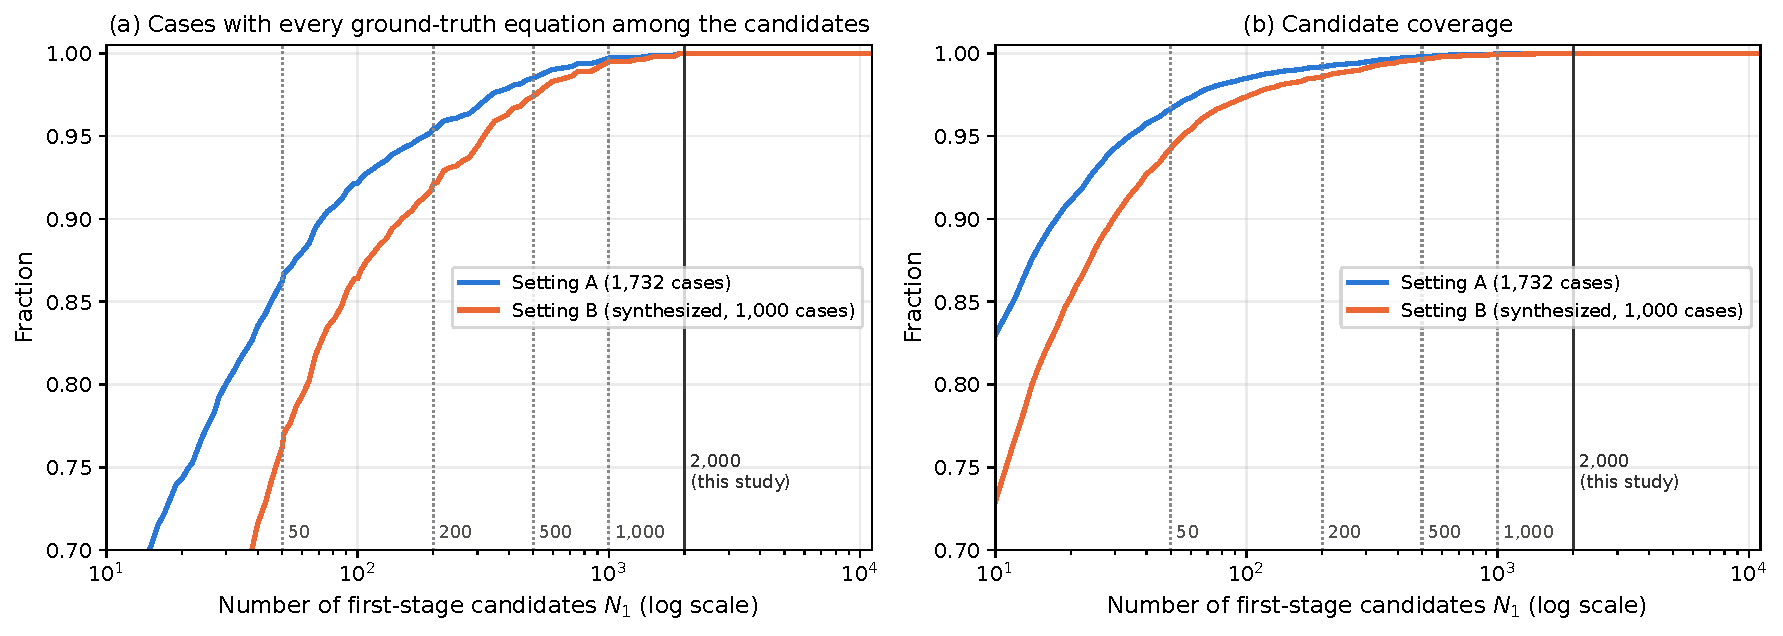
\includegraphics[width=\linewidth]{figures/fig_n1_coverage.pdf}
\caption{Number of first-stage candidates $N_1$ (log scale) and (a) the fraction of cases with
every ground-truth equation among the candidates and (b) the candidate coverage, the fraction of
ground-truth equations among the candidates (first-stage weights $(0.3, 0.7)$). Dotted lines mark
the values of $N_1$ compared in Table~\ref{tab:n1}, and the solid line the $N_1 = 2{,}000$ of this
thesis. Every ground-truth equation of every case enters the candidates at $N_1 = 1{,}880$.}
\label{fig:n1}
\end{figure}

\begin{table}[h]\centering
\caption{The proposed method (static reranking) with different numbers of first-stage candidates
$N_1$ (mean $\pm$ SD over 10 splits). Coverage is that of the test cases. Time is the wall-clock
time of one run of training and evaluation, with six runs in parallel.}
\label{tab:n1}
\footnotesize
\setlength{\tabcolsep}{3pt}
\begin{tabular}{@{}lrccccr@{}}
\toprule
 & $N_1$ & Coverage & Recall@20 & MAP & R-Precision & Time (s) \\
\midrule
Setting A & 50 & 0.9645 & $0.959 \pm 0.013$ & $0.845 \pm 0.052$ & $0.775 \pm 0.065$ & 54 \\
 & 200 & 0.9918 & $0.978 \pm 0.011$ & $0.857 \pm 0.055$ & $0.780 \pm 0.073$ & 60 \\
 & 500 & 0.9982 & $0.980 \pm 0.010$ & $0.859 \pm 0.054$ & $0.780 \pm 0.069$ & 70 \\
 & 1,000 & 0.9998 & $0.981 \pm 0.010$ & $0.858 \pm 0.055$ & $0.776 \pm 0.072$ & 125 \\
 & 2,000 & 1.0000 & $0.981 \pm 0.010$ & $0.860 \pm 0.053$ & $0.779 \pm 0.073$ & 162 \\
\midrule
Setting B & 50 & 0.9335 & $0.924 \pm 0.020$ & $0.798 \pm 0.041$ & $0.745 \pm 0.042$ & 35 \\
 & 200 & 0.9834 & $0.959 \pm 0.015$ & $0.824 \pm 0.041$ & $0.754 \pm 0.042$ & 38 \\
 & 500 & 0.9960 & $0.965 \pm 0.015$ & $0.829 \pm 0.043$ & $0.755 \pm 0.044$ & 43 \\
 & 1,000 & 0.9994 & $0.967 \pm 0.015$ & $0.832 \pm 0.041$ & $0.756 \pm 0.042$ & 71 \\
 & 2,000 & 1.0000 & $0.966 \pm 0.016$ & $0.832 \pm 0.041$ & $0.755 \pm 0.042$ & 87 \\
\bottomrule
\end{tabular}
\end{table}

\clearpage
\section{Literature Collection}
\label{app:papers}
Table~\ref{tab:search} gives the search term of each field and the numbers of PDFs obtained, and
Table~\ref{tab:papers} lists the 329 documents among the sources of the database (types follow the
OpenAlex classification as of 20 October 2026).

% 2026-10-21 generated by make_appendix_tables.py from docs/appendix_materials/search_terms.csv (English labels).
\begin{footnotesize}
\setlength{\tabcolsep}{3pt}
\begin{longtable}{@{}>{\raggedright\arraybackslash}p{0.17\linewidth}>{\raggedright\arraybackslash}p{0.40\linewidth}rrrrrrr@{}}
\caption{Search term of each field and the numbers of PDFs obtained. We sent each search term to OpenAlex followed by ``mathematical model differential equation.'' O counts the PDFs obtained by this search; F1--F3 count those obtained by the supplementary searches, which used three to five other search terms per field; P counts those obtained by the additional search for optics. The supplementary searches stopped when the field held 10 PDFs. ``DB'' counts the PDFs whose equations entered the database.}\label{tab:search}\\
\toprule
Field & Search term & O & F1 & F2 & F3 & P & Total & DB \\
\midrule
\endfirsthead
\toprule
Field & Search term & O & F1 & F2 & F3 & P & Total & DB \\
\midrule
\endhead
\bottomrule
\endlastfoot
Chem.\ eng.\ fundamentals & chemical process simulation steady state material balance & 4 & --- & 6 & --- & --- & 10 & 10 \\
Reaction eng.\ (basic) & CSTR PFR batch reactor design equation kinetics & 3 & 6 & --- & --- & --- & 9 & 9 \\
Reaction eng.\ (applied) & non-isothermal reactor catalytic reactor multiphase model & 6 & --- & --- & 4 & --- & 10 & 9 \\
Process control (basic) & process control PID transfer function dynamic & 6 & --- & --- & 4 & --- & 10 & 9 \\
Process control (applied) & model predictive control adaptive nonlinear process & 6 & --- & --- & 4 & --- & 10 & 10 \\
Thermodynamics (basic) & chemical thermodynamics phase equilibrium equation of state & 4 & --- & 3 & 3 & --- & 10 & 10 \\
Thermodynamics (applied) & polymer solution thermodynamics activity coefficient model & 1 & 4 & --- & 5 & --- & 10 & 10 \\
Fluid mechanics (basic) & fluid dynamics Navier Stokes viscous flow boundary & 9 & --- & --- & --- & --- & 9 & 9 \\
Fluid mechanics (applied) & turbulent flow multiphase CFD RANS LES simulation & 5 & --- & --- & 5 & --- & 10 & 10 \\
Heat transfer (basic) & heat transfer Fourier conduction convection radiation & 3 & 5 & --- & --- & --- & 8 & 7 \\
Heat transfer (applied) & shell tube heat exchanger numerical thermal design & 4 & --- & 4 & --- & --- & 8 & 8 \\
Mass transfer & mass transfer Fick diffusion coefficient concentration & 4 & --- & 5 & --- & --- & 9 & 9 \\
Transport phenomena & transport phenomena momentum heat mass coupled & 1 & 9 & --- & --- & --- & 10 & 10 \\
Separation processes & distillation column tray model MESH equations & 3 & 6 & --- & --- & --- & 9 & 9 \\
Electrochemistry (basic) & electrochemistry Butler Volmer Nernst Tafel electrode & 1 & 7 & --- & --- & --- & 8 & 8 \\
Electrochemistry (applied) & battery fuel cell electrolyzer mathematical model & 6 & --- & --- & 4 & --- & 10 & 10 \\
Bioprocesses & bioprocess fermentation Monod chemostat kinetic model & 6 & --- & --- & 4 & --- & 10 & 7 \\
Pharmaceutics & pharmaceutical dissolution pharmacokinetics compartment model & 2 & 8 & --- & --- & --- & 10 & 9 \\
Food engineering & food engineering drying thermal processing freezing & 1 & 8 & --- & --- & --- & 9 & 9 \\
Polymer engineering & polymerization reactor model molecular weight distribution kinetics & 6 & --- & --- & 4 & --- & 10 & 10 \\
Semiconductor physics & semiconductor device drift diffusion Shockley MOSFET & 3 & 7 & --- & --- & --- & 10 & 10 \\
Combustion & combustion flame propagation kinetic mechanism premixed & 4 & --- & 6 & --- & --- & 10 & 7 \\
Nuclear engineering & nuclear reactor neutron diffusion point kinetics & 3 & 6 & --- & --- & --- & 9 & 8 \\
HVAC & HVAC psychrometrics cooling load humidity ratio & 0 & 10 & --- & --- & --- & 10 & 8 \\
Environmental eng. & environmental pollutant transport advection diffusion treatment & 4 & --- & 6 & --- & --- & 10 & 10 \\
Optics & optics lens equation diffraction wave Maxwell & 5 & --- & --- & 2 & 3 & 10 & 10 \\
Acoustics & acoustics wave equation resonance impedance Helmholtz & 5 & --- & --- & 5 & --- & 10 & 10 \\
Aerodynamics & aerodynamics lift drag boundary layer airfoil & 3 & 3 & --- & 4 & --- & 10 & 10 \\
Mechanical vibration & mechanical vibration degree of freedom modal analysis & 2 & 8 & --- & --- & --- & 10 & 10 \\
Structural mechanics & structural mechanics beam bending stress strain & 3 & 5 & --- & --- & --- & 8 & 8 \\
Electrical engineering & RLC electrical circuit dynamic analysis state space & 7 & --- & --- & 3 & --- & 10 & 8 \\
Geotechnical eng. & geotechnical consolidation slope stability earth pressure & 4 & --- & 6 & --- & --- & 10 & 9 \\
\midrule
Total & & 124 & 92 & 36 & 51 & 3 & 306 & 290 \\
\end{longtable}
\end{footnotesize}

% 2026-10-21 generated by make_appendix_tables.py from docs/appendix_materials/papers_longtable.tex (English labels).
% Types follow the OpenAlex classification as of 2026-10-20 (it may differ from the classification at collection time).
\begin{footnotesize}
\setlength{\tabcolsep}{2.5pt}
\begin{longtable}{@{}r>{\raggedright\arraybackslash}p{0.31\linewidth}c>{\raggedright\arraybackslash}p{0.09\linewidth}>{\raggedright\arraybackslash}p{0.135\linewidth}>{\raggedright\arraybackslash}p{0.155\linewidth}cr@{}}
\caption{The 329 documents among the sources of the equation database. Route: M = collected by hand early in this work (24), S = retrieved by the Semantic Scholar search early in this work (15), O = the OpenAlex search by field (118), F1--F3 = the supplementary OpenAlex searches 1--3 (88, 33, and 48), P = the additional search for optics (3). A dagger (\dag) marks a title inferred from the file name and the equations in the database, because the PDF is not at hand. ``Eqs.'' gives the number of equations in the database. A document entered as several sources occupies one row per source.}\label{tab:papers}\\
\toprule
No. & Title (below: source identifier in the database) & Year & Type & Field & DOI / OpenAlex ID & Route & Eqs. \\
\midrule
\endfirsthead
\toprule
No. & Title (below: source identifier in the database) & Year & Type & Field & DOI / OpenAlex ID & Route & Eqs. \\
\midrule
\endhead
\midrule
\multicolumn{8}{r}{(continued on the next page)}\\
\endfoot
\bottomrule
\endlastfoot
1 & Unknown (a model of heat transfer in a hybrid CSTR plant)\newline {\scriptsize\texttt{038.\allowbreak{}pdf}} &  & unknown & Early & --- & M & 13 \\
2 & On the dynamic behavior of continuous stirred tank reactors\newline {\scriptsize\texttt{1-\allowbreak{}s2.\allowbreak{}0-\allowbreak{}0009250974800898-\allowbreak{}main.\allowbreak{}pdf}} & 1974 & article & Early & {\scriptsize\texttt{10.\allowbreak{}1016/\allowbreak{}0009-\allowbreak{}2509(74)\allowbreak{}80089-\allowbreak{}8}} & M & 33 \\
3 & Dynamic modeling of biodiesel production from simulated waste cooking oil using immobilized lipase\newline {\scriptsize\texttt{1-\allowbreak{}s2.\allowbreak{}0-\allowbreak{}S1369703X09000059-\allowbreak{}main.\allowbreak{}pdf}} & 2009 & article & Early & {\scriptsize\texttt{10.\allowbreak{}1016/\allowbreak{}j.\allowbreak{}bej.\allowbreak{}2009.\allowbreak{}01.\allowbreak{}003}} & M & 9 \\
4 & J.-P. Corriou, Process Control: Theory and Applications, 2nd ed.\ (Springer)\textsuperscript{\dag}\newline {\scriptsize\texttt{2018\_\allowbreak{}Book\_\allowbreak{}ProcessControl.\allowbreak{}pdf}} & 2018 & book & Early & {\scriptsize\texttt{10.\allowbreak{}1007/\allowbreak{}978-\allowbreak{}3-\allowbreak{}319-\allowbreak{}61143-\allowbreak{}3}} & M & 226 \\
5 & (apparently an excerpt of Chapter 1 of 2018\_Book\_ProcessControl.pdf)\textsuperscript{\dag}\newline {\scriptsize\texttt{2018\_\allowbreak{}Book\_\allowbreak{}ProcessControl\_\allowbreak{}Chapter1.\allowbreak{}pdf}} &  & unknown & Early & --- & M & 50 \\
6 & (apparently a part of Chapter 1 of 2018\_Book\_ProcessControl.pdf)\textsuperscript{\dag}\newline {\scriptsize\texttt{2018\_\allowbreak{}Book\_\allowbreak{}ProcessControl\_\allowbreak{}Chapter1\_\allowbreak{}6.\allowbreak{}pdf}} &  & unknown & Early & --- & M & 54 \\
7 & J.-P. Corriou, Process Control: Theory and Applications (Springer), Chapter 1\textsuperscript{\dag}\newline {\scriptsize\texttt{9781852337766-\allowbreak{}c1.\allowbreak{}pdf}} & 2004 & book chapter & Early & --- & M & 70 \\
8 & (apparently F. Haugen, Basic Dynamics and Control)\textsuperscript{\dag}\newline {\scriptsize\texttt{Basic\_\allowbreak{}Dyn\_\allowbreak{}Con\_\allowbreak{}Textbook\_\allowbreak{}free.\allowbreak{}pdf}} &  & book & Early & --- & M & 61 \\
9 & Unknown\newline {\scriptsize\texttt{Chemical Process Dynamics.\allowbreak{}pdf}} &  & unknown & Early & --- & M & 23 \\
10 & Chemical Process Dynamics and Controls (University of Michigan, open textbook, CC BY 3.0)\newline {\scriptsize\texttt{ChemicalProcessDynamicsAndControls.\allowbreak{}pdf}} &  & book & Early & --- & M & 521 \\
11 & (apparently Marlin, Process Control, Chapter 3, ``Mathematical Modelling Principles'')\textsuperscript{\dag}\newline {\scriptsize\texttt{Process\_\allowbreak{}Control\_\allowbreak{}Chapter3.\allowbreak{}pdf}} &  & book chapter & Early & --- & M & 79 \\
12 & (apparently Marlin, Process Control, Chapter 4, ``Modelling and Analysis for Process Control'')\textsuperscript{\dag}\newline {\scriptsize\texttt{Process\_\allowbreak{}Control\_\allowbreak{}Chapter4.\allowbreak{}pdf}} &  & book chapter & Early & --- & M & 82 \\
13 & T. E. Marlin, Process Control: Designing Processes and Control Systems for Dynamic Performance, 2nd ed.\ (McGraw-Hill; the version the author released free of charge in 2015)\newline {\scriptsize\texttt{Process\_\allowbreak{}Control\_\allowbreak{}Designing\_\allowbreak{}Processes\_\allowbreak{}and\_\allowbreak{}Control\_\allowbreak{}Systems\_\allowbreak{}for\_\allowbreak{}Dynamic\_\allowbreak{}Performance.\allowbreak{}pdf}} & 2000/2015 & book & Early & --- & M & 482 \\
14 & (apparently the list of symbols of a process-control textbook)\newline {\scriptsize\texttt{Process\_\allowbreak{}Control\_\allowbreak{}Symbols\_\allowbreak{}and\_\allowbreak{}Acronyms.\allowbreak{}pdf}} &  & unknown & Early & --- & M & 2 \\
15 & D. E. Seborg, T. F. Edgar, D. A. Mellichamp, F. J. Doyle III, Process Dynamics and Control, 3rd ed.\ (Wiley)\newline {\scriptsize\texttt{SEBORG\_\allowbreak{}3rd\_\allowbreak{}Edition\_\allowbreak{}Process\_\allowbreak{}Dynamics\_\allowbreak{}and.\allowbreak{}pdf}} & 2010 & book & Early & --- & M & 308 \\
16 & (apparently Seborg et al., Process Dynamics and Control, Chapter 2; edition unknown)\textsuperscript{\dag}\newline {\scriptsize\texttt{SEBORG\_\allowbreak{}Process\_\allowbreak{}Dynamic\_\allowbreak{}and\_\allowbreak{}Control\_\allowbreak{}Chap\_\allowbreak{}2.\allowbreak{}pdf}} &  & book chapter & Early & --- & M & 108 \\
17 & Unknown (a paper in World Journal of Engineering and Technology, 2015, on residence-time distributions)\newline {\scriptsize\texttt{WJET\_\allowbreak{}2015040715405408.\allowbreak{}pdf}} & 2015 & article & Early & --- & M & 6 \\
18 & Effects on Biodiesel Production Caused by Feed Oil Changes in a Continuous Stirred-Tank Reactor\newline {\scriptsize\texttt{applsci-\allowbreak{}10-\allowbreak{}00992-\allowbreak{}v2.\allowbreak{}pdf}} & 2020 & article & Early & {\scriptsize\texttt{10.\allowbreak{}3390/\allowbreak{}app10030992}} & M & 42 \\
19 & Synthesis of Guanidine and Its Deposition on Bacterial Cellulose as Green Heterogeneous Catalyst for Transesterification to Methyl Esters\newline {\scriptsize\texttt{energies-\allowbreak{}17-\allowbreak{}01344.\allowbreak{}pdf}} & 2024 & article & Early & {\scriptsize\texttt{10.\allowbreak{}3390/\allowbreak{}en17061344}} & M & 23 \\
20 & Kinetics of transesterification of soybean oil (Noureddini and Zhu, JAOCS)\textsuperscript{\dag}\newline {\scriptsize\texttt{kinetics\_\allowbreak{}soybean\_\allowbreak{}oil.\allowbreak{}pdf}} & 1997 & article & Early & {\scriptsize\texttt{10.\allowbreak{}1007/\allowbreak{}s11746-\allowbreak{}997-\allowbreak{}0254-\allowbreak{}2}} & M & 4 \\
21 & Mathematical modeling of transesterification process kinetics of triglycerides catalyzed by TMAH\newline {\scriptsize\texttt{matecconf\_\allowbreak{}cscc2019\_\allowbreak{}01027.\allowbreak{}pdf}} & 2019 & conference paper & Early & {\scriptsize\texttt{10.\allowbreak{}1051/\allowbreak{}matecconf/\allowbreak{}201929201027}} & M & 9 \\
22 & Need for Control: Instability of Continuous Stirred Tank Polymerization Reactor Simulations\newline {\scriptsize\texttt{need-\allowbreak{}for-\allowbreak{}control-\allowbreak{}instability-\allowbreak{}of-\allowbreak{}continuous-\allowbreak{}stirred-\allowbreak{}tank-\allowbreak{}polymerization-\allowbreak{}reactor-\allowbreak{}simulations.\allowbreak{}pdf}} & 2025 & article & Early & {\scriptsize\texttt{10.\allowbreak{}1021/\allowbreak{}acs.\allowbreak{}iecr.\allowbreak{}5c03903}} & M & 7 \\
23 & Modeling and simulation of biodiesel synthesis in fixed bed and packed bed membrane reactors using heterogeneous catalyst: a comparative study\newline {\scriptsize\texttt{s41598-\allowbreak{}024-\allowbreak{}60757-\allowbreak{}5.\allowbreak{}pdf}} & 2024 & article & Early & {\scriptsize\texttt{10.\allowbreak{}1038/\allowbreak{}s41598-\allowbreak{}024-\allowbreak{}60757-\allowbreak{}5}} & M & 46 \\
24 & Fuzzy logic Control of Continuous Stirred Tank Reactor\textsuperscript{\dag}\newline {\scriptsize\texttt{vol20no2p7.\allowbreak{}pdf}} & 2013 & article & Early & {\scriptsize\texttt{10.\allowbreak{}25130/\allowbreak{}tjes.\allowbreak{}20.\allowbreak{}2.\allowbreak{}07}} & M & 8 \\
25 & Modeling of an industrial process of pleuromutilin fermentation using feed-forward neural networks\newline {\scriptsize\texttt{2013\_\allowbreak{}Modeling\_\allowbreak{}of\_\allowbreak{}an\_\allowbreak{}industrial\_\allowbreak{}process\_\allowbreak{}of\_\allowbreak{}pleuromutilin\_\allowbreak{}fermentat.\allowbreak{}pdf}} & 2013 & article & Early & {\scriptsize\texttt{10.\allowbreak{}1590/\allowbreak{}s0104-\allowbreak{}66322013000100012}} & S & 15 \\
26 & Kinetic Modeling and Optimization of a Batch Ethanol Fermentation Process\newline {\scriptsize\texttt{2016\_\allowbreak{}Kinetic\_\allowbreak{}Modeling\_\allowbreak{}and\_\allowbreak{}Optimization\_\allowbreak{}of\_\allowbreak{}a\_\allowbreak{}Batch\_\allowbreak{}Ethanol\_\allowbreak{}Ferment.\allowbreak{}pdf}} & 2016 & article & Early & {\scriptsize\texttt{10.\allowbreak{}4172/\allowbreak{}2155-\allowbreak{}9821.\allowbreak{}1000266}} & S & 15 \\
27 & Current State and Perspective in the Models Applicable to Oenology\newline {\scriptsize\texttt{2018\_\allowbreak{}Current\_\allowbreak{}State\_\allowbreak{}and\_\allowbreak{}Perspective\_\allowbreak{}in\_\allowbreak{}the\_\allowbreak{}Models\_\allowbreak{}Applicable\_\allowbreak{}to\_\allowbreak{}Oe.\allowbreak{}pdf}} & 2018 & book chapter & Early & {\scriptsize\texttt{10.\allowbreak{}5772/\allowbreak{}intechopen.\allowbreak{}71711}} & S & 61 \\
28 & An experimental and modeling study of ammonia with enriched oxygen content and ammonia/hydrogen laminar flame speed at elevated pressure and temperature\newline {\scriptsize\texttt{2021\_\allowbreak{}An\_\allowbreak{}experimental\_\allowbreak{}and\_\allowbreak{}modeling\_\allowbreak{}study\_\allowbreak{}of\_\allowbreak{}ammonia\_\allowbreak{}with\_\allowbreak{}enriched.\allowbreak{}pdf}} & 2021 & article & Early & {\scriptsize\texttt{10.\allowbreak{}1016/\allowbreak{}j.\allowbreak{}proci.\allowbreak{}2020.\allowbreak{}06.\allowbreak{}197}} & S & 3 \\
29 & Evolution of Flame Displacement Speed Within Flame Front in Different Regimes of Premixed Turbulent Combustion\newline {\scriptsize\texttt{2023\_\allowbreak{}Evolution\_\allowbreak{}of\_\allowbreak{}Flame\_\allowbreak{}Displacement\_\allowbreak{}Speed\_\allowbreak{}Within\_\allowbreak{}Flame\_\allowbreak{}Front\_\allowbreak{}in.\allowbreak{}pdf}} & 2023 & article & Early & {\scriptsize\texttt{10.\allowbreak{}1007/\allowbreak{}s10494-\allowbreak{}023-\allowbreak{}00494-\allowbreak{}3}} & S & 11 \\
30 & On flame speed enhancement in turbulent premixed hydrogen-air flames during local flame-flame interaction\newline {\scriptsize\texttt{2023\_\allowbreak{}On\_\allowbreak{}flame\_\allowbreak{}speed\_\allowbreak{}enhancement\_\allowbreak{}in\_\allowbreak{}turbulent\_\allowbreak{}premixed\_\allowbreak{}hydrogen-\allowbreak{}ai.\allowbreak{}pdf}} & 2023 & article & Early & {\scriptsize\texttt{10.\allowbreak{}1016/\allowbreak{}j.\allowbreak{}combustflame.\allowbreak{}2023.\allowbreak{}113017}} & S & 27 \\
31 & Experimentally Closing the Balance of Progress of Reaction in Premixed Turbulent Combustion in the Thin Flame Regime\newline {\scriptsize\texttt{2024\_\allowbreak{}Experimentally\_\allowbreak{}Closing\_\allowbreak{}the\_\allowbreak{}Balance\_\allowbreak{}of\_\allowbreak{}Progress\_\allowbreak{}of\_\allowbreak{}Reaction\_\allowbreak{}i.\allowbreak{}pdf}} & 2024 & article & Early & {\scriptsize\texttt{10.\allowbreak{}1007/\allowbreak{}s10494-\allowbreak{}024-\allowbreak{}00538-\allowbreak{}2}} & S & 41 \\
32 & A new simple dynamic model of parallel and counter flow heat exchangers based on their static and structural characteristics.\newline {\scriptsize\texttt{1989\_\allowbreak{}A\_\allowbreak{}new\_\allowbreak{}simple\_\allowbreak{}dynamic\_\allowbreak{}model\_\allowbreak{}of\_\allowbreak{}parallel\_\allowbreak{}and\_\allowbreak{}counter\_\allowbreak{}flow\_\allowbreak{}heat.\allowbreak{}pdf}} & 1989 & article & Early & {\scriptsize\texttt{10.\allowbreak{}1299/\allowbreak{}kikaic.\allowbreak{}55.\allowbreak{}119}} & S & 13 \\
33 & A Dynamic Model for Helium Core Heat Exchangers\newline {\scriptsize\texttt{1990\_\allowbreak{}A\_\allowbreak{}dynamic\_\allowbreak{}model\_\allowbreak{}for\_\allowbreak{}helium\_\allowbreak{}core\_\allowbreak{}heat\_\allowbreak{}exchangers.\allowbreak{}pdf}} & 1990 & book chapter & Early & {\scriptsize\texttt{10.\allowbreak{}1007/\allowbreak{}978-\allowbreak{}1-\allowbreak{}4615-\allowbreak{}3728-\allowbreak{}1\_20}} & S & 40 \\
34 & Towards the modelling of a heat‐exchanger reactor by a dynamic approach\newline {\scriptsize\texttt{2015\_\allowbreak{}Towards\_\allowbreak{}the\_\allowbreak{}modelling\_\allowbreak{}of\_\allowbreak{}a\_\allowbreak{}heat\_\allowbreak{}exchanger\_\allowbreak{}reactor\_\allowbreak{}by\_\allowbreak{}a\_\allowbreak{}dynam.\allowbreak{}pdf}} & 2015 & article & Early & {\scriptsize\texttt{10.\allowbreak{}1002/\allowbreak{}cjce.\allowbreak{}22119}} & S & 18 \\
35 & Numerical Solutions of Free Convective Flow from a Vertical Cone with Mass Transfer under the Influence of Chemical Reaction and Heat Generation/Absorption in the Presence of UWT/UWC\newline {\scriptsize\texttt{2016\_\allowbreak{}Numerical\_\allowbreak{}Solutions\_\allowbreak{}of\_\allowbreak{}Free\_\allowbreak{}Convective\_\allowbreak{}Flow\_\allowbreak{}from\_\allowbreak{}a\_\allowbreak{}Vertical.\allowbreak{}pdf}} & 2016 & article & Early & {\scriptsize\texttt{10.\allowbreak{}18869/\allowbreak{}acadpub.\allowbreak{}jafm.\allowbreak{}68.\allowbreak{}224.\allowbreak{}24062}} & S & 19 \\
36 & A study of triple-mass diffusion species and energy transfer in Carreau–Yasuda material influenced by activation energy and heat source\newline {\scriptsize\texttt{2022\_\allowbreak{}A\_\allowbreak{}study\_\allowbreak{}of\_\allowbreak{}triple-\allowbreak{}mass\_\allowbreak{}diffusion\_\allowbreak{}species\_\allowbreak{}and\_\allowbreak{}energy\_\allowbreak{}transfer.\allowbreak{}pdf}} & 2022 & article & Early & {\scriptsize\texttt{10.\allowbreak{}1038/\allowbreak{}s41598-\allowbreak{}022-\allowbreak{}13890-\allowbreak{}y}} & S & 23 \\
37 & General route to design polymer molecular weight distributions through flow chemistry\newline {\scriptsize\texttt{2020\_\allowbreak{}General\_\allowbreak{}route\_\allowbreak{}to\_\allowbreak{}design\_\allowbreak{}polymer\_\allowbreak{}molecular\_\allowbreak{}weight\_\allowbreak{}distributio.\allowbreak{}pdf}} & 2020 & article & Early & {\scriptsize\texttt{10.\allowbreak{}1038/\allowbreak{}s41467-\allowbreak{}020-\allowbreak{}16874-\allowbreak{}6}} & S & 2 \\
38 & Chemical reactor stability research of ethylene polymerization\newline {\scriptsize\texttt{2023\_\allowbreak{}Chemical\_\allowbreak{}reactor\_\allowbreak{}stability\_\allowbreak{}research\_\allowbreak{}of\_\allowbreak{}ethylene\_\allowbreak{}polymerizati.\allowbreak{}pdf}} & 2023 & article & Early & {\scriptsize\texttt{10.\allowbreak{}24143/\allowbreak{}2072-\allowbreak{}9502-\allowbreak{}2023-\allowbreak{}4-\allowbreak{}17-\allowbreak{}25}} & S & 11 \\
39 & Mathematical modeling of pyrolysis of rubber waste in horizontal cylindrical reactor\newline {\scriptsize\texttt{2024\_\allowbreak{}Mathematical\_\allowbreak{}modeling\_\allowbreak{}of\_\allowbreak{}pyrolysis\_\allowbreak{}of\_\allowbreak{}rubber\_\allowbreak{}waste\_\allowbreak{}in\_\allowbreak{}horizo.\allowbreak{}pdf}} & 2024 & article & Early & {\scriptsize\texttt{10.\allowbreak{}17588/\allowbreak{}2072-\allowbreak{}2672.\allowbreak{}2024.\allowbreak{}2.\allowbreak{}092-\allowbreak{}099}} & S & 9 \\
40 & Analytical solution for a hybrid Logistic‐Monod cell growth model in batch and continuous stirred tank reactor culture\newline {\scriptsize\texttt{02\_\allowbreak{}Analytical\_\allowbreak{}solution\_\allowbreak{}for\_\allowbreak{}a\_\allowbreak{}hybrid\_\allowbreak{}Logistic\_\allowbreak{}Monod\_\allowbreak{}cell\_\allowbreak{}growth\_\allowbreak{}\_\allowbreak{}2019.\allowbreak{}pdf}} & 2019 & article & Bioprocesses & {\scriptsize\texttt{10.\allowbreak{}1002/\allowbreak{}bit.\allowbreak{}27230}} & O & 18 \\
41 & A novel process-based model of microbial growth: self-inhibition in Saccharomyces cerevisiae aerobic fed-batch cultures\newline {\scriptsize\texttt{04\_\allowbreak{}A\_\allowbreak{}novel\_\allowbreak{}process-\allowbreak{}based\_\allowbreak{}model\_\allowbreak{}of\_\allowbreak{}microbial\_\allowbreak{}growth\_\allowbreak{}self-\allowbreak{}inhibit\_\allowbreak{}2015.\allowbreak{}pdf}} & 2015 & article & Bioprocesses & {\scriptsize\texttt{10.\allowbreak{}1186/\allowbreak{}s12934-\allowbreak{}015-\allowbreak{}0295-\allowbreak{}4}} & O & 20 \\
42 & Modeling growth, lipid accumulation and lipid turnover in submerged batch cultures of Umbelopsis isabellina\newline {\scriptsize\texttt{06\_\allowbreak{}Modeling\_\allowbreak{}growth\_\allowbreak{}lipid\_\allowbreak{}accumulation\_\allowbreak{}and\_\allowbreak{}lipid\_\allowbreak{}turnover\_\allowbreak{}in\_\allowbreak{}sub\_\allowbreak{}2011.\allowbreak{}pdf}} & 2011 & article & Bioprocesses & {\scriptsize\texttt{10.\allowbreak{}1007/\allowbreak{}s00449-\allowbreak{}011-\allowbreak{}0632-\allowbreak{}x}} & O & 19 \\
43 & Bridging substrate intake kinetics and bacterial growth phenotypes with flux balance analysis incorporating proteome allocation\newline {\scriptsize\texttt{09\_\allowbreak{}Bridging\_\allowbreak{}substrate\_\allowbreak{}intake\_\allowbreak{}kinetics\_\allowbreak{}and\_\allowbreak{}bacterial\_\allowbreak{}growth\_\allowbreak{}phen\_\allowbreak{}2020.\allowbreak{}pdf}} & 2020 & article & Bioprocesses & {\scriptsize\texttt{10.\allowbreak{}1038/\allowbreak{}s41598-\allowbreak{}020-\allowbreak{}61174-\allowbreak{}0}} & O & 20 \\
44 & The Future of Pharmaceutical Manufacturing Sciences\newline {\scriptsize\texttt{01\_\allowbreak{}The\_\allowbreak{}Future\_\allowbreak{}of\_\allowbreak{}Pharmaceutical\_\allowbreak{}Manufacturing\_\allowbreak{}Sciences\_\allowbreak{}2015.\allowbreak{}pdf}} & 2015 & article & Process control (basic) & {\scriptsize\texttt{10.\allowbreak{}1002/\allowbreak{}jps.\allowbreak{}24594}} & O & 2 \\
45 & A Review of Quadrotor Unmanned Aerial Vehicles: Applications, Architectural Design and Control Algorithms\newline {\scriptsize\texttt{02\_\allowbreak{}A\_\allowbreak{}Review\_\allowbreak{}of\_\allowbreak{}Quadrotor\_\allowbreak{}Unmanned\_\allowbreak{}Aerial\_\allowbreak{}Vehicles\_\allowbreak{}Applications\_\allowbreak{}\_\allowbreak{}2022.\allowbreak{}pdf}} & 2022 & article & Process control (basic) & {\scriptsize\texttt{10.\allowbreak{}1007/\allowbreak{}s10846-\allowbreak{}021-\allowbreak{}01527-\allowbreak{}7}} & O & 23 \\
46 & Optimal Tuning of Fractional Order PID Controller for DC Motor Speed Control via Chaotic Atom Search Optimization Algorithm\newline {\scriptsize\texttt{03\_\allowbreak{}Optimal\_\allowbreak{}Tuning\_\allowbreak{}of\_\allowbreak{}Fractional\_\allowbreak{}Order\_\allowbreak{}PID\_\allowbreak{}Controller\_\allowbreak{}for\_\allowbreak{}DC\_\allowbreak{}Mot\_\allowbreak{}2019.\allowbreak{}pdf}} & 2019 & article & Process control (basic) & {\scriptsize\texttt{10.\allowbreak{}1109/\allowbreak{}access.\allowbreak{}2019.\allowbreak{}2905961}} & O & 39 \\
47 & Bond-graph modeling\newline {\scriptsize\texttt{04\_\allowbreak{}Bond-\allowbreak{}graph\_\allowbreak{}modeling\_\allowbreak{}2007.\allowbreak{}pdf}} & 2007 & article & Process control (basic) & {\scriptsize\texttt{10.\allowbreak{}1109/\allowbreak{}mcs.\allowbreak{}2007.\allowbreak{}338279}} & O & 29 \\
48 & Towards Industrialization of FOPID Controllers: A Survey on Milestones of Fractional-Order Control and Pathways for Future Developments\newline {\scriptsize\texttt{05\_\allowbreak{}Towards\_\allowbreak{}Industrialization\_\allowbreak{}of\_\allowbreak{}FOPID\_\allowbreak{}Controllers\_\allowbreak{}A\_\allowbreak{}Survey\_\allowbreak{}on\_\allowbreak{}M\_\allowbreak{}2021.\allowbreak{}pdf}} & 2021 & article & Process control (basic) & {\scriptsize\texttt{10.\allowbreak{}1109/\allowbreak{}access.\allowbreak{}2021.\allowbreak{}3055117}} & O & 15 \\
49 & Moving beyond photosynthesis: from carbon source to sink‐driven vegetation modeling\newline {\scriptsize\texttt{01\_\allowbreak{}Moving\_\allowbreak{}beyond\_\allowbreak{}photosynthesis\_\allowbreak{}from\_\allowbreak{}carbon\_\allowbreak{}source\_\allowbreak{}to\_\allowbreak{}sink\_\allowbreak{}driv\_\allowbreak{}2013.\allowbreak{}pdf}} & 2013 & article & Process control (applied) & {\scriptsize\texttt{10.\allowbreak{}1111/\allowbreak{}nph.\allowbreak{}12614}} & O & 2 \\
50 & Stan : A Probabilistic Programming Language\newline {\scriptsize\texttt{02\_\allowbreak{}i\_\allowbreak{}Stan\_\allowbreak{}i\_\allowbreak{}A\_\allowbreak{}Probabilistic\_\allowbreak{}Programming\_\allowbreak{}Language\_\allowbreak{}2017.\allowbreak{}pdf}} & 2017 & article & Process control (applied) & {\scriptsize\texttt{10.\allowbreak{}18637/\allowbreak{}jss.\allowbreak{}v076.\allowbreak{}i01}} & O & 26 \\
51 & On Pixel-Wise Explanations for Non-Linear Classifier Decisions by Layer-Wise Relevance Propagation\newline {\scriptsize\texttt{03\_\allowbreak{}On\_\allowbreak{}Pixel-\allowbreak{}Wise\_\allowbreak{}Explanations\_\allowbreak{}for\_\allowbreak{}Non-\allowbreak{}Linear\_\allowbreak{}Classifier\_\allowbreak{}Decisio\_\allowbreak{}2015.\allowbreak{}pdf}} & 2015 & article & Process control (applied) & {\scriptsize\texttt{10.\allowbreak{}1371/\allowbreak{}journal.\allowbreak{}pone.\allowbreak{}0130140}} & O & 65 \\
52 & Machine Learning for Fluid Mechanics\newline {\scriptsize\texttt{04\_\allowbreak{}Machine\_\allowbreak{}Learning\_\allowbreak{}for\_\allowbreak{}Fluid\_\allowbreak{}Mechanics\_\allowbreak{}2019.\allowbreak{}pdf}} & 2019 & review & Process control (applied) & {\scriptsize\texttt{10.\allowbreak{}1146/\allowbreak{}annurev-\allowbreak{}fluid-\allowbreak{}010719-\allowbreak{}060214}} & O & 4 \\
53 & Digital Twin: Values, Challenges and Enablers From a Modeling Perspective\newline {\scriptsize\texttt{07\_\allowbreak{}Digital\_\allowbreak{}Twin\_\allowbreak{}Values\_\allowbreak{}Challenges\_\allowbreak{}and\_\allowbreak{}Enablers\_\allowbreak{}From\_\allowbreak{}a\_\allowbreak{}Modeling\_\allowbreak{}\_\allowbreak{}2020.\allowbreak{}pdf}} & 2020 & article & Process control (applied) & {\scriptsize\texttt{10.\allowbreak{}1109/\allowbreak{}access.\allowbreak{}2020.\allowbreak{}2970143}} & O & 1 \\
54 & Dynamical Movement Primitives: Learning Attractor Models for Motor Behaviors\newline {\scriptsize\texttt{08\_\allowbreak{}Dynamical\_\allowbreak{}Movement\_\allowbreak{}Primitives\_\allowbreak{}Learning\_\allowbreak{}Attractor\_\allowbreak{}Models\_\allowbreak{}for\_\allowbreak{}\_\allowbreak{}2012.\allowbreak{}pdf}} & 2012 & article & Process control (applied) & {\scriptsize\texttt{10.\allowbreak{}1162/\allowbreak{}neco\_a\_00393}} & O & 33 \\
55 & Two-phase flow of dusty fluid with suspended hybrid nanoparticles over a stretching cylinder with modified Fourier heat flux\newline {\scriptsize\texttt{06\_\allowbreak{}Two-\allowbreak{}phase\_\allowbreak{}flow\_\allowbreak{}of\_\allowbreak{}dusty\_\allowbreak{}fluid\_\allowbreak{}with\_\allowbreak{}suspended\_\allowbreak{}hybrid\_\allowbreak{}nanopart\_\allowbreak{}2021.\allowbreak{}pdf}} & 2021 & article & Heat transfer (basic) & {\scriptsize\texttt{10.\allowbreak{}1007/\allowbreak{}s42452-\allowbreak{}021-\allowbreak{}04364-\allowbreak{}3}} & O & 15 \\
56 & Numerically analysis of Marangoni convective flow of hybrid nanofluid over an infinite disk with thermophoresis particle deposition\newline {\scriptsize\texttt{08\_\allowbreak{}Numerically\_\allowbreak{}analysis\_\allowbreak{}of\_\allowbreak{}Marangoni\_\allowbreak{}convective\_\allowbreak{}flow\_\allowbreak{}of\_\allowbreak{}hybrid\_\allowbreak{}\_\allowbreak{}2023.\allowbreak{}pdf}} & 2023 & article & Heat transfer (basic) & {\scriptsize\texttt{10.\allowbreak{}1038/\allowbreak{}s41598-\allowbreak{}023-\allowbreak{}32011-\allowbreak{}x}} & O & 44 \\
57 & The Review of Some Commonly Used Methods and Techniques to Measure the Thermal Conductivity of Insulation Materials\newline {\scriptsize\texttt{09\_\allowbreak{}The\_\allowbreak{}Review\_\allowbreak{}of\_\allowbreak{}Some\_\allowbreak{}Commonly\_\allowbreak{}Used\_\allowbreak{}Methods\_\allowbreak{}and\_\allowbreak{}Techniques\_\allowbreak{}to\_\allowbreak{}M\_\allowbreak{}2016.\allowbreak{}pdf}} & 2016 & book chapter & Heat transfer (basic) & {\scriptsize\texttt{10.\allowbreak{}5772/\allowbreak{}64157}} & O & 6 \\
58 & A review on nanofluids - part I: theoretical and numerical investigations\newline {\scriptsize\texttt{01\_\allowbreak{}A\_\allowbreak{}review\_\allowbreak{}on\_\allowbreak{}nanofluids\_\allowbreak{}-\allowbreak{}\_\allowbreak{}part\_\allowbreak{}I\_\allowbreak{}theoretical\_\allowbreak{}and\_\allowbreak{}numerical\_\allowbreak{}in\_\allowbreak{}2008.\allowbreak{}pdf}} & 2008 & article & Heat transfer (applied) & {\scriptsize\texttt{10.\allowbreak{}1590/\allowbreak{}s0104-\allowbreak{}66322008000400001}} & O & 22 \\
59 & Water Desalination Using a Humidification-Dehumidification Technique—A Detailed Review\newline {\scriptsize\texttt{04\_\allowbreak{}Water\_\allowbreak{}Desalination\_\allowbreak{}Using\_\allowbreak{}a\_\allowbreak{}Humidification-\allowbreak{}Dehumidification\_\allowbreak{}T\_\allowbreak{}2013.\allowbreak{}pdf}} & 2013 & article & Heat transfer (applied) & {\scriptsize\texttt{10.\allowbreak{}4236/\allowbreak{}nr.\allowbreak{}2013.\allowbreak{}43036}} & O & 3 \\
60 & Review of applications of TLBO algorithm and a tutorial for beginners to solve the unconstrained and constrained optimization problems\newline {\scriptsize\texttt{06\_\allowbreak{}Review\_\allowbreak{}of\_\allowbreak{}applications\_\allowbreak{}of\_\allowbreak{}TLBO\_\allowbreak{}algorithm\_\allowbreak{}and\_\allowbreak{}a\_\allowbreak{}tutorial\_\allowbreak{}for\_\allowbreak{}\_\allowbreak{}2015.\allowbreak{}pdf}} & 2015 & article & Heat transfer (applied) & {\scriptsize\texttt{10.\allowbreak{}5267/\allowbreak{}j.\allowbreak{}dsl.\allowbreak{}2015.\allowbreak{}9.\allowbreak{}003}} & O & 10 \\
61 & A novel hybridity model for TiO2-CuO/water hybrid nanofluid flow over a static/moving wedge or corner\newline {\scriptsize\texttt{08\_\allowbreak{}A\_\allowbreak{}novel\_\allowbreak{}hybridity\_\allowbreak{}model\_\allowbreak{}for\_\allowbreak{}TiO2-\allowbreak{}CuO\_\allowbreak{}water\_\allowbreak{}hybrid\_\allowbreak{}nanofluid\_\allowbreak{}\_\allowbreak{}2019.\allowbreak{}pdf}} & 2019 & article & Heat transfer (applied) & {\scriptsize\texttt{10.\allowbreak{}1038/\allowbreak{}s41598-\allowbreak{}019-\allowbreak{}52720-\allowbreak{}6}} & O & 19 \\
62 & Global optimization of metasurface designs using statistical learning methods\newline {\scriptsize\texttt{01\_\allowbreak{}Global\_\allowbreak{}optimization\_\allowbreak{}of\_\allowbreak{}metasurface\_\allowbreak{}designs\_\allowbreak{}using\_\allowbreak{}statistical\_\allowbreak{}2019.\allowbreak{}pdf}} & 2019 & article & Optics & {\scriptsize\texttt{10.\allowbreak{}1038/\allowbreak{}s41598-\allowbreak{}019-\allowbreak{}53878-\allowbreak{}9}} & O & 1 \\
63 & Optical tweezers: theory and practice\newline {\scriptsize\texttt{02\_\allowbreak{}Optical\_\allowbreak{}tweezers\_\allowbreak{}theory\_\allowbreak{}and\_\allowbreak{}practice\_\allowbreak{}2020.\allowbreak{}pdf}} & 2020 & article & Optics & {\scriptsize\texttt{10.\allowbreak{}1140/\allowbreak{}epjp/\allowbreak{}s13360-\allowbreak{}020-\allowbreak{}00843-\allowbreak{}5}} & O & 65 \\
64 & Active learning of deep surrogates for PDEs: application to metasurface design\newline {\scriptsize\texttt{05\_\allowbreak{}Active\_\allowbreak{}learning\_\allowbreak{}of\_\allowbreak{}deep\_\allowbreak{}surrogates\_\allowbreak{}for\_\allowbreak{}PDEs\_\allowbreak{}application\_\allowbreak{}to\_\allowbreak{}m\_\allowbreak{}2020.\allowbreak{}pdf}} & 2020 & article & Optics & {\scriptsize\texttt{10.\allowbreak{}1038/\allowbreak{}s41524-\allowbreak{}020-\allowbreak{}00431-\allowbreak{}2}} & O & 11 \\
65 & Roadmap on transformation optics\newline {\scriptsize\texttt{06\_\allowbreak{}Roadmap\_\allowbreak{}on\_\allowbreak{}transformation\_\allowbreak{}optics\_\allowbreak{}2018.\allowbreak{}pdf}} & 2018 & article & Optics & {\scriptsize\texttt{10.\allowbreak{}1088/\allowbreak{}2040-\allowbreak{}8986/\allowbreak{}aab976}} & O & 4 \\
66 & Gravitational spin Hall effect of light\newline {\scriptsize\texttt{08\_\allowbreak{}Gravitational\_\allowbreak{}spin\_\allowbreak{}Hall\_\allowbreak{}effect\_\allowbreak{}of\_\allowbreak{}light\_\allowbreak{}2020.\allowbreak{}pdf}} & 2020 & article & Optics & {\scriptsize\texttt{10.\allowbreak{}1103/\allowbreak{}physrevd.\allowbreak{}102.\allowbreak{}024075}} & O & 110 \\
67 & RETRACTED: Theoretical investigations on the effect of absorbent type on carbon dioxide capture in hollow-fiber membrane contactors\newline {\scriptsize\texttt{03\_\allowbreak{}Theoretical\_\allowbreak{}investigations\_\allowbreak{}on\_\allowbreak{}the\_\allowbreak{}effect\_\allowbreak{}of\_\allowbreak{}absorbent\_\allowbreak{}type\_\allowbreak{}o\_\allowbreak{}2020.\allowbreak{}pdf}} & 2020 & article & Separation processes & {\scriptsize\texttt{10.\allowbreak{}1371/\allowbreak{}journal.\allowbreak{}pone.\allowbreak{}0236367}} & O & 21 \\
68 & Conceptual methods for synthesis of reactive distillation processes: recent developments and perspectives\newline {\scriptsize\texttt{05\_\allowbreak{}Conceptual\_\allowbreak{}methods\_\allowbreak{}for\_\allowbreak{}synthesis\_\allowbreak{}of\_\allowbreak{}reactive\_\allowbreak{}distillation\_\allowbreak{}pr\_\allowbreak{}2024.\allowbreak{}pdf}} & 2024 & article & Separation processes & {\scriptsize\texttt{10.\allowbreak{}1002/\allowbreak{}jctb.\allowbreak{}7633}} & O & 13 \\
69 & Modelling of displacement washing of packed bed of fibers\newline {\scriptsize\texttt{09\_\allowbreak{}Modelling\_\allowbreak{}of\_\allowbreak{}displacement\_\allowbreak{}washing\_\allowbreak{}of\_\allowbreak{}packed\_\allowbreak{}bed\_\allowbreak{}of\_\allowbreak{}fibers\_\allowbreak{}2009.\allowbreak{}pdf}} & 2009 & article & Separation processes & {\scriptsize\texttt{10.\allowbreak{}1590/\allowbreak{}s0104-\allowbreak{}66322009000200016}} & O & 21 \\
70 & Theory of Star Formation\newline {\scriptsize\texttt{01\_\allowbreak{}Theory\_\allowbreak{}of\_\allowbreak{}Star\_\allowbreak{}Formation\_\allowbreak{}2007.\allowbreak{}pdf}} & 2007 & review & Chem.\ eng.\ fundamentals & {\scriptsize\texttt{10.\allowbreak{}1146/\allowbreak{}annurev.\allowbreak{}astro.\allowbreak{}45.\allowbreak{}051806.\allowbreak{}110602}} & O & 56 \\
71 & Review: liquid phase sintering\newline {\scriptsize\texttt{02\_\allowbreak{}Review\_\allowbreak{}liquid\_\allowbreak{}phase\_\allowbreak{}sintering\_\allowbreak{}2008.\allowbreak{}pdf}} & 2008 & article & Chem.\ eng.\ fundamentals & {\scriptsize\texttt{10.\allowbreak{}1007/\allowbreak{}s10853-\allowbreak{}008-\allowbreak{}3008-\allowbreak{}0}} & O & 50 \\
72 & Dynamic rerouting of the carbohydrate flux is key to counteracting oxidative stress\newline {\scriptsize\texttt{05\_\allowbreak{}Dynamic\_\allowbreak{}rerouting\_\allowbreak{}of\_\allowbreak{}the\_\allowbreak{}carbohydrate\_\allowbreak{}flux\_\allowbreak{}is\_\allowbreak{}key\_\allowbreak{}to\_\allowbreak{}counter\_\allowbreak{}2007.\allowbreak{}pdf}} & 2007 & article & Chem.\ eng.\ fundamentals & {\scriptsize\texttt{10.\allowbreak{}1186/\allowbreak{}jbiol61}} & O & 5 \\
73 & Causes of variation in soil carbon simulations from CMIP5 Earth system models and comparison with observations\newline {\scriptsize\texttt{06\_\allowbreak{}Causes\_\allowbreak{}of\_\allowbreak{}variation\_\allowbreak{}in\_\allowbreak{}soil\_\allowbreak{}carbon\_\allowbreak{}simulations\_\allowbreak{}from\_\allowbreak{}CMIP5\_\allowbreak{}Ea\_\allowbreak{}2013.\allowbreak{}pdf}} & 2013 & article & Chem.\ eng.\ fundamentals & {\scriptsize\texttt{10.\allowbreak{}5194/\allowbreak{}bg-\allowbreak{}10-\allowbreak{}1717-\allowbreak{}2013}} & O & 8 \\
74 & Steady-State Simulation of Semiconductor Devices Using Discontinuous Galerkin Methods\newline {\scriptsize\texttt{03\_\allowbreak{}Steady-\allowbreak{}State\_\allowbreak{}Simulation\_\allowbreak{}of\_\allowbreak{}Semiconductor\_\allowbreak{}Devices\_\allowbreak{}Using\_\allowbreak{}Disco\_\allowbreak{}2020.\allowbreak{}pdf}} & 2020 & article & Semiconductor physics & {\scriptsize\texttt{10.\allowbreak{}1109/\allowbreak{}access.\allowbreak{}2020.\allowbreak{}2967125}} & O & 36 \\
75 & 3D finite element modeling and simulation of industrial semiconductor devices including impact ionization\newline {\scriptsize\texttt{04\_\allowbreak{}3D\_\allowbreak{}finite\_\allowbreak{}element\_\allowbreak{}modeling\_\allowbreak{}and\_\allowbreak{}simulation\_\allowbreak{}of\_\allowbreak{}industrial\_\allowbreak{}semi\_\allowbreak{}2015.\allowbreak{}pdf}} & 2015 & article & Semiconductor physics & {\scriptsize\texttt{10.\allowbreak{}1186/\allowbreak{}s13362-\allowbreak{}015-\allowbreak{}0015-\allowbreak{}z}} & O & 40 \\
76 & A review of recent advances in the spherical harmonics expansion method for semiconductor device simulation\newline {\scriptsize\texttt{05\_\allowbreak{}A\_\allowbreak{}review\_\allowbreak{}of\_\allowbreak{}recent\_\allowbreak{}advances\_\allowbreak{}in\_\allowbreak{}the\_\allowbreak{}spherical\_\allowbreak{}harmonics\_\allowbreak{}expan\_\allowbreak{}2016.\allowbreak{}pdf}} & 2016 & article & Semiconductor physics & {\scriptsize\texttt{10.\allowbreak{}1007/\allowbreak{}s10825-\allowbreak{}016-\allowbreak{}0828-\allowbreak{}z}} & O & 39 \\
77 & BISON: A Flexible Code for Advanced Simulation of the Performance of Multiple Nuclear Fuel Forms\newline {\scriptsize\texttt{03\_\allowbreak{}BISON\_\allowbreak{}A\_\allowbreak{}Flexible\_\allowbreak{}Code\_\allowbreak{}for\_\allowbreak{}Advanced\_\allowbreak{}Simulation\_\allowbreak{}of\_\allowbreak{}the\_\allowbreak{}Perform\_\allowbreak{}2021.\allowbreak{}pdf}} & 2021 & article & Nuclear engineering & {\scriptsize\texttt{10.\allowbreak{}1080/\allowbreak{}00295450.\allowbreak{}2020.\allowbreak{}1836940}} & O & 2 \\
78 & Small Modular Reactors: An Overview of Modeling, Control, Simulation, and Applications\newline {\scriptsize\texttt{08\_\allowbreak{}Small\_\allowbreak{}Modular\_\allowbreak{}Reactors\_\allowbreak{}An\_\allowbreak{}Overview\_\allowbreak{}of\_\allowbreak{}Modeling\_\allowbreak{}Control\_\allowbreak{}Simul\_\allowbreak{}2024.\allowbreak{}pdf}} & 2024 & article & Nuclear engineering & {\scriptsize\texttt{10.\allowbreak{}1109/\allowbreak{}access.\allowbreak{}2024.\allowbreak{}3351220}} & O & 1 \\
79 & Extracting Knowledge from Data through Catalysis Informatics\newline {\scriptsize\texttt{01\_\allowbreak{}Extracting\_\allowbreak{}Knowledge\_\allowbreak{}from\_\allowbreak{}Data\_\allowbreak{}through\_\allowbreak{}Catalysis\_\allowbreak{}Informatics\_\allowbreak{}2018.\allowbreak{}pdf}} & 2018 & article & Reaction eng.\ (basic) & {\scriptsize\texttt{10.\allowbreak{}1021/\allowbreak{}acscatal.\allowbreak{}8b01708}} & O & 4 \\
80 & Taylor‐Couette reactor: Principles, design, and applications\newline {\scriptsize\texttt{02\_\allowbreak{}scp\_\allowbreak{}Taylor\_\allowbreak{}Couette\_\allowbreak{}scp\_\allowbreak{}reactor\_\allowbreak{}Principles\_\allowbreak{}design\_\allowbreak{}and\_\allowbreak{}applica\_\allowbreak{}2021.\allowbreak{}pdf}} & 2021 & article & Reaction eng.\ (basic) & {\scriptsize\texttt{10.\allowbreak{}1002/\allowbreak{}aic.\allowbreak{}17228}} & O & 55 \\
81 & Attainable region analysis for continuous production of second generation bioethanol\newline {\scriptsize\texttt{08\_\allowbreak{}Attainable\_\allowbreak{}region\_\allowbreak{}analysis\_\allowbreak{}for\_\allowbreak{}continuous\_\allowbreak{}production\_\allowbreak{}of\_\allowbreak{}seco\_\allowbreak{}2013.\allowbreak{}pdf}} & 2013 & article & Reaction eng.\ (basic) & {\scriptsize\texttt{10.\allowbreak{}1186/\allowbreak{}1754-\allowbreak{}6834-\allowbreak{}6-\allowbreak{}171}} & O & 15 \\
82 & Modeling of thermochemical conversion of waste biomass – a comprehensive review\newline {\scriptsize\texttt{02\_\allowbreak{}Modeling\_\allowbreak{}of\_\allowbreak{}thermochemical\_\allowbreak{}conversion\_\allowbreak{}of\_\allowbreak{}waste\_\allowbreak{}biomass\_\allowbreak{}a\_\allowbreak{}com\_\allowbreak{}2021.\allowbreak{}pdf}} & 2021 & article & Reaction eng.\ (applied) & {\scriptsize\texttt{10.\allowbreak{}18331/\allowbreak{}brj2021.\allowbreak{}8.\allowbreak{}4.\allowbreak{}3}} & O & 3 \\
83 & Bridging Scales in Bioenergy and Catalysis: A Review of Mesoscale Modeling Applications, Methods, and Future Directions\newline {\scriptsize\texttt{07\_\allowbreak{}Bridging\_\allowbreak{}Scales\_\allowbreak{}in\_\allowbreak{}Bioenergy\_\allowbreak{}and\_\allowbreak{}Catalysis\_\allowbreak{}A\_\allowbreak{}Review\_\allowbreak{}of\_\allowbreak{}Mesos\_\allowbreak{}2021.\allowbreak{}pdf}} & 2021 & article & Reaction eng.\ (applied) & {\scriptsize\texttt{10.\allowbreak{}1021/\allowbreak{}acs.\allowbreak{}energyfuels.\allowbreak{}1c02163}} & O & 17 \\
84 & Molecular Modelling for Reactor Design\newline {\scriptsize\texttt{08\_\allowbreak{}Molecular\_\allowbreak{}Modelling\_\allowbreak{}for\_\allowbreak{}Reactor\_\allowbreak{}Design\_\allowbreak{}2018.\allowbreak{}pdf}} & 2018 & review & Reaction eng.\ (applied) & {\scriptsize\texttt{10.\allowbreak{}1146/\allowbreak{}annurev-\allowbreak{}chembioeng-\allowbreak{}060817-\allowbreak{}084141}} & O & 7 \\
85 & Mathematical Model, Simulation and Scale up of Batch Reactor Used in Oxidative Desulfurization of Kerosene\newline {\scriptsize\texttt{09\_\allowbreak{}Mathematical\_\allowbreak{}Model\_\allowbreak{}Simulation\_\allowbreak{}and\_\allowbreak{}Scale\_\allowbreak{}up\_\allowbreak{}of\_\allowbreak{}Batch\_\allowbreak{}Reactor\_\allowbreak{}\_\allowbreak{}2021.\allowbreak{}pdf}} & 2021 & article & Reaction eng.\ (applied) & {\scriptsize\texttt{10.\allowbreak{}31699/\allowbreak{}ijcpe.\allowbreak{}2021.\allowbreak{}3.\allowbreak{}2}} & O & 19 \\
86 & Mathematical modeling of a three-phase trickle bed reactor\newline {\scriptsize\texttt{10\_\allowbreak{}Mathematical\_\allowbreak{}modeling\_\allowbreak{}of\_\allowbreak{}a\_\allowbreak{}three-\allowbreak{}phase\_\allowbreak{}trickle\_\allowbreak{}bed\_\allowbreak{}reactor\_\allowbreak{}2012.\allowbreak{}pdf}} & 2012 & article & Reaction eng.\ (applied) & {\scriptsize\texttt{10.\allowbreak{}1590/\allowbreak{}s0104-\allowbreak{}66322012000300014}} & O & 41 \\
87 & Physical properties of hydrate‐bearing sediments\newline {\scriptsize\texttt{01\_\allowbreak{}Physical\_\allowbreak{}properties\_\allowbreak{}of\_\allowbreak{}hydrate\_\allowbreak{}bearing\_\allowbreak{}sediments\_\allowbreak{}2009.\allowbreak{}pdf}} & 2009 & article & Geotechnical eng. & {\scriptsize\texttt{10.\allowbreak{}1029/\allowbreak{}2008rg000279}} & O & 25 \\
88 & Utilizing the Impact of Earth and Atmospheric Tides on Groundwater Systems: A Review Reveals the Future Potential\newline {\scriptsize\texttt{05\_\allowbreak{}Utilizing\_\allowbreak{}the\_\allowbreak{}Impact\_\allowbreak{}of\_\allowbreak{}Earth\_\allowbreak{}and\_\allowbreak{}Atmospheric\_\allowbreak{}Tides\_\allowbreak{}on\_\allowbreak{}Groun\_\allowbreak{}2019.\allowbreak{}pdf}} & 2019 & article & Geotechnical eng. & {\scriptsize\texttt{10.\allowbreak{}1029/\allowbreak{}2018rg000630}} & O & 28 \\
89 & Geomechanical modelling of sinkhole development using distinct elements: model verification for a single void space and application to the Dead Sea area\newline {\scriptsize\texttt{06\_\allowbreak{}Geomechanical\_\allowbreak{}modelling\_\allowbreak{}of\_\allowbreak{}sinkhole\_\allowbreak{}development\_\allowbreak{}using\_\allowbreak{}distin\_\allowbreak{}2018.\allowbreak{}pdf}} & 2018 & article & Geotechnical eng. & {\scriptsize\texttt{10.\allowbreak{}5194/\allowbreak{}se-\allowbreak{}9-\allowbreak{}1341-\allowbreak{}2018}} & O & 14 \\
90 & National assessment of shoreline change, part 4: Historical coastal cliff retreat along the California coast\newline {\scriptsize\texttt{07\_\allowbreak{}National\_\allowbreak{}assessment\_\allowbreak{}of\_\allowbreak{}shoreline\_\allowbreak{}change\_\allowbreak{}part\_\allowbreak{}4\_\allowbreak{}Historical\_\allowbreak{}co\_\allowbreak{}2007.\allowbreak{}pdf}} & 2007 & report & Geotechnical eng. & {\scriptsize\texttt{10.\allowbreak{}3133/\allowbreak{}ofr20071133}} & O & 2 \\
91 & The harmonic balance method for bifurcation analysis of large-scale nonlinear mechanical systems\newline {\scriptsize\texttt{05\_\allowbreak{}The\_\allowbreak{}harmonic\_\allowbreak{}balance\_\allowbreak{}method\_\allowbreak{}for\_\allowbreak{}bifurcation\_\allowbreak{}analysis\_\allowbreak{}of\_\allowbreak{}larg\_\allowbreak{}2015.\allowbreak{}pdf}} & 2015 & article & Mechanical vibration & {\scriptsize\texttt{10.\allowbreak{}1016/\allowbreak{}j.\allowbreak{}cma.\allowbreak{}2015.\allowbreak{}07.\allowbreak{}017}} & O & 38 \\
92 & Model order reduction methods for geometrically nonlinear structures: a review of nonlinear techniques\newline {\scriptsize\texttt{07\_\allowbreak{}Model\_\allowbreak{}order\_\allowbreak{}reduction\_\allowbreak{}methods\_\allowbreak{}for\_\allowbreak{}geometrically\_\allowbreak{}nonlinear\_\allowbreak{}st\_\allowbreak{}2021.\allowbreak{}pdf}} & 2021 & preprint & Mechanical vibration & {\scriptsize\texttt{10.\allowbreak{}1007/\allowbreak{}s11071-\allowbreak{}021-\allowbreak{}06693-\allowbreak{}9}} & O & 82 \\
93 & A Refined Zigzag Beam Theory for Composite and Sandwich Beams\newline {\scriptsize\texttt{03\_\allowbreak{}A\_\allowbreak{}Refined\_\allowbreak{}Zigzag\_\allowbreak{}Beam\_\allowbreak{}Theory\_\allowbreak{}for\_\allowbreak{}Composite\_\allowbreak{}and\_\allowbreak{}Sandwich\_\allowbreak{}Beam\_\allowbreak{}2009.\allowbreak{}pdf}} & 2009 & article & Structural mechanics & {\scriptsize\texttt{10.\allowbreak{}1177/\allowbreak{}0021998308097730}} & O & 55 \\
94 & A consistent refinement of first-order shear deformation theory for laminated composite and sandwich plates using improved zigzag kinematics\newline {\scriptsize\texttt{04\_\allowbreak{}A\_\allowbreak{}consistent\_\allowbreak{}refinement\_\allowbreak{}of\_\allowbreak{}first-\allowbreak{}order\_\allowbreak{}shear\_\allowbreak{}deformation\_\allowbreak{}the\_\allowbreak{}2010.\allowbreak{}pdf}} & 2010 & article & Structural mechanics & {\scriptsize\texttt{10.\allowbreak{}2140/\allowbreak{}jomms.\allowbreak{}2010.\allowbreak{}5.\allowbreak{}341}} & O & 44 \\
95 & Model order reduction methods for geometrically nonlinear structures: a review of nonlinear techniques\newline {\scriptsize\texttt{06\_\allowbreak{}Model\_\allowbreak{}order\_\allowbreak{}reduction\_\allowbreak{}methods\_\allowbreak{}for\_\allowbreak{}geometrically\_\allowbreak{}nonlinear\_\allowbreak{}st\_\allowbreak{}2021.\allowbreak{}pdf}} & 2021 & preprint & Structural mechanics & {\scriptsize\texttt{10.\allowbreak{}1007/\allowbreak{}s11071-\allowbreak{}021-\allowbreak{}06693-\allowbreak{}9}} & O & 77 \\
96 & Phase-Field Models for Multi-Component Fluid Flows\newline {\scriptsize\texttt{03\_\allowbreak{}Phase-\allowbreak{}Field\_\allowbreak{}Models\_\allowbreak{}for\_\allowbreak{}Multi-\allowbreak{}Component\_\allowbreak{}Fluid\_\allowbreak{}Flows\_\allowbreak{}2012.\allowbreak{}pdf}} & 2012 & article & Fluid mechanics (basic) & {\scriptsize\texttt{10.\allowbreak{}4208/\allowbreak{}cicp.\allowbreak{}301110.\allowbreak{}040811a}} & O & 85 \\
97 & Flow boundary conditions from nano- to micro-scales\newline {\scriptsize\texttt{04\_\allowbreak{}Flow\_\allowbreak{}boundary\_\allowbreak{}conditions\_\allowbreak{}from\_\allowbreak{}nano-\allowbreak{}\_\allowbreak{}to\_\allowbreak{}micro-\allowbreak{}scales\_\allowbreak{}2007.\allowbreak{}pdf}} & 2007 & article & Fluid mechanics (basic) & {\scriptsize\texttt{10.\allowbreak{}1039/\allowbreak{}b616490k}} & O & 23 \\
98 & Global well-posedness of the three-dimensional viscous primitive equations of large scale ocean and atmosphere dynamics\newline {\scriptsize\texttt{05\_\allowbreak{}Global\_\allowbreak{}well-\allowbreak{}posedness\_\allowbreak{}of\_\allowbreak{}the\_\allowbreak{}three-\allowbreak{}dimensional\_\allowbreak{}viscous\_\allowbreak{}primi\_\allowbreak{}2007.\allowbreak{}pdf}} & 2007 & article & Fluid mechanics (basic) & {\scriptsize\texttt{10.\allowbreak{}4007/\allowbreak{}annals.\allowbreak{}2007.\allowbreak{}166.\allowbreak{}245}} & O & 17 \\
99 & Continental scale, high order, high spatial resolution, ice sheet modeling using the Ice Sheet System Model (ISSM)\newline {\scriptsize\texttt{06\_\allowbreak{}Continental\_\allowbreak{}scale\_\allowbreak{}high\_\allowbreak{}order\_\allowbreak{}high\_\allowbreak{}spatial\_\allowbreak{}resolution\_\allowbreak{}ice\_\allowbreak{}she\_\allowbreak{}2012.\allowbreak{}pdf}} & 2012 & article & Fluid mechanics (basic) & {\scriptsize\texttt{10.\allowbreak{}1029/\allowbreak{}2011jf002140}} & O & 33 \\
100 & Enhancing computational fluid dynamics with machine learning\newline {\scriptsize\texttt{07\_\allowbreak{}Enhancing\_\allowbreak{}computational\_\allowbreak{}fluid\_\allowbreak{}dynamics\_\allowbreak{}with\_\allowbreak{}machine\_\allowbreak{}learning\_\allowbreak{}2022.\allowbreak{}pdf}} & 2022 & article & Fluid mechanics (basic) & {\scriptsize\texttt{10.\allowbreak{}1038/\allowbreak{}s43588-\allowbreak{}022-\allowbreak{}00264-\allowbreak{}7}} & O & 1 \\
101 & Dedalus: A flexible framework for numerical simulations with spectral methods\newline {\scriptsize\texttt{08\_\allowbreak{}Dedalus\_\allowbreak{}A\_\allowbreak{}flexible\_\allowbreak{}framework\_\allowbreak{}for\_\allowbreak{}numerical\_\allowbreak{}simulations\_\allowbreak{}with\_\allowbreak{}\_\allowbreak{}2020.\allowbreak{}pdf}} & 2020 & article & Fluid mechanics (basic) & {\scriptsize\texttt{10.\allowbreak{}1103/\allowbreak{}physrevresearch.\allowbreak{}2.\allowbreak{}023068}} & O & 60 \\
102 & Ergodicity of the 2D Navier–Stokes equations with degenerate stochastic forcing\newline {\scriptsize\texttt{09\_\allowbreak{}Ergodicity\_\allowbreak{}of\_\allowbreak{}the\_\allowbreak{}2D\_\allowbreak{}Navier\_\allowbreak{}Stokes\_\allowbreak{}equations\_\allowbreak{}with\_\allowbreak{}degenerate\_\allowbreak{}2006.\allowbreak{}pdf}} & 2006 & article & Fluid mechanics (basic) & {\scriptsize\texttt{10.\allowbreak{}4007/\allowbreak{}annals.\allowbreak{}2006.\allowbreak{}164.\allowbreak{}993}} & O & 66 \\
103 & Computational fluid dynamics modelling in cardiovascular medicine\newline {\scriptsize\texttt{10\_\allowbreak{}Computational\_\allowbreak{}fluid\_\allowbreak{}dynamics\_\allowbreak{}modelling\_\allowbreak{}in\_\allowbreak{}cardiovascular\_\allowbreak{}med\_\allowbreak{}2015.\allowbreak{}pdf}} & 2015 & article & Fluid mechanics (basic) & {\scriptsize\texttt{10.\allowbreak{}1136/\allowbreak{}heartjnl-\allowbreak{}2015-\allowbreak{}308044}} & O & 8 \\
104 & Machine Learning for Fluid Mechanics\newline {\scriptsize\texttt{01\_\allowbreak{}Machine\_\allowbreak{}Learning\_\allowbreak{}for\_\allowbreak{}Fluid\_\allowbreak{}Mechanics\_\allowbreak{}2019.\allowbreak{}pdf}} & 2019 & review & Fluid mechanics (basic) / (applied) & {\scriptsize\texttt{10.\allowbreak{}1146/\allowbreak{}annurev-\allowbreak{}fluid-\allowbreak{}010719-\allowbreak{}060214}} & O & 4 \\
105 & LES over RANS in building simulation for outdoor and indoor applications: A foregone conclusion?\newline {\scriptsize\texttt{02\_\allowbreak{}LES\_\allowbreak{}over\_\allowbreak{}RANS\_\allowbreak{}in\_\allowbreak{}building\_\allowbreak{}simulation\_\allowbreak{}for\_\allowbreak{}outdoor\_\allowbreak{}and\_\allowbreak{}indoor\_\allowbreak{}\_\allowbreak{}2018.\allowbreak{}pdf}} & 2018 & article & Fluid mechanics (applied) & {\scriptsize\texttt{10.\allowbreak{}1007/\allowbreak{}s12273-\allowbreak{}018-\allowbreak{}0459-\allowbreak{}3}} & O & 30 \\
106 & Lattice Boltzmann methods for multiphase flow and phase-change heat transfer\newline {\scriptsize\texttt{04\_\allowbreak{}Lattice\_\allowbreak{}Boltzmann\_\allowbreak{}methods\_\allowbreak{}for\_\allowbreak{}multiphase\_\allowbreak{}flow\_\allowbreak{}and\_\allowbreak{}phase-\allowbreak{}chan\_\allowbreak{}2015.\allowbreak{}pdf}} & 2015 & article & Fluid mechanics (applied) & {\scriptsize\texttt{10.\allowbreak{}1016/\allowbreak{}j.\allowbreak{}pecs.\allowbreak{}2015.\allowbreak{}10.\allowbreak{}001}} & O & 191 \\
107 & Some Recent Developments in Turbulence Closure Modeling\newline {\scriptsize\texttt{06\_\allowbreak{}Some\_\allowbreak{}Recent\_\allowbreak{}Developments\_\allowbreak{}in\_\allowbreak{}Turbulence\_\allowbreak{}Closure\_\allowbreak{}Modeling\_\allowbreak{}2017.\allowbreak{}pdf}} & 2017 & review & Fluid mechanics (applied) & {\scriptsize\texttt{10.\allowbreak{}1146/\allowbreak{}annurev-\allowbreak{}fluid-\allowbreak{}122316-\allowbreak{}045020}} & O & 35 \\
108 & CFD modelling approach for dam break flow studies\newline {\scriptsize\texttt{08\_\allowbreak{}CFD\_\allowbreak{}modelling\_\allowbreak{}approach\_\allowbreak{}for\_\allowbreak{}dam\_\allowbreak{}break\_\allowbreak{}flow\_\allowbreak{}studies\_\allowbreak{}2010.\allowbreak{}pdf}} & 2010 & article & Fluid mechanics (applied) & {\scriptsize\texttt{10.\allowbreak{}5194/\allowbreak{}hess-\allowbreak{}14-\allowbreak{}705-\allowbreak{}2010}} & O & 7 \\
109 & Extended tight‐binding quantum chemistry methods\newline {\scriptsize\texttt{03\_\allowbreak{}Extended\_\allowbreak{}scp\_\allowbreak{}tight\_\allowbreak{}binding\_\allowbreak{}scp\_\allowbreak{}quantum\_\allowbreak{}chemistry\_\allowbreak{}methods\_\allowbreak{}2020.\allowbreak{}pdf}} & 2020 & article & Thermodyn. (basic) & {\scriptsize\texttt{10.\allowbreak{}1002/\allowbreak{}wcms.\allowbreak{}1493}} & O & 65 \\
110 & Macroscopic fluctuation theory\newline {\scriptsize\texttt{04\_\allowbreak{}Macroscopic\_\allowbreak{}fluctuation\_\allowbreak{}theory\_\allowbreak{}2015.\allowbreak{}pdf}} & 2015 & article & Thermodyn. (basic) & {\scriptsize\texttt{10.\allowbreak{}1103/\allowbreak{}revmodphys.\allowbreak{}87.\allowbreak{}593}} & O & 54 \\
111 & Emergent Hydrodynamics in Integrable Quantum Systems Out of Equilibrium\newline {\scriptsize\texttt{05\_\allowbreak{}Emergent\_\allowbreak{}Hydrodynamics\_\allowbreak{}in\_\allowbreak{}Integrable\_\allowbreak{}Quantum\_\allowbreak{}Systems\_\allowbreak{}Out\_\allowbreak{}of\_\allowbreak{}\_\allowbreak{}2016.\allowbreak{}pdf}} & 2016 & article & Thermodyn. (basic) & {\scriptsize\texttt{10.\allowbreak{}1103/\allowbreak{}physrevx.\allowbreak{}6.\allowbreak{}041065}} & O & 70 \\
112 & The acidity of atmospheric particles and clouds\newline {\scriptsize\texttt{06\_\allowbreak{}The\_\allowbreak{}acidity\_\allowbreak{}of\_\allowbreak{}atmospheric\_\allowbreak{}particles\_\allowbreak{}and\_\allowbreak{}clouds\_\allowbreak{}2020.\allowbreak{}pdf}} & 2020 & article & Thermodyn. (basic) & {\scriptsize\texttt{10.\allowbreak{}5194/\allowbreak{}acp-\allowbreak{}20-\allowbreak{}4809-\allowbreak{}2020}} & O & 27 \\
113 & QSAR without borders\newline {\scriptsize\texttt{02\_\allowbreak{}QSAR\_\allowbreak{}without\_\allowbreak{}borders\_\allowbreak{}2020.\allowbreak{}pdf}} & 2020 & review & Thermodyn. (applied) & {\scriptsize\texttt{10.\allowbreak{}1039/\allowbreak{}d0cs00098a}} & O & 3 \\
114 & Direct numerical simulation of premixed flame boundary layer flashback in turbulent channel flow\newline {\scriptsize\texttt{03\_\allowbreak{}Direct\_\allowbreak{}numerical\_\allowbreak{}simulation\_\allowbreak{}of\_\allowbreak{}premixed\_\allowbreak{}flame\_\allowbreak{}boundary\_\allowbreak{}layer\_\allowbreak{}2012.\allowbreak{}pdf}} & 2012 & article & Combustion & {\scriptsize\texttt{10.\allowbreak{}1017/\allowbreak{}jfm.\allowbreak{}2012.\allowbreak{}345}} & O & 6 \\
115 & Towards the distributed burning regime in turbulent premixed flames\newline {\scriptsize\texttt{05\_\allowbreak{}Towards\_\allowbreak{}the\_\allowbreak{}distributed\_\allowbreak{}burning\_\allowbreak{}regime\_\allowbreak{}in\_\allowbreak{}turbulent\_\allowbreak{}premixed\_\allowbreak{}2019.\allowbreak{}pdf}} & 2019 & article & Combustion & {\scriptsize\texttt{10.\allowbreak{}1017/\allowbreak{}jfm.\allowbreak{}2019.\allowbreak{}316}} & O & 3 \\
116 & Influence of coal dust on premixed turbulent methane–air flames\newline {\scriptsize\texttt{08\_\allowbreak{}Influence\_\allowbreak{}of\_\allowbreak{}coal\_\allowbreak{}dust\_\allowbreak{}on\_\allowbreak{}premixed\_\allowbreak{}turbulent\_\allowbreak{}methane\_\allowbreak{}air\_\allowbreak{}fla\_\allowbreak{}2012.\allowbreak{}pdf}} & 2012 & article & Combustion & {\scriptsize\texttt{10.\allowbreak{}1016/\allowbreak{}j.\allowbreak{}combustflame.\allowbreak{}2012.\allowbreak{}10.\allowbreak{}025}} & O & 32 \\
117 & One and a Half Century of Diffusion: Fick, Einstein, Before and Beyond\newline {\scriptsize\texttt{01\_\allowbreak{}One\_\allowbreak{}and\_\allowbreak{}a\_\allowbreak{}Half\_\allowbreak{}Century\_\allowbreak{}of\_\allowbreak{}Diffusion\_\allowbreak{}Fick\_\allowbreak{}Einstein\_\allowbreak{}Before\_\allowbreak{}and\_\allowbreak{}2006.\allowbreak{}pdf}} & 2006 & article & Mass transfer & {\scriptsize\texttt{10.\allowbreak{}62721/\allowbreak{}diffusion-\allowbreak{}fundamentals.\allowbreak{}4.\allowbreak{}39}} & O & 15 \\
118 & Analytic Models of Oxygen and Nutrient Diffusion, Metabolism Dynamics, and Architecture Optimization in Three-Dimensional Tissue Constructs with Applications and Insights in Cerebral Organoids\newline {\scriptsize\texttt{02\_\allowbreak{}Analytic\_\allowbreak{}Models\_\allowbreak{}of\_\allowbreak{}Oxygen\_\allowbreak{}and\_\allowbreak{}Nutrient\_\allowbreak{}Diffusion\_\allowbreak{}Metabolism\_\allowbreak{}\_\allowbreak{}2015.\allowbreak{}pdf}} & 2015 & article & Mass transfer & {\scriptsize\texttt{10.\allowbreak{}1089/\allowbreak{}ten.\allowbreak{}tec.\allowbreak{}2015.\allowbreak{}0375}} & O & 64 \\
119 & Numerically analysis of Marangoni convective flow of hybrid nanofluid over an infinite disk with thermophoresis particle deposition\newline {\scriptsize\texttt{04\_\allowbreak{}Numerically\_\allowbreak{}analysis\_\allowbreak{}of\_\allowbreak{}Marangoni\_\allowbreak{}convective\_\allowbreak{}flow\_\allowbreak{}of\_\allowbreak{}hybrid\_\allowbreak{}\_\allowbreak{}2023.\allowbreak{}pdf}} & 2023 & article & Mass transfer & {\scriptsize\texttt{10.\allowbreak{}1038/\allowbreak{}s41598-\allowbreak{}023-\allowbreak{}32011-\allowbreak{}x}} & O & 44 \\
120 & A Casson nanofluid flow within the conical gap between rotating surfaces of a cone and a horizontal disc\newline {\scriptsize\texttt{06\_\allowbreak{}A\_\allowbreak{}Casson\_\allowbreak{}nanofluid\_\allowbreak{}flow\_\allowbreak{}within\_\allowbreak{}the\_\allowbreak{}conical\_\allowbreak{}gap\_\allowbreak{}between\_\allowbreak{}rotat\_\allowbreak{}2022.\allowbreak{}pdf}} & 2022 & article & Mass transfer & {\scriptsize\texttt{10.\allowbreak{}1038/\allowbreak{}s41598-\allowbreak{}022-\allowbreak{}15094-\allowbreak{}w}} & O & 46 \\
121 & Reactive transport codes for subsurface environmental simulation\newline {\scriptsize\texttt{01\_\allowbreak{}Reactive\_\allowbreak{}transport\_\allowbreak{}codes\_\allowbreak{}for\_\allowbreak{}subsurface\_\allowbreak{}environmental\_\allowbreak{}simula\_\allowbreak{}2014.\allowbreak{}pdf}} & 2014 & article & Environmental eng. & {\scriptsize\texttt{10.\allowbreak{}1007/\allowbreak{}s10596-\allowbreak{}014-\allowbreak{}9443-\allowbreak{}x}} & O & 76 \\
122 & The global chemistry transport model TM5: description and evaluation of the tropospheric chemistry version 3.0\newline {\scriptsize\texttt{02\_\allowbreak{}The\_\allowbreak{}global\_\allowbreak{}chemistry\_\allowbreak{}transport\_\allowbreak{}model\_\allowbreak{}TM5\_\allowbreak{}description\_\allowbreak{}and\_\allowbreak{}eva\_\allowbreak{}2010.\allowbreak{}pdf}} & 2010 & article & Environmental eng. & {\scriptsize\texttt{10.\allowbreak{}5194/\allowbreak{}gmd-\allowbreak{}3-\allowbreak{}445-\allowbreak{}2010}} & O & 1 \\
123 & MEDSLIK-II, a Lagrangian marine surface oil spill model for short-term forecasting – Part 1: Theory\newline {\scriptsize\texttt{03\_\allowbreak{}MEDSLIK-\allowbreak{}II\_\allowbreak{}a\_\allowbreak{}Lagrangian\_\allowbreak{}marine\_\allowbreak{}surface\_\allowbreak{}oil\_\allowbreak{}spill\_\allowbreak{}model\_\allowbreak{}for\_\allowbreak{}s\_\allowbreak{}2013.\allowbreak{}pdf}} & 2013 & article & Environmental eng. & {\scriptsize\texttt{10.\allowbreak{}5194/\allowbreak{}gmd-\allowbreak{}6-\allowbreak{}1851-\allowbreak{}2013}} & O & 101 \\
124 & Critical Review of Electro-kinetic Remediation of Contaminated Soils and Sediments: Mechanisms, Performances and Technologies\newline {\scriptsize\texttt{04\_\allowbreak{}Critical\_\allowbreak{}Review\_\allowbreak{}of\_\allowbreak{}Electro-\allowbreak{}kinetic\_\allowbreak{}Remediation\_\allowbreak{}of\_\allowbreak{}Contaminat\_\allowbreak{}2021.\allowbreak{}pdf}} & 2021 & article & Environmental eng. & {\scriptsize\texttt{10.\allowbreak{}1007/\allowbreak{}s11270-\allowbreak{}021-\allowbreak{}05182-\allowbreak{}4}} & O & 35 \\
125 & Critical Review of Electro-kinetic Remediation of Contaminated Soils and Sediments: Mechanisms, Performances and Technologies\newline {\scriptsize\texttt{04\_\allowbreak{}Critical\_\allowbreak{}Review\_\allowbreak{}of\_\allowbreak{}Electro-\allowbreak{}kinetic\_\allowbreak{}Rememdiation\_\allowbreak{}of\_\allowbreak{}Contaminat\_\allowbreak{}2021.\allowbreak{}pdf}} & 2021 & article & Environmental eng. & {\scriptsize\texttt{10.\allowbreak{}1007/\allowbreak{}s11270-\allowbreak{}021-\allowbreak{}05182-\allowbreak{}4}} & O & 1 \\
126 & Physics guided machine learning using simplified theories\newline {\scriptsize\texttt{01\_\allowbreak{}Physics\_\allowbreak{}guided\_\allowbreak{}machine\_\allowbreak{}learning\_\allowbreak{}using\_\allowbreak{}simplified\_\allowbreak{}theories\_\allowbreak{}2021.\allowbreak{}pdf}} & 2021 & article & Aerodynamics & {\scriptsize\texttt{10.\allowbreak{}1063/\allowbreak{}5.\allowbreak{}0038929}} & O & 1 \\
127 & Parameters Governing Separation Control with Sweeping Jet Actuators\newline {\scriptsize\texttt{02\_\allowbreak{}Parameters\_\allowbreak{}Governing\_\allowbreak{}Separation\_\allowbreak{}Control\_\allowbreak{}with\_\allowbreak{}Sweeping\_\allowbreak{}Jet\_\allowbreak{}Ac\_\allowbreak{}2011.\allowbreak{}pdf}} & 2011 & conference paper & Aerodynamics & {\scriptsize\texttt{10.\allowbreak{}2514/\allowbreak{}6.\allowbreak{}2011-\allowbreak{}3172}} & O & 20 \\
128 & Grand challenges in the design, manufacture, and operation of future wind turbine systems\newline {\scriptsize\texttt{03\_\allowbreak{}Grand\_\allowbreak{}challenges\_\allowbreak{}in\_\allowbreak{}the\_\allowbreak{}design\_\allowbreak{}manufacture\_\allowbreak{}and\_\allowbreak{}operation\_\allowbreak{}of\_\allowbreak{}\_\allowbreak{}2023.\allowbreak{}pdf}} & 2023 & article & Aerodynamics & {\scriptsize\texttt{10.\allowbreak{}5194/\allowbreak{}wes-\allowbreak{}8-\allowbreak{}1071-\allowbreak{}2023}} & O & 1 \\
129 & In silico ADME/T modelling for rational drug design\newline {\scriptsize\texttt{05\_\allowbreak{}i\_\allowbreak{}In\_\allowbreak{}silico\_\allowbreak{}i\_\allowbreak{}ADME\_\allowbreak{}T\_\allowbreak{}modelling\_\allowbreak{}for\_\allowbreak{}rational\_\allowbreak{}drug\_\allowbreak{}design\_\allowbreak{}2015.\allowbreak{}pdf}} & 2015 & review & Pharmaceutics & {\scriptsize\texttt{10.\allowbreak{}1017/\allowbreak{}s0033583515000190}} & O & 9 \\
130 & Physiologically Based Pharmacokinetic Modeling and Simulation in Pediatric Drug Development\newline {\scriptsize\texttt{09\_\allowbreak{}Physiologically\_\allowbreak{}Based\_\allowbreak{}Pharmacokinetic\_\allowbreak{}Modeling\_\allowbreak{}and\_\allowbreak{}Simulatio\_\allowbreak{}2014.\allowbreak{}pdf}} & 2014 & article & Pharmaceutics & {\scriptsize\texttt{10.\allowbreak{}1038/\allowbreak{}psp.\allowbreak{}2014.\allowbreak{}45}} & O & 6 \\
131 & A study of triple-mass diffusion species and energy transfer in Carreau–Yasuda material influenced by activation energy and heat source\newline {\scriptsize\texttt{01\_\allowbreak{}A\_\allowbreak{}study\_\allowbreak{}of\_\allowbreak{}triple-\allowbreak{}mass\_\allowbreak{}diffusion\_\allowbreak{}species\_\allowbreak{}and\_\allowbreak{}energy\_\allowbreak{}transfer\_\allowbreak{}2022.\allowbreak{}pdf}} & 2022 & article & Transport phenomena & {\scriptsize\texttt{10.\allowbreak{}1038/\allowbreak{}s41598-\allowbreak{}022-\allowbreak{}13890-\allowbreak{}y}} & O & 23 \\
132 & Cooperative Effects Drive Water Oxidation Catalysis in Cobalt Electrocatalysts through the Destabilization of Intermediates\newline {\scriptsize\texttt{02\_\allowbreak{}Cooperative\_\allowbreak{}Effects\_\allowbreak{}Drive\_\allowbreak{}Water\_\allowbreak{}Oxidation\_\allowbreak{}Catalysis\_\allowbreak{}in\_\allowbreak{}Cobal\_\allowbreak{}2024.\allowbreak{}pdf}} & 2024 & article & Electrochem. (basic) & {\scriptsize\texttt{10.\allowbreak{}1021/\allowbreak{}jacs.\allowbreak{}3c11651}} & O & 11 \\
133 & Optimizing investments in coupled offshore wind -electrolytic hydrogen storage systems in Denmark\newline {\scriptsize\texttt{02\_\allowbreak{}Optimizing\_\allowbreak{}investments\_\allowbreak{}in\_\allowbreak{}coupled\_\allowbreak{}offshore\_\allowbreak{}wind\_\allowbreak{}-\allowbreak{}electrolyti\_\allowbreak{}2017.\allowbreak{}pdf}} & 2017 & article & Electrochem. (applied) & {\scriptsize\texttt{10.\allowbreak{}1016/\allowbreak{}j.\allowbreak{}jpowsour.\allowbreak{}2017.\allowbreak{}05.\allowbreak{}048}} & O & 23 \\
134 & Multiscale modelling and numerical simulation of rechargeable lithium ion batteries: concepts, methods and challenges\newline {\scriptsize\texttt{03\_\allowbreak{}Multiscale\_\allowbreak{}modelling\_\allowbreak{}and\_\allowbreak{}numerical\_\allowbreak{}simulation\_\allowbreak{}of\_\allowbreak{}rechargeabl\_\allowbreak{}2013.\allowbreak{}pdf}} & 2013 & article & Electrochem. (applied) & {\scriptsize\texttt{10.\allowbreak{}1039/\allowbreak{}c3ra23502e}} & O & 10 \\
135 & Materials science aspects of zinc–air batteries: a review\newline {\scriptsize\texttt{04\_\allowbreak{}Materials\_\allowbreak{}science\_\allowbreak{}aspects\_\allowbreak{}of\_\allowbreak{}zinc\_\allowbreak{}air\_\allowbreak{}batteries\_\allowbreak{}a\_\allowbreak{}review\_\allowbreak{}2014.\allowbreak{}pdf}} & 2014 & review & Electrochem. (applied) & {\scriptsize\texttt{10.\allowbreak{}1007/\allowbreak{}s40243-\allowbreak{}014-\allowbreak{}0028-\allowbreak{}3}} & O & 5 \\
136 & Design principles for water dissociation catalysts in high-performance bipolar membranes\newline {\scriptsize\texttt{05\_\allowbreak{}Design\_\allowbreak{}principles\_\allowbreak{}for\_\allowbreak{}water\_\allowbreak{}dissociation\_\allowbreak{}catalysts\_\allowbreak{}in\_\allowbreak{}high-\allowbreak{}p\_\allowbreak{}2022.\allowbreak{}pdf}} & 2022 & article & Electrochem. (applied) & {\scriptsize\texttt{10.\allowbreak{}1038/\allowbreak{}s41467-\allowbreak{}022-\allowbreak{}31429-\allowbreak{}7}} & O & 6 \\
137 & Application of Different Optimization Algorithms for Optimal Sizing of PV/Wind/Diesel/Battery Storage Stand-Alone Hybrid Microgrid\newline {\scriptsize\texttt{06\_\allowbreak{}Application\_\allowbreak{}of\_\allowbreak{}Different\_\allowbreak{}Optimization\_\allowbreak{}Algorithms\_\allowbreak{}for\_\allowbreak{}Optimal\_\allowbreak{}2019.\allowbreak{}pdf}} & 2019 & article & Electrochem. (applied) & {\scriptsize\texttt{10.\allowbreak{}1109/\allowbreak{}access.\allowbreak{}2019.\allowbreak{}2936656}} & O & 66 \\
138 & Mitigating Uncertainty Problems of Renewable Energy Resources Through Efficient Integration of Hybrid Solar PV/Wind Systems Into Power Networks\newline {\scriptsize\texttt{10\_\allowbreak{}Mitigating\_\allowbreak{}Uncertainty\_\allowbreak{}Problems\_\allowbreak{}of\_\allowbreak{}Renewable\_\allowbreak{}Energy\_\allowbreak{}Resource\_\allowbreak{}2024.\allowbreak{}pdf}} & 2024 & article & Electrochem. (applied) & {\scriptsize\texttt{10.\allowbreak{}1109/\allowbreak{}access.\allowbreak{}2024.\allowbreak{}3370163}} & O & 4 \\
139 & Impedance Modeling and Stability Analysis of Grid-Connected DFIG-Based Wind Farm With a VSC-HVDC\newline {\scriptsize\texttt{01\_\allowbreak{}Impedance\_\allowbreak{}Modeling\_\allowbreak{}and\_\allowbreak{}Stability\_\allowbreak{}Analysis\_\allowbreak{}of\_\allowbreak{}Grid-\allowbreak{}Connected\_\allowbreak{}\_\allowbreak{}2019.\allowbreak{}pdf}} & 2019 & article & Electrical engineering & {\scriptsize\texttt{10.\allowbreak{}1109/\allowbreak{}jestpe.\allowbreak{}2019.\allowbreak{}2901747}} & O & 27 \\
140 & Port-Hamiltonian Systems on Graphs\newline {\scriptsize\texttt{02\_\allowbreak{}Port-\allowbreak{}Hamiltonian\_\allowbreak{}Systems\_\allowbreak{}on\_\allowbreak{}Graphs\_\allowbreak{}2013.\allowbreak{}pdf}} & 2013 & article & Electrical engineering & {\scriptsize\texttt{10.\allowbreak{}1137/\allowbreak{}110840091}} & O & 69 \\
141 & Maximum Power Point Tracking Converter Based on the Open-Circuit Voltage Method for Thermoelectric Generators\newline {\scriptsize\texttt{03\_\allowbreak{}Maximum\_\allowbreak{}Power\_\allowbreak{}Point\_\allowbreak{}Tracking\_\allowbreak{}Converter\_\allowbreak{}Based\_\allowbreak{}on\_\allowbreak{}the\_\allowbreak{}Open-\allowbreak{}Cir\_\allowbreak{}2014.\allowbreak{}pdf}} & 2014 & article & Electrical engineering & {\scriptsize\texttt{10.\allowbreak{}1109/\allowbreak{}tpel.\allowbreak{}2014.\allowbreak{}2313294}} & O & 14 \\
142 & Fractional-order models of the supercapacitors in the form of RC ladder networks\newline {\scriptsize\texttt{04\_\allowbreak{}Fractional-\allowbreak{}order\_\allowbreak{}models\_\allowbreak{}of\_\allowbreak{}the\_\allowbreak{}supercapacitors\_\allowbreak{}in\_\allowbreak{}the\_\allowbreak{}form\_\allowbreak{}o\_\allowbreak{}2013.\allowbreak{}pdf}} & 2013 & article & Electrical engineering & {\scriptsize\texttt{10.\allowbreak{}2478/\allowbreak{}bpasts-\allowbreak{}2013-\allowbreak{}0059}} & O & 34 \\
143 & Functional analysis of the polarization response in linear time-varying media: A generalization of the Kramers-Kronig relations\newline {\scriptsize\texttt{05\_\allowbreak{}Functional\_\allowbreak{}analysis\_\allowbreak{}of\_\allowbreak{}the\_\allowbreak{}polarization\_\allowbreak{}response\_\allowbreak{}in\_\allowbreak{}linear\_\allowbreak{}t\_\allowbreak{}2021.\allowbreak{}pdf}} & 2021 & article & Electrical engineering & {\scriptsize\texttt{10.\allowbreak{}1103/\allowbreak{}physrevb.\allowbreak{}103.\allowbreak{}144303}} & O & 57 \\
144 & Hidden attractors in Chua circuit: mathematical theory meets physical experiments\newline {\scriptsize\texttt{07\_\allowbreak{}Hidden\_\allowbreak{}attractors\_\allowbreak{}in\_\allowbreak{}Chua\_\allowbreak{}circuit\_\allowbreak{}mathematical\_\allowbreak{}theory\_\allowbreak{}meets\_\allowbreak{}\_\allowbreak{}2022.\allowbreak{}pdf}} & 2022 & article & Electrical engineering & {\scriptsize\texttt{10.\allowbreak{}1007/\allowbreak{}s11071-\allowbreak{}022-\allowbreak{}08078-\allowbreak{}y}} & O & 33 \\
145 & Analysis of an Epidemic Spreading Model with Exponential Decay Law\newline {\scriptsize\texttt{08\_\allowbreak{}Analysis\_\allowbreak{}of\_\allowbreak{}an\_\allowbreak{}Epidemic\_\allowbreak{}Spreading\_\allowbreak{}Model\_\allowbreak{}with\_\allowbreak{}Exponential\_\allowbreak{}Dec\_\allowbreak{}2020.\allowbreak{}pdf}} & 2020 & article & Electrical engineering & {\scriptsize\texttt{10.\allowbreak{}36753/\allowbreak{}mathenot.\allowbreak{}691638}} & O & 29 \\
146 & MR elastography: Principles, guidelines, and terminology\newline {\scriptsize\texttt{01\_\allowbreak{}MR\_\allowbreak{}elastography\_\allowbreak{}Principles\_\allowbreak{}guidelines\_\allowbreak{}and\_\allowbreak{}terminology\_\allowbreak{}2020.\allowbreak{}pdf}} & 2020 & article & Acoustics & {\scriptsize\texttt{10.\allowbreak{}1002/\allowbreak{}mrm.\allowbreak{}28627}} & O & 17 \\
147 & Review: The Use of Equivalent Source Method in Computational Acoustics\newline {\scriptsize\texttt{04\_\allowbreak{}Review\_\allowbreak{}The\_\allowbreak{}Use\_\allowbreak{}of\_\allowbreak{}Equivalent\_\allowbreak{}Source\_\allowbreak{}Method\_\allowbreak{}in\_\allowbreak{}Computational\_\allowbreak{}\_\allowbreak{}2016.\allowbreak{}pdf}} & 2016 & article & Acoustics & {\scriptsize\texttt{10.\allowbreak{}1142/\allowbreak{}s0218396x16300012}} & O & 22 \\
148 & Generalized combined field integral equations for the iterative solution of the three-dimensional Helmholtz equation\newline {\scriptsize\texttt{05\_\allowbreak{}Generalized\_\allowbreak{}combined\_\allowbreak{}field\_\allowbreak{}integral\_\allowbreak{}equations\_\allowbreak{}for\_\allowbreak{}the\_\allowbreak{}iterat\_\allowbreak{}2007.\allowbreak{}pdf}} & 2007 & article & Acoustics & {\scriptsize\texttt{10.\allowbreak{}1051/\allowbreak{}m2an:2007009}} & O & 41 \\
149 & Roadmap on transformation optics\newline {\scriptsize\texttt{08\_\allowbreak{}Roadmap\_\allowbreak{}on\_\allowbreak{}transformation\_\allowbreak{}optics\_\allowbreak{}2018.\allowbreak{}pdf}} & 2018 & article & Acoustics & {\scriptsize\texttt{10.\allowbreak{}1088/\allowbreak{}2040-\allowbreak{}8986/\allowbreak{}aab976}} & O & 8 \\
150 & A Platform for Benchmark Cases in Computational Acoustics\newline {\scriptsize\texttt{09\_\allowbreak{}A\_\allowbreak{}Platform\_\allowbreak{}for\_\allowbreak{}Benchmark\_\allowbreak{}Cases\_\allowbreak{}in\_\allowbreak{}Computational\_\allowbreak{}Acoustics\_\allowbreak{}2015.\allowbreak{}pdf}} & 2015 & article & Acoustics & {\scriptsize\texttt{10.\allowbreak{}3813/\allowbreak{}aaa.\allowbreak{}918875}} & O & 2 \\
151 & Multi-scale model of food drying: Current status and challenges\newline {\scriptsize\texttt{05\_\allowbreak{}Multi-\allowbreak{}scale\_\allowbreak{}model\_\allowbreak{}of\_\allowbreak{}food\_\allowbreak{}drying\_\allowbreak{}Current\_\allowbreak{}status\_\allowbreak{}and\_\allowbreak{}challeng\_\allowbreak{}2016.\allowbreak{}pdf}} & 2016 & article & Food engineering & {\scriptsize\texttt{10.\allowbreak{}1080/\allowbreak{}10408398.\allowbreak{}2016.\allowbreak{}1227299}} & O & 31 \\
152 & State of the Art for the Biosorption Process—a Review\newline {\scriptsize\texttt{01\_\allowbreak{}State\_\allowbreak{}of\_\allowbreak{}the\_\allowbreak{}Art\_\allowbreak{}for\_\allowbreak{}the\_\allowbreak{}Biosorption\_\allowbreak{}Process\_\allowbreak{}a\_\allowbreak{}Review\_\allowbreak{}2013.\allowbreak{}pdf}} & 2013 & article & Polymer engineering & {\scriptsize\texttt{10.\allowbreak{}1007/\allowbreak{}s12010-\allowbreak{}013-\allowbreak{}0269-\allowbreak{}0}} & O & 23 \\
153 & Non-equilibrium steady states in supramolecular polymerization\newline {\scriptsize\texttt{02\_\allowbreak{}Non-\allowbreak{}equilibrium\_\allowbreak{}steady\_\allowbreak{}states\_\allowbreak{}in\_\allowbreak{}supramolecular\_\allowbreak{}polymerizati\_\allowbreak{}2017.\allowbreak{}pdf}} & 2017 & article & Polymer engineering & {\scriptsize\texttt{10.\allowbreak{}1038/\allowbreak{}ncomms15899}} & O & 5 \\
154 & The Future of Pharmaceutical Manufacturing Sciences\newline {\scriptsize\texttt{03\_\allowbreak{}The\_\allowbreak{}Future\_\allowbreak{}of\_\allowbreak{}Pharmaceutical\_\allowbreak{}Manufacturing\_\allowbreak{}Sciences\_\allowbreak{}2015.\allowbreak{}pdf}} & 2015 & article & Polymer engineering & {\scriptsize\texttt{10.\allowbreak{}1002/\allowbreak{}jps.\allowbreak{}24594}} & O & 3 \\
155 & A functionally based model for hydrolysis of cellulose by fungal cellulase\newline {\scriptsize\texttt{05\_\allowbreak{}A\_\allowbreak{}functionally\_\allowbreak{}based\_\allowbreak{}model\_\allowbreak{}for\_\allowbreak{}hydrolysis\_\allowbreak{}of\_\allowbreak{}cellulose\_\allowbreak{}by\_\allowbreak{}fu\_\allowbreak{}2006.\allowbreak{}pdf}} & 2006 & article & Polymer engineering & {\scriptsize\texttt{10.\allowbreak{}1002/\allowbreak{}bit.\allowbreak{}20906}} & O & 27 \\
156 & A Review of Kinetic Modeling Methodologies for Complex Processes\newline {\scriptsize\texttt{06\_\allowbreak{}A\_\allowbreak{}Review\_\allowbreak{}of\_\allowbreak{}Kinetic\_\allowbreak{}Modeling\_\allowbreak{}Methodologies\_\allowbreak{}for\_\allowbreak{}Complex\_\allowbreak{}Proce\_\allowbreak{}2016.\allowbreak{}pdf}} & 2016 & article & Polymer engineering & {\scriptsize\texttt{10.\allowbreak{}2516/\allowbreak{}ogst/\allowbreak{}2016011}} & O & 35 \\
157 & Hydrothermal Carbonization of Organic Waste and Biomass: A Review on Process, Reactor, and Plant Modeling\newline {\scriptsize\texttt{07\_\allowbreak{}Hydrothermal\_\allowbreak{}Carbonization\_\allowbreak{}of\_\allowbreak{}Organic\_\allowbreak{}Waste\_\allowbreak{}and\_\allowbreak{}Biomass\_\allowbreak{}A\_\allowbreak{}Re\_\allowbreak{}2020.\allowbreak{}pdf}} & 2020 & article & Polymer engineering & {\scriptsize\texttt{10.\allowbreak{}1007/\allowbreak{}s12649-\allowbreak{}020-\allowbreak{}01255-\allowbreak{}3}} & O & 23 \\
158 & Machine learning in materials informatics: recent applications and prospects\newline {\scriptsize\texttt{FB05\_\allowbreak{}Machine\_\allowbreak{}learning\_\allowbreak{}in\_\allowbreak{}materials\_\allowbreak{}informatics\_\allowbreak{}recent\_\allowbreak{}application\_\allowbreak{}2017.\allowbreak{}pdf}} & 2017 & article & HVAC & {\scriptsize\texttt{10.\allowbreak{}1038/\allowbreak{}s41524-\allowbreak{}017-\allowbreak{}0056-\allowbreak{}5}} & F1 & 4 \\
159 & LES over RANS in building simulation for outdoor and indoor applications: A foregone conclusion?\newline {\scriptsize\texttt{FB07\_\allowbreak{}LES\_\allowbreak{}over\_\allowbreak{}RANS\_\allowbreak{}in\_\allowbreak{}building\_\allowbreak{}simulation\_\allowbreak{}for\_\allowbreak{}outdoor\_\allowbreak{}and\_\allowbreak{}indoor\_\allowbreak{}\_\allowbreak{}2018.\allowbreak{}pdf}} & 2018 & article & HVAC & {\scriptsize\texttt{10.\allowbreak{}1007/\allowbreak{}s12273-\allowbreak{}018-\allowbreak{}0459-\allowbreak{}3}} & F1 & 30 \\
160 & Operating characteristics of transcritical CO2 heat pump for simultaneous water cooling and heating\newline {\scriptsize\texttt{FB11\_\allowbreak{}Operating\_\allowbreak{}characteristics\_\allowbreak{}of\_\allowbreak{}transcritical\_\allowbreak{}CO2\_\allowbreak{}heat\_\allowbreak{}pump\_\allowbreak{}for\_\allowbreak{}2011.\allowbreak{}pdf}} & 2011 & article & HVAC & {\scriptsize\texttt{10.\allowbreak{}2478/\allowbreak{}v10173-\allowbreak{}012-\allowbreak{}0026-\allowbreak{}8}} & F1 & 7 \\
161 & Computational intelligence techniques for HVAC systems: A review\newline {\scriptsize\texttt{FB12\_\allowbreak{}Computational\_\allowbreak{}intelligence\_\allowbreak{}techniques\_\allowbreak{}for\_\allowbreak{}HVAC\_\allowbreak{}systems\_\allowbreak{}A\_\allowbreak{}rev\_\allowbreak{}2016.\allowbreak{}pdf}} & 2016 & article & HVAC & {\scriptsize\texttt{10.\allowbreak{}1007/\allowbreak{}s12273-\allowbreak{}016-\allowbreak{}0285-\allowbreak{}4}} & F1 & 23 \\
162 & Learning-based CO2 concentration prediction: Application to indoor air quality control using demand-controlled ventilation\newline {\scriptsize\texttt{FB15\_\allowbreak{}Learning-\allowbreak{}based\_\allowbreak{}CO2\_\allowbreak{}concentration\_\allowbreak{}prediction\_\allowbreak{}Application\_\allowbreak{}to\_\allowbreak{}i\_\allowbreak{}2021.\allowbreak{}pdf}} & 2021 & article & HVAC & {\scriptsize\texttt{10.\allowbreak{}1016/\allowbreak{}j.\allowbreak{}buildenv.\allowbreak{}2021.\allowbreak{}108164}} & F1 & 14 \\
163 & Decentralized Participation of Flexible Demand in Electricity Markets—Part II: Application With Electric Vehicles and Heat Pump Systems\newline {\scriptsize\texttt{FB17\_\allowbreak{}Decentralized\_\allowbreak{}Participation\_\allowbreak{}of\_\allowbreak{}Flexible\_\allowbreak{}Demand\_\allowbreak{}in\_\allowbreak{}Electricit\_\allowbreak{}2013.\allowbreak{}pdf}} & 2013 & article & HVAC & {\scriptsize\texttt{10.\allowbreak{}1109/\allowbreak{}tpwrs.\allowbreak{}2013.\allowbreak{}2245687}} & F1 & 18 \\
164 & Electrochemical Compression Technologies for High-Pressure Hydrogen: Current Status, Challenges and Perspective\newline {\scriptsize\texttt{FB18\_\allowbreak{}Electrochemical\_\allowbreak{}Compression\_\allowbreak{}Technologies\_\allowbreak{}for\_\allowbreak{}High-\allowbreak{}Pressure\_\allowbreak{}H\_\allowbreak{}2020.\allowbreak{}pdf}} & 2020 & article & HVAC & {\scriptsize\texttt{10.\allowbreak{}1007/\allowbreak{}s41918-\allowbreak{}020-\allowbreak{}00077-\allowbreak{}0}} & F1 & 19 \\
165 & Principles of Direct Thermoelectric Conversion\newline {\scriptsize\texttt{FB25\_\allowbreak{}Principles\_\allowbreak{}of\_\allowbreak{}Direct\_\allowbreak{}Thermoelectric\_\allowbreak{}Conversion\_\allowbreak{}2011.\allowbreak{}pdf}} & 2011 & book chapter & HVAC & {\scriptsize\texttt{10.\allowbreak{}5772/\allowbreak{}20619}} & F1 & 29 \\
166 & Mathematical modeling and thermodynamics of Prandtl–Eyring fluid with radiation effect: a numerical approach\newline {\scriptsize\texttt{FB15\_\allowbreak{}Mathematical\_\allowbreak{}modeling\_\allowbreak{}and\_\allowbreak{}thermodynamics\_\allowbreak{}of\_\allowbreak{}Prandtl\_\allowbreak{}Eyring\_\allowbreak{}f\_\allowbreak{}2021.\allowbreak{}pdf}} & 2021 & article & Heat transfer (basic) & {\scriptsize\texttt{10.\allowbreak{}1038/\allowbreak{}s41598-\allowbreak{}021-\allowbreak{}01463-\allowbreak{}4}} & F1 & 19 \\
167 & Flow and heat transfer analysis of Eyring-Powell fluid over stratified sheet with mixed convection\newline {\scriptsize\texttt{FB21\_\allowbreak{}Flow\_\allowbreak{}and\_\allowbreak{}heat\_\allowbreak{}transfer\_\allowbreak{}analysis\_\allowbreak{}of\_\allowbreak{}Eyring-\allowbreak{}Powell\_\allowbreak{}fluid\_\allowbreak{}over\_\allowbreak{}\_\allowbreak{}2020.\allowbreak{}pdf}} & 2020 & article & Heat transfer (basic) & {\scriptsize\texttt{10.\allowbreak{}1186/\allowbreak{}s42787-\allowbreak{}020-\allowbreak{}00103-\allowbreak{}6}} & F1 & 19 \\
168 & Series solution of unsteady MHD oblique stagnation point flow of copper-water nanofluid flow towards Riga plate\newline {\scriptsize\texttt{FB24\_\allowbreak{}Series\_\allowbreak{}solution\_\allowbreak{}of\_\allowbreak{}unsteady\_\allowbreak{}MHD\_\allowbreak{}oblique\_\allowbreak{}stagnation\_\allowbreak{}point\_\allowbreak{}flo\_\allowbreak{}2020.\allowbreak{}pdf}} & 2020 & article & Heat transfer (basic) & {\scriptsize\texttt{10.\allowbreak{}1016/\allowbreak{}j.\allowbreak{}heliyon.\allowbreak{}2020.\allowbreak{}e04689}} & F1 & 39 \\
169 & Significance of heat transfer rate in water-based nanoparticles with magnetic and shape factors effects: Tiwari and Das model\newline {\scriptsize\texttt{FB25\_\allowbreak{}Significance\_\allowbreak{}of\_\allowbreak{}heat\_\allowbreak{}transfer\_\allowbreak{}rate\_\allowbreak{}in\_\allowbreak{}water-\allowbreak{}based\_\allowbreak{}nanopartic\_\allowbreak{}2023.\allowbreak{}pdf}} & 2023 & article & Heat transfer (basic) & {\scriptsize\texttt{10.\allowbreak{}1038/\allowbreak{}s41598-\allowbreak{}023-\allowbreak{}42480-\allowbreak{}9}} & F1 & 35 \\
170 & Summer heatwaves promote blooms of harmful cyanobacteria\newline {\scriptsize\texttt{FB06\_\allowbreak{}Summer\_\allowbreak{}heatwaves\_\allowbreak{}promote\_\allowbreak{}blooms\_\allowbreak{}of\_\allowbreak{}harmful\_\allowbreak{}cyanobacteria\_\allowbreak{}2007.\allowbreak{}pdf}} & 2007 & article & Separation processes & {\scriptsize\texttt{10.\allowbreak{}1111/\allowbreak{}j.\allowbreak{}1365-\allowbreak{}2486.\allowbreak{}2007.\allowbreak{}01510.\allowbreak{}x}} & F1 & 12 \\
171 & Metal–organic framework based mixed matrix membranes: a solution for highly efficient CO 2 capture?\newline {\scriptsize\texttt{FB07\_\allowbreak{}Metal\_\allowbreak{}organic\_\allowbreak{}framework\_\allowbreak{}based\_\allowbreak{}mixed\_\allowbreak{}matrix\_\allowbreak{}membranes\_\allowbreak{}a\_\allowbreak{}solut\_\allowbreak{}2015.\allowbreak{}pdf}} & 2015 & review & Separation processes & {\scriptsize\texttt{10.\allowbreak{}1039/\allowbreak{}c4cs00437j}} & F1 & 17 \\
172 & Aqueous two-phase system (ATPS): an overview and advances in its applications\newline {\scriptsize\texttt{FB08\_\allowbreak{}Aqueous\_\allowbreak{}two-\allowbreak{}phase\_\allowbreak{}system\_\allowbreak{}ATPS\_\allowbreak{}an\_\allowbreak{}overview\_\allowbreak{}and\_\allowbreak{}advances\_\allowbreak{}in\_\allowbreak{}it\_\allowbreak{}2016.\allowbreak{}pdf}} & 2016 & article & Separation processes & {\scriptsize\texttt{10.\allowbreak{}1186/\allowbreak{}s12575-\allowbreak{}016-\allowbreak{}0048-\allowbreak{}8}} & F1 & 6 \\
173 & Polysulfone/silica nanoparticle mixed-matrix membranes for gas separation\newline {\scriptsize\texttt{FB09\_\allowbreak{}Polysulfone\_\allowbreak{}silica\_\allowbreak{}nanoparticle\_\allowbreak{}mixed-\allowbreak{}matrix\_\allowbreak{}membranes\_\allowbreak{}for\_\allowbreak{}g\_\allowbreak{}2008.\allowbreak{}pdf}} & 2008 & article & Separation processes & {\scriptsize\texttt{10.\allowbreak{}1016/\allowbreak{}j.\allowbreak{}memsci.\allowbreak{}2008.\allowbreak{}01.\allowbreak{}031}} & F1 & 11 \\
174 & Microfluidic droplet-based liquid–liquid extraction: online model validation\newline {\scriptsize\texttt{FB11\_\allowbreak{}Microfluidic\_\allowbreak{}droplet-\allowbreak{}based\_\allowbreak{}liquid\_\allowbreak{}liquid\_\allowbreak{}extraction\_\allowbreak{}online\_\allowbreak{}m\_\allowbreak{}2015.\allowbreak{}pdf}} & 2015 & article & Separation processes & {\scriptsize\texttt{10.\allowbreak{}1039/\allowbreak{}c4lc01460j}} & F1 & 7 \\
175 & Significance of melting heat in bioconvection flow of micropolar nanofluid over an oscillating surface\newline {\scriptsize\texttt{FB14\_\allowbreak{}Significance\_\allowbreak{}of\_\allowbreak{}melting\_\allowbreak{}heat\_\allowbreak{}in\_\allowbreak{}bioconvection\_\allowbreak{}flow\_\allowbreak{}of\_\allowbreak{}microp\_\allowbreak{}2023.\allowbreak{}pdf}} & 2023 & article & Separation processes & {\scriptsize\texttt{10.\allowbreak{}1038/\allowbreak{}s41598-\allowbreak{}023-\allowbreak{}38361-\allowbreak{}w}} & F1 & 30 \\
176 & Digital Twin: Values, Challenges and Enablers From a Modeling Perspective\newline {\scriptsize\texttt{FB01\_\allowbreak{}Digital\_\allowbreak{}Twin\_\allowbreak{}Values\_\allowbreak{}Challenges\_\allowbreak{}and\_\allowbreak{}Enablers\_\allowbreak{}From\_\allowbreak{}a\_\allowbreak{}Modeling\_\allowbreak{}\_\allowbreak{}2020.\allowbreak{}pdf}} & 2020 & article & Semiconductor physics & {\scriptsize\texttt{10.\allowbreak{}1109/\allowbreak{}access.\allowbreak{}2020.\allowbreak{}2970143}} & F1 & 1 \\
177 & The Solar Wind as a Turbulence Laboratory\newline {\scriptsize\texttt{FB02\_\allowbreak{}The\_\allowbreak{}Solar\_\allowbreak{}Wind\_\allowbreak{}as\_\allowbreak{}a\_\allowbreak{}Turbulence\_\allowbreak{}Laboratory\_\allowbreak{}2013.\allowbreak{}pdf}} & 2013 & article & Semiconductor physics & {\scriptsize\texttt{10.\allowbreak{}12942/\allowbreak{}lrsp-\allowbreak{}2013-\allowbreak{}2}} & F1 & 120 \\
178 & Joint Optimization of Radio and Computational Resources for Multicell Mobile-Edge Computing\newline {\scriptsize\texttt{FB03\_\allowbreak{}Joint\_\allowbreak{}Optimization\_\allowbreak{}of\_\allowbreak{}Radio\_\allowbreak{}and\_\allowbreak{}Computational\_\allowbreak{}Resources\_\allowbreak{}for\_\allowbreak{}\_\allowbreak{}2015.\allowbreak{}pdf}} & 2015 & article & Semiconductor physics & {\scriptsize\texttt{10.\allowbreak{}1109/\allowbreak{}tsipn.\allowbreak{}2015.\allowbreak{}2448520}} & F1 & 62 \\
179 & The meniscus-guided deposition of semiconducting polymers\newline {\scriptsize\texttt{FB04\_\allowbreak{}The\_\allowbreak{}meniscus-\allowbreak{}guided\_\allowbreak{}deposition\_\allowbreak{}of\_\allowbreak{}semiconducting\_\allowbreak{}polymers\_\allowbreak{}2018.\allowbreak{}pdf}} & 2018 & article & Semiconductor physics & {\scriptsize\texttt{10.\allowbreak{}1038/\allowbreak{}s41467-\allowbreak{}018-\allowbreak{}02833-\allowbreak{}9}} & F1 & 7 \\
180 & Existence and uniqueness of weak solutions for a class of fractional superdiffusion equations\newline {\scriptsize\texttt{FB07\_\allowbreak{}Existence\_\allowbreak{}and\_\allowbreak{}uniqueness\_\allowbreak{}of\_\allowbreak{}weak\_\allowbreak{}solutions\_\allowbreak{}for\_\allowbreak{}a\_\allowbreak{}class\_\allowbreak{}of\_\allowbreak{}fr\_\allowbreak{}2017.\allowbreak{}pdf}} & 2017 & article & Semiconductor physics & {\scriptsize\texttt{10.\allowbreak{}1186/\allowbreak{}s13662-\allowbreak{}016-\allowbreak{}1057-\allowbreak{}2}} & F1 & 34 \\
181 & A mathematical model for the hard sphere repulsion in ionic solutions\newline {\scriptsize\texttt{FB08\_\allowbreak{}A\_\allowbreak{}mathematical\_\allowbreak{}model\_\allowbreak{}for\_\allowbreak{}the\_\allowbreak{}hard\_\allowbreak{}sphere\_\allowbreak{}repulsion\_\allowbreak{}in\_\allowbreak{}ionic\_\allowbreak{}\_\allowbreak{}2011.\allowbreak{}pdf}} & 2011 & article & Semiconductor physics & {\scriptsize\texttt{10.\allowbreak{}4310/\allowbreak{}cms.\allowbreak{}2011.\allowbreak{}v9.\allowbreak{}n2.\allowbreak{}a5}} & F1 & 35 \\
182 & Compact Modeling of Total Ionizing Dose and Aging Effects in MOS Technologies\newline {\scriptsize\texttt{FB09\_\allowbreak{}Compact\_\allowbreak{}Modeling\_\allowbreak{}of\_\allowbreak{}Total\_\allowbreak{}Ionizing\_\allowbreak{}Dose\_\allowbreak{}and\_\allowbreak{}Aging\_\allowbreak{}Effects\_\allowbreak{}in\_\allowbreak{}2015.\allowbreak{}pdf}} & 2015 & article & Semiconductor physics & {\scriptsize\texttt{10.\allowbreak{}1109/\allowbreak{}tns.\allowbreak{}2015.\allowbreak{}2414426}} & F1 & 40 \\
183 & Relativistic Fluid Dynamics: Physics for Many Different Scales\newline {\scriptsize\texttt{FB01\_\allowbreak{}Relativistic\_\allowbreak{}Fluid\_\allowbreak{}Dynamics\_\allowbreak{}Physics\_\allowbreak{}for\_\allowbreak{}Many\_\allowbreak{}Different\_\allowbreak{}Scale\_\allowbreak{}2007.\allowbreak{}pdf}} & 2007 & article & Nuclear engineering & {\scriptsize\texttt{10.\allowbreak{}12942/\allowbreak{}lrr-\allowbreak{}2007-\allowbreak{}1}} & F1 & 152 \\
184 & The FLUKA Code: An Accurate Simulation Tool for Particle Therapy\newline {\scriptsize\texttt{FB03\_\allowbreak{}The\_\allowbreak{}FLUKA\_\allowbreak{}Code\_\allowbreak{}An\_\allowbreak{}Accurate\_\allowbreak{}Simulation\_\allowbreak{}Tool\_\allowbreak{}for\_\allowbreak{}Particle\_\allowbreak{}Ther\_\allowbreak{}2016.\allowbreak{}pdf}} & 2016 & article & Nuclear engineering & {\scriptsize\texttt{10.\allowbreak{}3389/\allowbreak{}fonc.\allowbreak{}2016.\allowbreak{}00116}} & F1 & 4 \\
185 & BISON: A Flexible Code for Advanced Simulation of the Performance of Multiple Nuclear Fuel Forms\newline {\scriptsize\texttt{FB04\_\allowbreak{}BISON\_\allowbreak{}A\_\allowbreak{}Flexible\_\allowbreak{}Code\_\allowbreak{}for\_\allowbreak{}Advanced\_\allowbreak{}Simulation\_\allowbreak{}of\_\allowbreak{}the\_\allowbreak{}Perform\_\allowbreak{}2021.\allowbreak{}pdf}} & 2021 & article & Nuclear engineering & {\scriptsize\texttt{10.\allowbreak{}1080/\allowbreak{}00295450.\allowbreak{}2020.\allowbreak{}1836940}} & F1 & 2 \\
186 & BISON Theory Manual The Equations behind Nuclear Fuel Analysis\newline {\scriptsize\texttt{FB06\_\allowbreak{}BISON\_\allowbreak{}Theory\_\allowbreak{}Manual\_\allowbreak{}The\_\allowbreak{}Equations\_\allowbreak{}behind\_\allowbreak{}Nuclear\_\allowbreak{}Fuel\_\allowbreak{}Analys\_\allowbreak{}2016.\allowbreak{}pdf}} & 2016 & report & Nuclear engineering & {\scriptsize\texttt{10.\allowbreak{}2172/\allowbreak{}1374503}} & F1 & 248 \\
187 & Conditions for translation and scaling invariance of the neutron diffusion equation\newline {\scriptsize\texttt{FB12\_\allowbreak{}Conditions\_\allowbreak{}for\_\allowbreak{}translation\_\allowbreak{}and\_\allowbreak{}scaling\_\allowbreak{}invariance\_\allowbreak{}of\_\allowbreak{}the\_\allowbreak{}neu\_\allowbreak{}2018.\allowbreak{}pdf}} & 2018 & article & Nuclear engineering & {\scriptsize\texttt{10.\allowbreak{}1016/\allowbreak{}j.\allowbreak{}pnucene.\allowbreak{}2018.\allowbreak{}10.\allowbreak{}005}} & F1 & 36 \\
188 & Multi-Physics Simulations for Molten Salt Reactor Evaluation: Chemistry Modeling and Database Development\newline {\scriptsize\texttt{ORNL/\allowbreak{}SPR-\allowbreak{}2018/\allowbreak{}864}} & 2018 & report & Nuclear engineering & {\scriptsize\texttt{10.\allowbreak{}2172/\allowbreak{}1492183}} & F1 & 39 \\
189 & Forty years of temporal analysis of products\newline {\scriptsize\texttt{FB08\_\allowbreak{}Forty\_\allowbreak{}years\_\allowbreak{}of\_\allowbreak{}temporal\_\allowbreak{}analysis\_\allowbreak{}of\_\allowbreak{}products\_\allowbreak{}2017.\allowbreak{}pdf}} & 2017 & article & Reaction eng.\ (basic) & {\scriptsize\texttt{10.\allowbreak{}1039/\allowbreak{}c7cy00678k}} & F1 & 2 \\
190 & Forecasting and dynamical modeling of reversible enzymatic reactions with a hybrid proportional fractional derivative\newline {\scriptsize\texttt{FB10\_\allowbreak{}Forecasting\_\allowbreak{}and\_\allowbreak{}dynamical\_\allowbreak{}modeling\_\allowbreak{}of\_\allowbreak{}reversible\_\allowbreak{}enzymatic\_\allowbreak{}r\_\allowbreak{}2024.\allowbreak{}pdf}} & 2024 & article & Reaction eng.\ (basic) & {\scriptsize\texttt{10.\allowbreak{}3389/\allowbreak{}fphy.\allowbreak{}2023.\allowbreak{}1307307}} & F1 & 20 \\
191 & Onset dynamics of type A botulinum neurotoxin-induced paralysis\newline {\scriptsize\texttt{FB12\_\allowbreak{}Onset\_\allowbreak{}dynamics\_\allowbreak{}of\_\allowbreak{}type\_\allowbreak{}A\_\allowbreak{}botulinum\_\allowbreak{}neurotoxin-\allowbreak{}induced\_\allowbreak{}paraly\_\allowbreak{}2008.\allowbreak{}pdf}} & 2008 & article & Reaction eng.\ (basic) & {\scriptsize\texttt{10.\allowbreak{}1007/\allowbreak{}s10928-\allowbreak{}008-\allowbreak{}9087-\allowbreak{}3}} & F1 & 19 \\
192 & A kinetic study of a ternary cycle between adenine nucleotides\newline {\scriptsize\texttt{FB16\_\allowbreak{}A\_\allowbreak{}kinetic\_\allowbreak{}study\_\allowbreak{}of\_\allowbreak{}a\_\allowbreak{}ternary\_\allowbreak{}cycle\_\allowbreak{}between\_\allowbreak{}adenine\_\allowbreak{}nucleotid\_\allowbreak{}2006.\allowbreak{}pdf}} & 2006 & article & Reaction eng.\ (basic) & {\scriptsize\texttt{10.\allowbreak{}1111/\allowbreak{}j.\allowbreak{}1742-\allowbreak{}4658.\allowbreak{}2006.\allowbreak{}05366.\allowbreak{}x}} & F1 & 41 \\
193 & MATHEMATICAL MODELING OF LEACHING PROCESS OF RED MUD IN ORDER TO OBTAIN THE KINETICS PARAMETERS\newline {\scriptsize\texttt{FB17\_\allowbreak{}MATHEMATICAL\_\allowbreak{}MODELING\_\allowbreak{}OF\_\allowbreak{}LEACHING\_\allowbreak{}PROCESS\_\allowbreak{}OF\_\allowbreak{}RED\_\allowbreak{}MUD\_\allowbreak{}IN\_\allowbreak{}ORDE\_\allowbreak{}2015.\allowbreak{}pdf}} & 2015 & article & Reaction eng.\ (basic) & {\scriptsize\texttt{10.\allowbreak{}5380/\allowbreak{}reterm.\allowbreak{}v14i2.\allowbreak{}62140}} & F1 & 13 \\
194 & An epidemic model for non-first-order transmission kinetics\newline {\scriptsize\texttt{FB18\_\allowbreak{}An\_\allowbreak{}epidemic\_\allowbreak{}model\_\allowbreak{}for\_\allowbreak{}non-\allowbreak{}first-\allowbreak{}order\_\allowbreak{}transmission\_\allowbreak{}kinetics\_\allowbreak{}2021.\allowbreak{}pdf}} & 2021 & article & Reaction eng.\ (basic) & {\scriptsize\texttt{10.\allowbreak{}1371/\allowbreak{}journal.\allowbreak{}pone.\allowbreak{}0247512}} & F1 & 16 \\
195 & Dynamical Movement Primitives: Learning Attractor Models for Motor Behaviors\newline {\scriptsize\texttt{FB02\_\allowbreak{}Dynamical\_\allowbreak{}Movement\_\allowbreak{}Primitives\_\allowbreak{}Learning\_\allowbreak{}Attractor\_\allowbreak{}Models\_\allowbreak{}for\_\allowbreak{}\_\allowbreak{}2012.\allowbreak{}pdf}} & 2012 & article & Mechanical vibration & {\scriptsize\texttt{10.\allowbreak{}1162/\allowbreak{}neco\_a\_00393}} & F1 & 34 \\
196 & Extended tight‐binding quantum chemistry methods\newline {\scriptsize\texttt{FB03\_\allowbreak{}Extended\_\allowbreak{}scp\_\allowbreak{}tight\_\allowbreak{}binding\_\allowbreak{}scp\_\allowbreak{}quantum\_\allowbreak{}chemistry\_\allowbreak{}methods\_\allowbreak{}2020.\allowbreak{}pdf}} & 2020 & article & Mechanical vibration & {\scriptsize\texttt{10.\allowbreak{}1002/\allowbreak{}wcms.\allowbreak{}1493}} & F1 & 39 \\
197 & The Dynamic Brain: From Spiking Neurons to Neural Masses and Cortical Fields\newline {\scriptsize\texttt{FB04\_\allowbreak{}The\_\allowbreak{}Dynamic\_\allowbreak{}Brain\_\allowbreak{}From\_\allowbreak{}Spiking\_\allowbreak{}Neurons\_\allowbreak{}to\_\allowbreak{}Neural\_\allowbreak{}Masses\_\allowbreak{}and\_\allowbreak{}\_\allowbreak{}2008.\allowbreak{}pdf}} & 2008 & article & Mechanical vibration & {\scriptsize\texttt{10.\allowbreak{}1371/\allowbreak{}journal.\allowbreak{}pcbi.\allowbreak{}1000092}} & F1 & 69 \\
198 & Dynamic Mode Decomposition with Control\newline {\scriptsize\texttt{FB05\_\allowbreak{}Dynamic\_\allowbreak{}Mode\_\allowbreak{}Decomposition\_\allowbreak{}with\_\allowbreak{}Control\_\allowbreak{}2016.\allowbreak{}pdf}} & 2016 & article & Mechanical vibration & {\scriptsize\texttt{10.\allowbreak{}1137/\allowbreak{}15m1013857}} & F1 & 47 \\
199 & Dynamics Modeling and Loads Analysis of an Offshore Floating Wind Turbine\newline {\scriptsize\texttt{FB06\_\allowbreak{}Dynamics\_\allowbreak{}Modeling\_\allowbreak{}and\_\allowbreak{}Loads\_\allowbreak{}Analysis\_\allowbreak{}of\_\allowbreak{}an\_\allowbreak{}Offshore\_\allowbreak{}Floating\_\allowbreak{}2007.\allowbreak{}pdf}} & 2007 & report & Mechanical vibration & {\scriptsize\texttt{10.\allowbreak{}2172/\allowbreak{}921803}} & F1 & 92 \\
200 & Machine learning and structural health monitoring overview with emerging technology and high-dimensional data source highlights\newline {\scriptsize\texttt{FB08\_\allowbreak{}Machine\_\allowbreak{}learning\_\allowbreak{}and\_\allowbreak{}structural\_\allowbreak{}health\_\allowbreak{}monitoring\_\allowbreak{}overview\_\allowbreak{}w\_\allowbreak{}2021.\allowbreak{}pdf}} & 2021 & article & Mechanical vibration & {\scriptsize\texttt{10.\allowbreak{}1177/\allowbreak{}14759217211036880}} & F1 & 2 \\
201 & A Review of Quadrotor Unmanned Aerial Vehicles: Applications, Architectural Design and Control Algorithms\newline {\scriptsize\texttt{FB11\_\allowbreak{}A\_\allowbreak{}Review\_\allowbreak{}of\_\allowbreak{}Quadrotor\_\allowbreak{}Unmanned\_\allowbreak{}Aerial\_\allowbreak{}Vehicles\_\allowbreak{}Applications\_\allowbreak{}\_\allowbreak{}2022.\allowbreak{}pdf}} & 2022 & article & Mechanical vibration & {\scriptsize\texttt{10.\allowbreak{}1007/\allowbreak{}s10846-\allowbreak{}021-\allowbreak{}01527-\allowbreak{}7}} & F1 & 23 \\
202 & Regular and chaotic oscillations of a Timoshenko beam subjected to mechanical and thermal loadings\newline {\scriptsize\texttt{FB13\_\allowbreak{}Regular\_\allowbreak{}and\_\allowbreak{}chaotic\_\allowbreak{}oscillations\_\allowbreak{}of\_\allowbreak{}a\_\allowbreak{}Timoshenko\_\allowbreak{}beam\_\allowbreak{}subjec\_\allowbreak{}2014.\allowbreak{}pdf}} & 2014 & article & Mechanical vibration & {\scriptsize\texttt{10.\allowbreak{}1007/\allowbreak{}s00161-\allowbreak{}014-\allowbreak{}0381-\allowbreak{}6}} & F1 & 38 \\
203 & Everything you always wanted to know about the cosmological constant problem (but were afraid to ask)\newline {\scriptsize\texttt{FB01\_\allowbreak{}Everything\_\allowbreak{}you\_\allowbreak{}always\_\allowbreak{}wanted\_\allowbreak{}to\_\allowbreak{}know\_\allowbreak{}about\_\allowbreak{}the\_\allowbreak{}cosmological\_\allowbreak{}\_\allowbreak{}2012.\allowbreak{}pdf}} & 2012 & article & Structural mechanics & {\scriptsize\texttt{10.\allowbreak{}1016/\allowbreak{}j.\allowbreak{}crhy.\allowbreak{}2012.\allowbreak{}04.\allowbreak{}008}} & F1 & 57 \\
204 & Soft Biomimetic Fish Robot Made of Dielectric Elastomer Actuators\newline {\scriptsize\texttt{FB04\_\allowbreak{}Soft\_\allowbreak{}Biomimetic\_\allowbreak{}Fish\_\allowbreak{}Robot\_\allowbreak{}Made\_\allowbreak{}of\_\allowbreak{}Dielectric\_\allowbreak{}Elastomer\_\allowbreak{}Actu\_\allowbreak{}2018.\allowbreak{}pdf}} & 2018 & article & Structural mechanics & {\scriptsize\texttt{10.\allowbreak{}1089/\allowbreak{}soro.\allowbreak{}2017.\allowbreak{}0062}} & F1 & 15 \\
205 & Peridynamics review\newline {\scriptsize\texttt{FB05\_\allowbreak{}Peridynamics\_\allowbreak{}review\_\allowbreak{}2018.\allowbreak{}pdf}} & 2018 & article & Structural mechanics & {\scriptsize\texttt{10.\allowbreak{}1177/\allowbreak{}1081286518803411}} & F1 & 11 \\
206 & Review of the Methods of Transition from Partial to Ordinary Differential Equations: From Macro- to Nano-structural Dynamics\newline {\scriptsize\texttt{FB10\_\allowbreak{}Review\_\allowbreak{}of\_\allowbreak{}the\_\allowbreak{}Methods\_\allowbreak{}of\_\allowbreak{}Transition\_\allowbreak{}from\_\allowbreak{}Partial\_\allowbreak{}to\_\allowbreak{}Ordinary\_\allowbreak{}2021.\allowbreak{}pdf}} & 2021 & article & Structural mechanics & {\scriptsize\texttt{10.\allowbreak{}1007/\allowbreak{}s11831-\allowbreak{}021-\allowbreak{}09550-\allowbreak{}5}} & F1 & 67 \\
207 & On Applications of Generalized Functions in the Discontinuous Beam Bending Differential Equations\newline {\scriptsize\texttt{FB18\_\allowbreak{}On\_\allowbreak{}Applications\_\allowbreak{}of\_\allowbreak{}Generalized\_\allowbreak{}Functions\_\allowbreak{}in\_\allowbreak{}the\_\allowbreak{}Discontinuou\_\allowbreak{}2016.\allowbreak{}pdf}} & 2016 & article & Structural mechanics & {\scriptsize\texttt{10.\allowbreak{}4236/\allowbreak{}am.\allowbreak{}2016.\allowbreak{}716160}} & F1 & 52 \\
208 & Review: liquid phase sintering\newline {\scriptsize\texttt{FB03\_\allowbreak{}Review\_\allowbreak{}liquid\_\allowbreak{}phase\_\allowbreak{}sintering\_\allowbreak{}2008.\allowbreak{}pdf}} & 2008 & article & Thermodyn. (applied) & {\scriptsize\texttt{10.\allowbreak{}1007/\allowbreak{}s10853-\allowbreak{}008-\allowbreak{}3008-\allowbreak{}0}} & F1 & 51 \\
209 & A Quantitative Exploration of Two Teachers with Contrasting Emotions: Intra-Individual Process Analyses of Physiology and Interpersonal Behavior\newline {\scriptsize\texttt{FB04\_\allowbreak{}A\_\allowbreak{}Quantitative\_\allowbreak{}Exploration\_\allowbreak{}of\_\allowbreak{}Two\_\allowbreak{}Teachers\_\allowbreak{}with\_\allowbreak{}Contrasting\_\allowbreak{}\_\allowbreak{}2018.\allowbreak{}pdf}} & 2018 & article & Thermodyn. (applied) & {\scriptsize\texttt{10.\allowbreak{}14786/\allowbreak{}flr.\allowbreak{}v6i3.\allowbreak{}372}} & F1 & 3 \\
210 & Thermodynamics and kinetics of crystallization of flexible molecules\newline {\scriptsize\texttt{FB06\_\allowbreak{}Thermodynamics\_\allowbreak{}and\_\allowbreak{}kinetics\_\allowbreak{}of\_\allowbreak{}crystallization\_\allowbreak{}of\_\allowbreak{}flexible\_\allowbreak{}m\_\allowbreak{}2008.\allowbreak{}pdf}} & 2008 & article & Thermodyn. (applied) & {\scriptsize\texttt{10.\allowbreak{}1002/\allowbreak{}polb.\allowbreak{}21597}} & F1 & 17 \\
211 & Physicochemical Properties and Solubility of Hydrochloride Mucolytic Agents\newline {\scriptsize\texttt{FB07\_\allowbreak{}Physicochemical\_\allowbreak{}Properties\_\allowbreak{}and\_\allowbreak{}Solubility\_\allowbreak{}of\_\allowbreak{}Hydrochloride\_\allowbreak{}M\_\allowbreak{}2021.\allowbreak{}pdf}} & 2021 & article & Thermodyn. (applied) & {\scriptsize\texttt{10.\allowbreak{}1007/\allowbreak{}s10953-\allowbreak{}021-\allowbreak{}01068-\allowbreak{}5}} & F1 & 1 \\
212 & Dedalus: A flexible framework for numerical simulations with spectral methods\newline {\scriptsize\texttt{FB01\_\allowbreak{}Dedalus\_\allowbreak{}A\_\allowbreak{}flexible\_\allowbreak{}framework\_\allowbreak{}for\_\allowbreak{}numerical\_\allowbreak{}simulations\_\allowbreak{}with\_\allowbreak{}\_\allowbreak{}2020.\allowbreak{}pdf}} & 2020 & article & Aerodynamics & {\scriptsize\texttt{10.\allowbreak{}1103/\allowbreak{}physrevresearch.\allowbreak{}2.\allowbreak{}023068}} & F1 & 50 \\
213 & Adjoint Equations in Stability Analysis\newline {\scriptsize\texttt{FB04\_\allowbreak{}Adjoint\_\allowbreak{}Equations\_\allowbreak{}in\_\allowbreak{}Stability\_\allowbreak{}Analysis\_\allowbreak{}2013.\allowbreak{}pdf}} & 2013 & review & Aerodynamics & {\scriptsize\texttt{10.\allowbreak{}1146/\allowbreak{}annurev-\allowbreak{}fluid-\allowbreak{}010313-\allowbreak{}141253}} & F1 & 59 \\
214 & Physics guided machine learning using simplified theories\newline {\scriptsize\texttt{FB07\_\allowbreak{}Physics\_\allowbreak{}guided\_\allowbreak{}machine\_\allowbreak{}learning\_\allowbreak{}using\_\allowbreak{}simplified\_\allowbreak{}theories\_\allowbreak{}2021.\allowbreak{}pdf}} & 2021 & article & Aerodynamics & {\scriptsize\texttt{10.\allowbreak{}1063/\allowbreak{}5.\allowbreak{}0038929}} & F1 & 1 \\
215 & Basic Concepts in Population Modeling, Simulation, and Model‐Based Drug Development—Part 2: Introduction to Pharmacokinetic Modeling Methods\newline {\scriptsize\texttt{FB02\_\allowbreak{}Basic\_\allowbreak{}Concepts\_\allowbreak{}in\_\allowbreak{}Population\_\allowbreak{}Modeling\_\allowbreak{}Simulation\_\allowbreak{}and\_\allowbreak{}Model\_\allowbreak{}B\_\allowbreak{}2013.\allowbreak{}pdf}} & 2013 & article & Pharmaceutics & {\scriptsize\texttt{10.\allowbreak{}1038/\allowbreak{}psp.\allowbreak{}2013.\allowbreak{}14}} & F1 & 33 \\
216 & Clinical Pharmacokinetics and Pharmacodynamics of Propofol\newline {\scriptsize\texttt{FB03\_\allowbreak{}Clinical\_\allowbreak{}Pharmacokinetics\_\allowbreak{}and\_\allowbreak{}Pharmacodynamics\_\allowbreak{}of\_\allowbreak{}Propofol\_\allowbreak{}2018.\allowbreak{}pdf}} & 2018 & article & Pharmaceutics & {\scriptsize\texttt{10.\allowbreak{}1007/\allowbreak{}s40262-\allowbreak{}018-\allowbreak{}0672-\allowbreak{}3}} & F1 & 17 \\
217 & Decomposition of skin conductance data by means of nonnegative deconvolution\newline {\scriptsize\texttt{FB05\_\allowbreak{}Decomposition\_\allowbreak{}of\_\allowbreak{}skin\_\allowbreak{}conductance\_\allowbreak{}data\_\allowbreak{}by\_\allowbreak{}means\_\allowbreak{}of\_\allowbreak{}nonnegati\_\allowbreak{}2010.\allowbreak{}pdf}} & 2010 & article & Pharmaceutics & {\scriptsize\texttt{10.\allowbreak{}1111/\allowbreak{}j.\allowbreak{}1469-\allowbreak{}8986.\allowbreak{}2009.\allowbreak{}00972.\allowbreak{}x}} & F1 & 7 \\
218 & Basic Concepts in Physiologically Based Pharmacokinetic Modeling in Drug Discovery and Development\newline {\scriptsize\texttt{FB06\_\allowbreak{}Basic\_\allowbreak{}Concepts\_\allowbreak{}in\_\allowbreak{}Physiologically\_\allowbreak{}Based\_\allowbreak{}Pharmacokinetic\_\allowbreak{}Mode\_\allowbreak{}2013.\allowbreak{}pdf}} & 2013 & article & Pharmaceutics & {\scriptsize\texttt{10.\allowbreak{}1038/\allowbreak{}psp.\allowbreak{}2013.\allowbreak{}41}} & F1 & 6 \\
219 & A review of methods for the calculation of solution free energies and the modelling of systems in solution\newline {\scriptsize\texttt{FB07\_\allowbreak{}A\_\allowbreak{}review\_\allowbreak{}of\_\allowbreak{}methods\_\allowbreak{}for\_\allowbreak{}the\_\allowbreak{}calculation\_\allowbreak{}of\_\allowbreak{}solution\_\allowbreak{}free\_\allowbreak{}ene\_\allowbreak{}2015.\allowbreak{}pdf}} & 2015 & article & Pharmaceutics & {\scriptsize\texttt{10.\allowbreak{}1039/\allowbreak{}c5cp00288e}} & F1 & 32 \\
220 & Sobol Sensitivity Analysis: A Tool to Guide the Development and Evaluation of Systems Pharmacology Models\newline {\scriptsize\texttt{FB08\_\allowbreak{}Sobol\_\allowbreak{}Sensitivity\_\allowbreak{}Analysis\_\allowbreak{}A\_\allowbreak{}Tool\_\allowbreak{}to\_\allowbreak{}Guide\_\allowbreak{}the\_\allowbreak{}Development\_\allowbreak{}a\_\allowbreak{}2015.\allowbreak{}pdf}} & 2015 & article & Pharmaceutics & {\scriptsize\texttt{10.\allowbreak{}1002/\allowbreak{}psp4.\allowbreak{}6}} & F1 & 10 \\
221 & Experimental and Computational Methods Pertaining to Drug Solubility\newline {\scriptsize\texttt{FB16\_\allowbreak{}Experimental\_\allowbreak{}and\_\allowbreak{}Computational\_\allowbreak{}Methods\_\allowbreak{}Pertaining\_\allowbreak{}to\_\allowbreak{}Drug\_\allowbreak{}So\_\allowbreak{}2012.\allowbreak{}pdf}} & 2012 & book chapter & Pharmaceutics & {\scriptsize\texttt{10.\allowbreak{}5772/\allowbreak{}19206}} & F1 & 36 \\
222 & Theory of Star Formation\newline {\scriptsize\texttt{FB02\_\allowbreak{}Theory\_\allowbreak{}of\_\allowbreak{}Star\_\allowbreak{}Formation\_\allowbreak{}2007.\allowbreak{}pdf}} & 2007 & review & Transport phenomena & {\scriptsize\texttt{10.\allowbreak{}1146/\allowbreak{}annurev.\allowbreak{}astro.\allowbreak{}45.\allowbreak{}051806.\allowbreak{}110602}} & F1 & 56 \\
223 & Redox flow batteries: a review\newline {\scriptsize\texttt{FB03\_\allowbreak{}Redox\_\allowbreak{}flow\_\allowbreak{}batteries\_\allowbreak{}a\_\allowbreak{}review\_\allowbreak{}2011.\allowbreak{}pdf}} & 2011 & article & Transport phenomena & {\scriptsize\texttt{10.\allowbreak{}1007/\allowbreak{}s10800-\allowbreak{}011-\allowbreak{}0348-\allowbreak{}2}} & F1 & 40 \\
224 & On the convective heat and zero nanoparticle mass flux conditions in the flow of 3D MHD Couple Stress nanofluid over an exponentially stretched surface\newline {\scriptsize\texttt{FB11\_\allowbreak{}On\_\allowbreak{}the\_\allowbreak{}convective\_\allowbreak{}heat\_\allowbreak{}and\_\allowbreak{}zero\_\allowbreak{}nanoparticle\_\allowbreak{}mass\_\allowbreak{}flux\_\allowbreak{}condi\_\allowbreak{}2019.\allowbreak{}pdf}} & 2019 & article & Transport phenomena & {\scriptsize\texttt{10.\allowbreak{}1038/\allowbreak{}s41598-\allowbreak{}018-\allowbreak{}37267-\allowbreak{}2}} & F1 & 18 \\
225 & Heat and mass transfer of generalized fourier and Fick's law for second-grade fluid flow at slendering vertical Riga sheet\newline {\scriptsize\texttt{FB15\_\allowbreak{}Heat\_\allowbreak{}and\_\allowbreak{}mass\_\allowbreak{}transfer\_\allowbreak{}of\_\allowbreak{}generalized\_\allowbreak{}fourier\_\allowbreak{}and\_\allowbreak{}Fick\_\allowbreak{}s\_\allowbreak{}law\_\allowbreak{}2023.\allowbreak{}pdf}} & 2023 & article & Transport phenomena & {\scriptsize\texttt{10.\allowbreak{}1016/\allowbreak{}j.\allowbreak{}heliyon.\allowbreak{}2023.\allowbreak{}e14250}} & F1 & 24 \\
226 & Features of Cu and TiO2 in the flow of engine oil subject to thermal jump conditions\newline {\scriptsize\texttt{FB18\_\allowbreak{}Features\_\allowbreak{}of\_\allowbreak{}Cu\_\allowbreak{}and\_\allowbreak{}TiO2\_\allowbreak{}in\_\allowbreak{}the\_\allowbreak{}flow\_\allowbreak{}of\_\allowbreak{}engine\_\allowbreak{}oil\_\allowbreak{}subject\_\allowbreak{}to\_\allowbreak{}2021.\allowbreak{}pdf}} & 2021 & article & Transport phenomena & {\scriptsize\texttt{10.\allowbreak{}1038/\allowbreak{}s41598-\allowbreak{}021-\allowbreak{}99045-\allowbreak{}x}} & F1 & 19 \\
227 & A study of triple-mass diffusion species and energy transfer in Carreau–Yasuda material influenced by activation energy and heat source\newline {\scriptsize\texttt{FB24\_\allowbreak{}A\_\allowbreak{}study\_\allowbreak{}of\_\allowbreak{}triple-\allowbreak{}mass\_\allowbreak{}diffusion\_\allowbreak{}species\_\allowbreak{}and\_\allowbreak{}energy\_\allowbreak{}transfer\_\allowbreak{}2022.\allowbreak{}pdf}} & 2022 & article & Transport phenomena & {\scriptsize\texttt{10.\allowbreak{}1038/\allowbreak{}s41598-\allowbreak{}022-\allowbreak{}13890-\allowbreak{}y}} & F1 & 23 \\
228 & The modified finite element method for heat and mass transfer of unsteady reacting flow with mixed convection\newline {\scriptsize\texttt{FB27\_\allowbreak{}The\_\allowbreak{}modified\_\allowbreak{}finite\_\allowbreak{}element\_\allowbreak{}method\_\allowbreak{}for\_\allowbreak{}heat\_\allowbreak{}and\_\allowbreak{}mass\_\allowbreak{}transfe\_\allowbreak{}2022.\allowbreak{}pdf}} & 2022 & article & Transport phenomena & {\scriptsize\texttt{10.\allowbreak{}3389/\allowbreak{}fphy.\allowbreak{}2022.\allowbreak{}952787}} & F1 & 23 \\
229 & Double diffusive MHD stagnation point flow of second grade fluid in non-Darcy porous media under radiation effects\newline {\scriptsize\texttt{FB36\_\allowbreak{}Double\_\allowbreak{}diffusive\_\allowbreak{}MHD\_\allowbreak{}stagnation\_\allowbreak{}point\_\allowbreak{}flow\_\allowbreak{}of\_\allowbreak{}second\_\allowbreak{}grade\_\allowbreak{}f\_\allowbreak{}2025.\allowbreak{}pdf}} & 2025 & article & Transport phenomena & {\scriptsize\texttt{10.\allowbreak{}1038/\allowbreak{}s41598-\allowbreak{}024-\allowbreak{}84562-\allowbreak{}2}} & F1 & 28 \\
230 & Numerical simulation of two-phase multicomponent flow with reactive transport in porous media: application to geological sequestration of CO2\newline {\scriptsize\texttt{FB38\_\allowbreak{}Numerical\_\allowbreak{}simulation\_\allowbreak{}of\_\allowbreak{}two-\allowbreak{}phase\_\allowbreak{}multicomponent\_\allowbreak{}flow\_\allowbreak{}with\_\allowbreak{}r\_\allowbreak{}2015.\allowbreak{}pdf}} & 2015 & article & Transport phenomena & {\scriptsize\texttt{10.\allowbreak{}1051/\allowbreak{}proc/\allowbreak{}201550002}} & F1 & 17 \\
231 & Simulation of the Undiseased Human Cardiac Ventricular Action Potential: Model Formulation and Experimental Validation\newline {\scriptsize\texttt{FB01\_\allowbreak{}Simulation\_\allowbreak{}of\_\allowbreak{}the\_\allowbreak{}Undiseased\_\allowbreak{}Human\_\allowbreak{}Cardiac\_\allowbreak{}Ventricular\_\allowbreak{}Actio\_\allowbreak{}2011.\allowbreak{}pdf}} & 2011 & article & Electrochem. (basic) & {\scriptsize\texttt{10.\allowbreak{}1371/\allowbreak{}journal.\allowbreak{}pcbi.\allowbreak{}1002061}} & F1 & 4 \\
232 & Effect of Temperature on the Aging rate of Li Ion Battery Operating above Room Temperature\newline {\scriptsize\texttt{FB03\_\allowbreak{}Effect\_\allowbreak{}of\_\allowbreak{}Temperature\_\allowbreak{}on\_\allowbreak{}the\_\allowbreak{}Aging\_\allowbreak{}rate\_\allowbreak{}of\_\allowbreak{}Li\_\allowbreak{}Ion\_\allowbreak{}Battery\_\allowbreak{}Op\_\allowbreak{}2015.\allowbreak{}pdf}} & 2015 & article & Electrochem. (basic) & {\scriptsize\texttt{10.\allowbreak{}1038/\allowbreak{}srep12967}} & F1 & 7 \\
233 & Inhibited proton transfer enhances Au-catalyzed CO 2 -to-fuels selectivity\newline {\scriptsize\texttt{FB05\_\allowbreak{}Inhibited\_\allowbreak{}proton\_\allowbreak{}transfer\_\allowbreak{}enhances\_\allowbreak{}Au-\allowbreak{}catalyzed\_\allowbreak{}CO\_\allowbreak{}sub\_\allowbreak{}2\_\allowbreak{}sub\_\allowbreak{}2016.\allowbreak{}pdf}} & 2016 & article & Electrochem. (basic) & {\scriptsize\texttt{10.\allowbreak{}1073/\allowbreak{}pnas.\allowbreak{}1602984113}} & F1 & 2 \\
234 & Reevaluation of Performance of Electric Double-layer Capacitors from Constant-current Charge/Discharge and Cyclic Voltammetry\newline {\scriptsize\texttt{FB09\_\allowbreak{}Reevaluation\_\allowbreak{}of\_\allowbreak{}Performance\_\allowbreak{}of\_\allowbreak{}Electric\_\allowbreak{}Double-\allowbreak{}layer\_\allowbreak{}Capacit\_\allowbreak{}2016.\allowbreak{}pdf}} & 2016 & article & Electrochem. (basic) & {\scriptsize\texttt{10.\allowbreak{}1038/\allowbreak{}srep38568}} & F1 & 28 \\
235 & Multiple positive solutions to a coupled systems of nonlinear fractional differential equations\newline {\scriptsize\texttt{FB13\_\allowbreak{}Multiple\_\allowbreak{}positive\_\allowbreak{}solutions\_\allowbreak{}to\_\allowbreak{}a\_\allowbreak{}coupled\_\allowbreak{}systems\_\allowbreak{}of\_\allowbreak{}nonlinea\_\allowbreak{}2016.\allowbreak{}pdf}} & 2016 & article & Electrochem. (basic) & {\scriptsize\texttt{10.\allowbreak{}1186/\allowbreak{}s40064-\allowbreak{}016-\allowbreak{}2656-\allowbreak{}9}} & F1 & 22 \\
236 & A computational neuron model based on Poisson-Nernst-Planck theory\newline {\scriptsize\texttt{FB14\_\allowbreak{}A\_\allowbreak{}computational\_\allowbreak{}neuron\_\allowbreak{}model\_\allowbreak{}based\_\allowbreak{}on\_\allowbreak{}Poisson-\allowbreak{}Nernst-\allowbreak{}Planck\_\allowbreak{}\_\allowbreak{}2008.\allowbreak{}pdf}} & 2008 & article & Electrochem. (basic) & {\scriptsize\texttt{10.\allowbreak{}21914/\allowbreak{}anziamj.\allowbreak{}v50i0.\allowbreak{}1390}} & F1 & 9 \\
237 & Ionic interactions in biological and physical systems: a variational treatment\newline {\scriptsize\texttt{FB15\_\allowbreak{}Ionic\_\allowbreak{}interactions\_\allowbreak{}in\_\allowbreak{}biological\_\allowbreak{}and\_\allowbreak{}physical\_\allowbreak{}systems\_\allowbreak{}a\_\allowbreak{}vari\_\allowbreak{}2012.\allowbreak{}pdf}} & 2012 & article & Electrochem. (basic) & {\scriptsize\texttt{10.\allowbreak{}1039/\allowbreak{}c2fd20066j}} & F1 & 6 \\
238 & Improving Photosynthetic Efficiency for Greater Yield\newline {\scriptsize\texttt{FB01\_\allowbreak{}Improving\_\allowbreak{}Photosynthetic\_\allowbreak{}Efficiency\_\allowbreak{}for\_\allowbreak{}Greater\_\allowbreak{}Yield\_\allowbreak{}2010.\allowbreak{}pdf}} & 2010 & review & Food engineering & {\scriptsize\texttt{10.\allowbreak{}1146/\allowbreak{}annurev-\allowbreak{}arplant-\allowbreak{}042809-\allowbreak{}112206}} & F1 & 4 \\
239 & Analysis and quantification of the diversities of aerosol life cycles within AeroCom\newline {\scriptsize\texttt{FB02\_\allowbreak{}Analysis\_\allowbreak{}and\_\allowbreak{}quantification\_\allowbreak{}of\_\allowbreak{}the\_\allowbreak{}diversities\_\allowbreak{}of\_\allowbreak{}aerosol\_\allowbreak{}li\_\allowbreak{}2006.\allowbreak{}pdf}} & 2006 & article & Food engineering & {\scriptsize\texttt{10.\allowbreak{}5194/\allowbreak{}acp-\allowbreak{}6-\allowbreak{}1777-\allowbreak{}2006}} & F1 & 7 \\
240 & Wood modification by heat treatment: A review\newline {\scriptsize\texttt{FB03\_\allowbreak{}Wood\_\allowbreak{}modification\_\allowbreak{}by\_\allowbreak{}heat\_\allowbreak{}treatment\_\allowbreak{}A\_\allowbreak{}review\_\allowbreak{}2008.\allowbreak{}pdf}} & 2008 & article & Food engineering & {\scriptsize\texttt{10.\allowbreak{}15376/\allowbreak{}biores.\allowbreak{}4.\allowbreak{}1.\allowbreak{}370-\allowbreak{}404}} & F1 & 3 \\
241 & The Future of Pharmaceutical Manufacturing Sciences\newline {\scriptsize\texttt{FB05\_\allowbreak{}The\_\allowbreak{}Future\_\allowbreak{}of\_\allowbreak{}Pharmaceutical\_\allowbreak{}Manufacturing\_\allowbreak{}Sciences\_\allowbreak{}2015.\allowbreak{}pdf}} & 2015 & article & Food engineering & {\scriptsize\texttt{10.\allowbreak{}1002/\allowbreak{}jps.\allowbreak{}24594}} & F1 & 3 \\
242 & Fused Deposition Modeling (FDM) 3D Printed Tablets for Intragastric Floating Delivery of Domperidone\newline {\scriptsize\texttt{FB08\_\allowbreak{}Fused\_\allowbreak{}Deposition\_\allowbreak{}Modeling\_\allowbreak{}FDM\_\allowbreak{}3D\_\allowbreak{}Printed\_\allowbreak{}Tablets\_\allowbreak{}for\_\allowbreak{}Intraga\_\allowbreak{}2017.\allowbreak{}pdf}} & 2017 & article & Food engineering & {\scriptsize\texttt{10.\allowbreak{}1038/\allowbreak{}s41598-\allowbreak{}017-\allowbreak{}03097-\allowbreak{}x}} & F1 & 2 \\
243 & A review of multilayer and composite films and coatings for active biodegradable packaging\newline {\scriptsize\texttt{FB11\_\allowbreak{}A\_\allowbreak{}review\_\allowbreak{}of\_\allowbreak{}multilayer\_\allowbreak{}and\_\allowbreak{}composite\_\allowbreak{}films\_\allowbreak{}and\_\allowbreak{}coatings\_\allowbreak{}for\_\allowbreak{}\_\allowbreak{}2022.\allowbreak{}pdf}} & 2022 & article & Food engineering & {\scriptsize\texttt{10.\allowbreak{}1038/\allowbreak{}s41538-\allowbreak{}022-\allowbreak{}00132-\allowbreak{}8}} & F1 & 9 \\
244 & Latent thermal energy storage for solar process heat applications at medium-high temperatures – A review\newline {\scriptsize\texttt{FB13\_\allowbreak{}Latent\_\allowbreak{}thermal\_\allowbreak{}energy\_\allowbreak{}storage\_\allowbreak{}for\_\allowbreak{}solar\_\allowbreak{}process\_\allowbreak{}heat\_\allowbreak{}applica\_\allowbreak{}2018.\allowbreak{}pdf}} & 2018 & article & Food engineering & {\scriptsize\texttt{10.\allowbreak{}1016/\allowbreak{}j.\allowbreak{}solener.\allowbreak{}2018.\allowbreak{}06.\allowbreak{}101}} & F1 & 1 \\
245 & Radio-Frequency Applications for Food Processing and Safety\newline {\scriptsize\texttt{FB16\_\allowbreak{}Radio-\allowbreak{}Frequency\_\allowbreak{}Applications\_\allowbreak{}for\_\allowbreak{}Food\_\allowbreak{}Processing\_\allowbreak{}and\_\allowbreak{}Safety\_\allowbreak{}2018.\allowbreak{}pdf}} & 2018 & review & Food engineering & {\scriptsize\texttt{10.\allowbreak{}1146/\allowbreak{}annurev-\allowbreak{}food-\allowbreak{}041715-\allowbreak{}033038}} & F1 & 3 \\
246 & Lattice Boltzmann methods for multiphase flow and phase-change heat transfer\newline {\scriptsize\texttt{FB2\_\allowbreak{}07\_\allowbreak{}Lattice\_\allowbreak{}Boltzmann\_\allowbreak{}methods\_\allowbreak{}for\_\allowbreak{}multiphase\_\allowbreak{}flow\_\allowbreak{}and\_\allowbreak{}phase-\allowbreak{}chan\_\allowbreak{}2015.\allowbreak{}pdf}} & 2015 & article & Heat transfer (applied) & {\scriptsize\texttt{10.\allowbreak{}1016/\allowbreak{}j.\allowbreak{}pecs.\allowbreak{}2015.\allowbreak{}10.\allowbreak{}001}} & F2 & 75 \\
247 & Computational intelligence techniques for HVAC systems: A review\newline {\scriptsize\texttt{FB2\_\allowbreak{}09\_\allowbreak{}Computational\_\allowbreak{}intelligence\_\allowbreak{}techniques\_\allowbreak{}for\_\allowbreak{}HVAC\_\allowbreak{}systems\_\allowbreak{}A\_\allowbreak{}rev\_\allowbreak{}2016.\allowbreak{}pdf}} & 2016 & article & Heat transfer (applied) & {\scriptsize\texttt{10.\allowbreak{}1007/\allowbreak{}s12273-\allowbreak{}016-\allowbreak{}0285-\allowbreak{}4}} & F2 & 23 \\
248 & Review on the History, Research, and Applications of Electrohydrodynamics\newline {\scriptsize\texttt{FB2\_\allowbreak{}10\_\allowbreak{}Review\_\allowbreak{}on\_\allowbreak{}the\_\allowbreak{}History\_\allowbreak{}Research\_\allowbreak{}and\_\allowbreak{}Applications\_\allowbreak{}of\_\allowbreak{}Electrohy\_\allowbreak{}2014.\allowbreak{}pdf}} & 2014 & article & Heat transfer (applied) & {\scriptsize\texttt{10.\allowbreak{}1109/\allowbreak{}tps.\allowbreak{}2013.\allowbreak{}2297173}} & F2 & 6 \\
249 & Water Desalination Using a Humidification-Dehumidification Technique—A Detailed Review\newline {\scriptsize\texttt{FB2\_\allowbreak{}14\_\allowbreak{}Water\_\allowbreak{}Desalination\_\allowbreak{}Using\_\allowbreak{}a\_\allowbreak{}Humidification-\allowbreak{}Dehumidification\_\allowbreak{}T\_\allowbreak{}2013.\allowbreak{}pdf}} & 2013 & article & Heat transfer (applied) & {\scriptsize\texttt{10.\allowbreak{}4236/\allowbreak{}nr.\allowbreak{}2013.\allowbreak{}43036}} & F2 & 3 \\
250 & Theory of Star Formation\newline {\scriptsize\texttt{FB2\_\allowbreak{}03\_\allowbreak{}Theory\_\allowbreak{}of\_\allowbreak{}Star\_\allowbreak{}Formation\_\allowbreak{}2007.\allowbreak{}pdf}} & 2007 & review & Chem.\ eng.\ fundamentals & {\scriptsize\texttt{10.\allowbreak{}1146/\allowbreak{}annurev.\allowbreak{}astro.\allowbreak{}45.\allowbreak{}051806.\allowbreak{}110602}} & F2 & 56 \\
251 & Redox flow batteries: a review\newline {\scriptsize\texttt{FB2\_\allowbreak{}05\_\allowbreak{}Redox\_\allowbreak{}flow\_\allowbreak{}batteries\_\allowbreak{}a\_\allowbreak{}review\_\allowbreak{}2011.\allowbreak{}pdf}} & 2011 & article & Chem.\ eng.\ fundamentals & {\scriptsize\texttt{10.\allowbreak{}1007/\allowbreak{}s10800-\allowbreak{}011-\allowbreak{}0348-\allowbreak{}2}} & F2 & 40 \\
252 & Sparse and Compositionally Robust Inference of Microbial Ecological Networks\newline {\scriptsize\texttt{FB2\_\allowbreak{}07\_\allowbreak{}Sparse\_\allowbreak{}and\_\allowbreak{}Compositionally\_\allowbreak{}Robust\_\allowbreak{}Inference\_\allowbreak{}of\_\allowbreak{}Microbial\_\allowbreak{}Eco\_\allowbreak{}2015.\allowbreak{}pdf}} & 2015 & article & Chem.\ eng.\ fundamentals & {\scriptsize\texttt{10.\allowbreak{}1371/\allowbreak{}journal.\allowbreak{}pcbi.\allowbreak{}1004226}} & F2 & 6 \\
253 & Review: liquid phase sintering\newline {\scriptsize\texttt{FB2\_\allowbreak{}10\_\allowbreak{}Review\_\allowbreak{}liquid\_\allowbreak{}phase\_\allowbreak{}sintering\_\allowbreak{}2008.\allowbreak{}pdf}} & 2008 & article & Chem.\ eng.\ fundamentals & {\scriptsize\texttt{10.\allowbreak{}1007/\allowbreak{}s10853-\allowbreak{}008-\allowbreak{}3008-\allowbreak{}0}} & F2 & 52 \\
254 & Wood modification by heat treatment: A review\newline {\scriptsize\texttt{FB2\_\allowbreak{}13\_\allowbreak{}Wood\_\allowbreak{}modification\_\allowbreak{}by\_\allowbreak{}heat\_\allowbreak{}treatment\_\allowbreak{}A\_\allowbreak{}review\_\allowbreak{}2008.\allowbreak{}pdf}} & 2008 & article & Chem.\ eng.\ fundamentals & {\scriptsize\texttt{10.\allowbreak{}15376/\allowbreak{}biores.\allowbreak{}4.\allowbreak{}1.\allowbreak{}370-\allowbreak{}404}} & F2 & 3 \\
255 & The Mechanochemistry of Endocytosis\newline {\scriptsize\texttt{FB2\_\allowbreak{}16\_\allowbreak{}The\_\allowbreak{}Mechanochemistry\_\allowbreak{}of\_\allowbreak{}Endocytosis\_\allowbreak{}2009.\allowbreak{}pdf}} & 2009 & article & Chem.\ eng.\ fundamentals & {\scriptsize\texttt{10.\allowbreak{}1371/\allowbreak{}journal.\allowbreak{}pbio.\allowbreak{}1000204}} & F2 & 7 \\
256 & Inferring the Joint Demographic History of Multiple Populations from Multidimensional SNP Frequency Data\newline {\scriptsize\texttt{FB2\_\allowbreak{}01\_\allowbreak{}Inferring\_\allowbreak{}the\_\allowbreak{}Joint\_\allowbreak{}Demographic\_\allowbreak{}History\_\allowbreak{}of\_\allowbreak{}Multiple\_\allowbreak{}Populati\_\allowbreak{}2009.\allowbreak{}pdf}} & 2009 & article & Geotechnical eng. & {\scriptsize\texttt{10.\allowbreak{}1371/\allowbreak{}journal.\allowbreak{}pgen.\allowbreak{}1000695}} & F2 & 5 \\
257 & TRIGRS - A Fortran Program for Transient Rainfall Infiltration and Grid-Based Regional Slope-Stability Analysis, Version 2.0\newline {\scriptsize\texttt{FB2\_\allowbreak{}04\_\allowbreak{}TRIGRS\_\allowbreak{}-\allowbreak{}\_\allowbreak{}A\_\allowbreak{}Fortran\_\allowbreak{}Program\_\allowbreak{}for\_\allowbreak{}Transient\_\allowbreak{}Rainfall\_\allowbreak{}Infiltrati\_\allowbreak{}2008.\allowbreak{}pdf}} & 2008 & report & Geotechnical eng. & {\scriptsize\texttt{10.\allowbreak{}3133/\allowbreak{}ofr20081159}} & F2 & 33 \\
258 & Mechanical weathering and rock erosion by climate‐dependent subcritical cracking\newline {\scriptsize\texttt{FB2\_\allowbreak{}11\_\allowbreak{}Mechanical\_\allowbreak{}weathering\_\allowbreak{}and\_\allowbreak{}rock\_\allowbreak{}erosion\_\allowbreak{}by\_\allowbreak{}climate\_\allowbreak{}dependent\_\allowbreak{}\_\allowbreak{}2017.\allowbreak{}pdf}} & 2017 & article & Geotechnical eng. & {\scriptsize\texttt{10.\allowbreak{}1002/\allowbreak{}2017rg000557}} & F2 & 54 \\
259 & Data-driven modeling and learning in science and engineering\newline {\scriptsize\texttt{FB2\_\allowbreak{}12\_\allowbreak{}Data-\allowbreak{}driven\_\allowbreak{}modeling\_\allowbreak{}and\_\allowbreak{}learning\_\allowbreak{}in\_\allowbreak{}science\_\allowbreak{}and\_\allowbreak{}engineering\_\allowbreak{}2019.\allowbreak{}pdf}} & 2019 & article & Geotechnical eng. & {\scriptsize\texttt{10.\allowbreak{}1016/\allowbreak{}j.\allowbreak{}crme.\allowbreak{}2019.\allowbreak{}11.\allowbreak{}009}} & F2 & 1 \\
260 & A study on iterative methods for solving Richards’ equation\newline {\scriptsize\texttt{FB2\_\allowbreak{}14\_\allowbreak{}A\_\allowbreak{}study\_\allowbreak{}on\_\allowbreak{}iterative\_\allowbreak{}methods\_\allowbreak{}for\_\allowbreak{}solving\_\allowbreak{}Richards\_\allowbreak{}equation\_\allowbreak{}2016.\allowbreak{}pdf}} & 2016 & article & Geotechnical eng. & {\scriptsize\texttt{10.\allowbreak{}1007/\allowbreak{}s10596-\allowbreak{}016-\allowbreak{}9566-\allowbreak{}3}} & F2 & 21 \\
261 & Planck 2015 results\newline {\scriptsize\texttt{FB2\_\allowbreak{}01\_\allowbreak{}i\_\allowbreak{}Planck\_\allowbreak{}i\_\allowbreak{}2015\_\allowbreak{}results\_\allowbreak{}2016.\allowbreak{}pdf}} & 2016 & article & Thermodyn. (basic) & {\scriptsize\texttt{10.\allowbreak{}1051/\allowbreak{}0004-\allowbreak{}6361/\allowbreak{}201525830}} & F2 & 77 \\
262 & Ion-induced nucleation of pure biogenic particles\newline {\scriptsize\texttt{FB2\_\allowbreak{}05\_\allowbreak{}Ion-\allowbreak{}induced\_\allowbreak{}nucleation\_\allowbreak{}of\_\allowbreak{}pure\_\allowbreak{}biogenic\_\allowbreak{}particles\_\allowbreak{}2016.\allowbreak{}pdf}} & 2016 & article & Thermodyn. (basic) & {\scriptsize\texttt{10.\allowbreak{}1038/\allowbreak{}nature17953}} & F2 & 22 \\
263 & Macroscopic fluctuation theory\newline {\scriptsize\texttt{FB2\_\allowbreak{}06\_\allowbreak{}Macroscopic\_\allowbreak{}fluctuation\_\allowbreak{}theory\_\allowbreak{}2015.\allowbreak{}pdf}} & 2015 & article & Thermodyn. (basic) & {\scriptsize\texttt{10.\allowbreak{}1103/\allowbreak{}revmodphys.\allowbreak{}87.\allowbreak{}593}} & F2 & 34 \\
264 & Description and evaluation of GLOMAP-mode: a modal global aerosol microphysics model for the UKCA composition-climate model\newline {\scriptsize\texttt{FB2\_\allowbreak{}02\_\allowbreak{}Description\_\allowbreak{}and\_\allowbreak{}evaluation\_\allowbreak{}of\_\allowbreak{}GLOMAP-\allowbreak{}mode\_\allowbreak{}a\_\allowbreak{}modal\_\allowbreak{}global\_\allowbreak{}aer\_\allowbreak{}2010.\allowbreak{}pdf}} & 2010 & article & Combustion & {\scriptsize\texttt{10.\allowbreak{}5194/\allowbreak{}gmd-\allowbreak{}3-\allowbreak{}519-\allowbreak{}2010}} & F2 & 58 \\
265 & Kinetic model framework for aerosol and cloud surface chemistry and gas-particle interactions – Part 1: General equations, parameters, and terminology\newline {\scriptsize\texttt{FB2\_\allowbreak{}07\_\allowbreak{}Kinetic\_\allowbreak{}model\_\allowbreak{}framework\_\allowbreak{}for\_\allowbreak{}aerosol\_\allowbreak{}and\_\allowbreak{}cloud\_\allowbreak{}surface\_\allowbreak{}chemis\_\allowbreak{}2007.\allowbreak{}pdf}} & 2007 & article & Combustion & {\scriptsize\texttt{10.\allowbreak{}5194/\allowbreak{}acp-\allowbreak{}7-\allowbreak{}5989-\allowbreak{}2007}} & F2 & 67 \\
266 & Direct numerical simulation of premixed flame boundary layer flashback in turbulent channel flow\newline {\scriptsize\texttt{FB2\_\allowbreak{}10\_\allowbreak{}Direct\_\allowbreak{}numerical\_\allowbreak{}simulation\_\allowbreak{}of\_\allowbreak{}premixed\_\allowbreak{}flame\_\allowbreak{}boundary\_\allowbreak{}layer\_\allowbreak{}2012.\allowbreak{}pdf}} & 2012 & article & Combustion & {\scriptsize\texttt{10.\allowbreak{}1017/\allowbreak{}jfm.\allowbreak{}2012.\allowbreak{}345}} & F2 & 6 \\
267 & A 5-D Implementation of FGM for the Large Eddy Simulation of a Stratified Swirled Flame with Heat Loss in a Gas Turbine Combustor\newline {\scriptsize\texttt{FB2\_\allowbreak{}18\_\allowbreak{}A\_\allowbreak{}5-\allowbreak{}D\_\allowbreak{}Implementation\_\allowbreak{}of\_\allowbreak{}FGM\_\allowbreak{}for\_\allowbreak{}the\_\allowbreak{}Large\_\allowbreak{}Eddy\_\allowbreak{}Simulation\_\allowbreak{}of\_\allowbreak{}2016.\allowbreak{}pdf}} & 2016 & article & Combustion & {\scriptsize\texttt{10.\allowbreak{}1007/\allowbreak{}s10494-\allowbreak{}016-\allowbreak{}9777-\allowbreak{}7}} & F2 & 13 \\
268 & Analysis and quantification of the diversities of aerosol life cycles within AeroCom\newline {\scriptsize\texttt{FB2\_\allowbreak{}01\_\allowbreak{}Analysis\_\allowbreak{}and\_\allowbreak{}quantification\_\allowbreak{}of\_\allowbreak{}the\_\allowbreak{}diversities\_\allowbreak{}of\_\allowbreak{}aerosol\_\allowbreak{}li\_\allowbreak{}2006.\allowbreak{}pdf}} & 2006 & article & Mass transfer & {\scriptsize\texttt{10.\allowbreak{}5194/\allowbreak{}acp-\allowbreak{}6-\allowbreak{}1777-\allowbreak{}2006}} & F2 & 7 \\
269 & Controllable ion transport by surface-charged graphene oxide membrane\newline {\scriptsize\texttt{FB2\_\allowbreak{}04\_\allowbreak{}Controllable\_\allowbreak{}ion\_\allowbreak{}transport\_\allowbreak{}by\_\allowbreak{}surface-\allowbreak{}charged\_\allowbreak{}graphene\_\allowbreak{}oxide\_\allowbreak{}2019.\allowbreak{}pdf}} & 2019 & article & Mass transfer & {\scriptsize\texttt{10.\allowbreak{}1038/\allowbreak{}s41467-\allowbreak{}019-\allowbreak{}09286-\allowbreak{}8}} & F2 & 18 \\
270 & The Effect of Fluoroethylene Carbonate as an Additive on the Solid Electrolyte Interphase on Silicon Lithium-Ion Electrodes\newline {\scriptsize\texttt{FB2\_\allowbreak{}07\_\allowbreak{}The\_\allowbreak{}Effect\_\allowbreak{}of\_\allowbreak{}Fluoroethylene\_\allowbreak{}Carbonate\_\allowbreak{}as\_\allowbreak{}an\_\allowbreak{}Additive\_\allowbreak{}on\_\allowbreak{}the\_\allowbreak{}2015.\allowbreak{}pdf}} & 2015 & article & Mass transfer & {\scriptsize\texttt{10.\allowbreak{}1021/\allowbreak{}acs.\allowbreak{}chemmater.\allowbreak{}5b01627}} & F2 & 4 \\
271 & SIMULATION OF HEAT AND MASS EXCHANGE PROCESS HEAT EXCHANGER OF SIDE-EVAPORATIVE TYPE\newline {\scriptsize\texttt{FB2\_\allowbreak{}13\_\allowbreak{}SIMULATION\_\allowbreak{}OF\_\allowbreak{}HEAT\_\allowbreak{}AND\_\allowbreak{}MASS\_\allowbreak{}EXCHANGE\_\allowbreak{}PROCESS\_\allowbreak{}HEAT\_\allowbreak{}EXCHANGER\_\allowbreak{}\_\allowbreak{}2022.\allowbreak{}pdf}} & 2022 & article & Mass transfer & {\scriptsize\texttt{10.\allowbreak{}37128/\allowbreak{}2520-\allowbreak{}6168-\allowbreak{}2022-\allowbreak{}1-\allowbreak{}1}} & F2 & 4 \\
272 & Distribution of temperature and moisture content fields in a rectangular beet pulp particle during convection drying\newline {\scriptsize\texttt{FB2\_\allowbreak{}14\_\allowbreak{}Distribution\_\allowbreak{}of\_\allowbreak{}temperature\_\allowbreak{}and\_\allowbreak{}moisture\_\allowbreak{}content\_\allowbreak{}fields\_\allowbreak{}in\_\allowbreak{}a\_\allowbreak{}2018.\allowbreak{}pdf}} & 2018 & article & Mass transfer & {\scriptsize\texttt{10.\allowbreak{}20914/\allowbreak{}2310-\allowbreak{}1202-\allowbreak{}2018-\allowbreak{}1-\allowbreak{}11-\allowbreak{}19}} & F2 & 24 \\
273 & Summer heatwaves promote blooms of harmful cyanobacteria\newline {\scriptsize\texttt{FB2\_\allowbreak{}03\_\allowbreak{}Summer\_\allowbreak{}heatwaves\_\allowbreak{}promote\_\allowbreak{}blooms\_\allowbreak{}of\_\allowbreak{}harmful\_\allowbreak{}cyanobacteria\_\allowbreak{}2007.\allowbreak{}pdf}} & 2007 & article & Environmental eng. & {\scriptsize\texttt{10.\allowbreak{}1111/\allowbreak{}j.\allowbreak{}1365-\allowbreak{}2486.\allowbreak{}2007.\allowbreak{}01510.\allowbreak{}x}} & F2 & 14 \\
274 & Binding and neutralization of vascular endothelial growth factor (VEGF) and related ligands by VEGF Trap, ranibizumab and bevacizumab\newline {\scriptsize\texttt{FB2\_\allowbreak{}04\_\allowbreak{}Binding\_\allowbreak{}and\_\allowbreak{}neutralization\_\allowbreak{}of\_\allowbreak{}vascular\_\allowbreak{}endothelial\_\allowbreak{}growth\_\allowbreak{}fa\_\allowbreak{}2012.\allowbreak{}pdf}} & 2012 & article & Environmental eng. & {\scriptsize\texttt{10.\allowbreak{}1007/\allowbreak{}s10456-\allowbreak{}011-\allowbreak{}9249-\allowbreak{}6}} & F2 & 3 \\
275 & State of the Art for the Biosorption Process—a Review\newline {\scriptsize\texttt{FB2\_\allowbreak{}07\_\allowbreak{}State\_\allowbreak{}of\_\allowbreak{}the\_\allowbreak{}Art\_\allowbreak{}for\_\allowbreak{}the\_\allowbreak{}Biosorption\_\allowbreak{}Process\_\allowbreak{}a\_\allowbreak{}Review\_\allowbreak{}2013.\allowbreak{}pdf}} & 2013 & article & Environmental eng. & {\scriptsize\texttt{10.\allowbreak{}1007/\allowbreak{}s12010-\allowbreak{}013-\allowbreak{}0269-\allowbreak{}0}} & F2 & 23 \\
276 & dfnWorks: A discrete fracture network framework for modeling subsurface flow and transport\newline {\scriptsize\texttt{FB2\_\allowbreak{}09\_\allowbreak{}dfnWorks\_\allowbreak{}A\_\allowbreak{}discrete\_\allowbreak{}fracture\_\allowbreak{}network\_\allowbreak{}framework\_\allowbreak{}for\_\allowbreak{}modeling\_\allowbreak{}\_\allowbreak{}2015.\allowbreak{}pdf}} & 2015 & article & Environmental eng. & {\scriptsize\texttt{10.\allowbreak{}1016/\allowbreak{}j.\allowbreak{}cageo.\allowbreak{}2015.\allowbreak{}08.\allowbreak{}001}} & F2 & 2 \\
277 & Struvite: a slow-release fertiliser for sustainable phosphorus management?\newline {\scriptsize\texttt{FB2\_\allowbreak{}11\_\allowbreak{}Struvite\_\allowbreak{}a\_\allowbreak{}slow-\allowbreak{}release\_\allowbreak{}fertiliser\_\allowbreak{}for\_\allowbreak{}sustainable\_\allowbreak{}phosphoru\_\allowbreak{}2015.\allowbreak{}pdf}} & 2015 & article & Environmental eng. & {\scriptsize\texttt{10.\allowbreak{}1007/\allowbreak{}s11104-\allowbreak{}015-\allowbreak{}2747-\allowbreak{}3}} & F2 & 2 \\
278 & A review of operational, regional-scale, chemical weather forecasting models in Europe\newline {\scriptsize\texttt{FB2\_\allowbreak{}13\_\allowbreak{}A\_\allowbreak{}review\_\allowbreak{}of\_\allowbreak{}operational\_\allowbreak{}regional-\allowbreak{}scale\_\allowbreak{}chemical\_\allowbreak{}weather\_\allowbreak{}fore\_\allowbreak{}2012.\allowbreak{}pdf}} & 2012 & article & Environmental eng. & {\scriptsize\texttt{10.\allowbreak{}5194/\allowbreak{}acp-\allowbreak{}12-\allowbreak{}1-\allowbreak{}2012}} & F2 & 7 \\
279 & Diffusion in Biofilms\newline {\scriptsize\texttt{FB3\_\allowbreak{}01\_\allowbreak{}Diffusion\_\allowbreak{}in\_\allowbreak{}Biofilms\_\allowbreak{}2003.\allowbreak{}pdf}} & 2003 & article & Bioprocesses & {\scriptsize\texttt{10.\allowbreak{}1128/\allowbreak{}jb.\allowbreak{}185.\allowbreak{}5.\allowbreak{}1485-\allowbreak{}1491.\allowbreak{}2003}} & F3 & 7 \\
280 & Challenges in microbial ecology: building predictive understanding of community function and dynamics\newline {\scriptsize\texttt{FB3\_\allowbreak{}02\_\allowbreak{}Challenges\_\allowbreak{}in\_\allowbreak{}microbial\_\allowbreak{}ecology\_\allowbreak{}building\_\allowbreak{}predictive\_\allowbreak{}understa\_\allowbreak{}2016.\allowbreak{}pdf}} & 2016 & article & Bioprocesses & {\scriptsize\texttt{10.\allowbreak{}1038/\allowbreak{}ismej.\allowbreak{}2016.\allowbreak{}45}} & F3 & 1 \\
281 & The Roles of APC and Axin Derived from Experimental and Theoretical Analysis of the Wnt Pathway\newline {\scriptsize\texttt{FB3\_\allowbreak{}03\_\allowbreak{}The\_\allowbreak{}Roles\_\allowbreak{}of\_\allowbreak{}APC\_\allowbreak{}and\_\allowbreak{}Axin\_\allowbreak{}Derived\_\allowbreak{}from\_\allowbreak{}Experimental\_\allowbreak{}and\_\allowbreak{}Theo\_\allowbreak{}2003.\allowbreak{}pdf}} & 2003 & article & Bioprocesses & {\scriptsize\texttt{10.\allowbreak{}1371/\allowbreak{}journal.\allowbreak{}pbio.\allowbreak{}0000010}} & F3 & 9 \\
282 & Analysis and quantification of the diversities of aerosol life cycles within AeroCom\newline {\scriptsize\texttt{FB3\_\allowbreak{}03\_\allowbreak{}Analysis\_\allowbreak{}and\_\allowbreak{}quantification\_\allowbreak{}of\_\allowbreak{}the\_\allowbreak{}diversities\_\allowbreak{}of\_\allowbreak{}aerosol\_\allowbreak{}li\_\allowbreak{}2006.\allowbreak{}pdf}} & 2006 & article & Process control (basic) & {\scriptsize\texttt{10.\allowbreak{}5194/\allowbreak{}acp-\allowbreak{}6-\allowbreak{}1777-\allowbreak{}2006}} & F3 & 7 \\
283 & Transient Stability of Voltage-Source Converters With Grid-Forming Control: A Design-Oriented Study\newline {\scriptsize\texttt{FB3\_\allowbreak{}04\_\allowbreak{}Transient\_\allowbreak{}Stability\_\allowbreak{}of\_\allowbreak{}Voltage-\allowbreak{}Source\_\allowbreak{}Converters\_\allowbreak{}With\_\allowbreak{}Grid-\allowbreak{}F\_\allowbreak{}2019.\allowbreak{}pdf}} & 2019 & article & Process control (basic) & {\scriptsize\texttt{10.\allowbreak{}1109/\allowbreak{}jestpe.\allowbreak{}2019.\allowbreak{}2946310}} & F3 & 20 \\
284 & Standard SOGI-FLL and Its Close Variants: Precise Modeling in LTP Framework and Determining Stability Region/Robustness Metrics\newline {\scriptsize\texttt{FB3\_\allowbreak{}06\_\allowbreak{}Standard\_\allowbreak{}SOGI-\allowbreak{}FLL\_\allowbreak{}and\_\allowbreak{}Its\_\allowbreak{}Close\_\allowbreak{}Variants\_\allowbreak{}Precise\_\allowbreak{}Modeling\_\allowbreak{}in\_\allowbreak{}2020.\allowbreak{}pdf}} & 2020 & article & Process control (basic) & {\scriptsize\texttt{10.\allowbreak{}1109/\allowbreak{}tpel.\allowbreak{}2020.\allowbreak{}2997603}} & F3 & 32 \\
285 & Frequency-Domain Stability Criteria for Converter-Based Power Systems\newline {\scriptsize\texttt{FB3\_\allowbreak{}07\_\allowbreak{}Frequency-\allowbreak{}Domain\_\allowbreak{}Stability\_\allowbreak{}Criteria\_\allowbreak{}for\_\allowbreak{}Converter-\allowbreak{}Based\_\allowbreak{}Powe\_\allowbreak{}2022.\allowbreak{}pdf}} & 2022 & article & Process control (basic) & {\scriptsize\texttt{10.\allowbreak{}1109/\allowbreak{}ojpel.\allowbreak{}2022.\allowbreak{}3155568}} & F3 & 94 \\
286 & PDDL2.1: An Extension to PDDL for Expressing Temporal Planning Domains\newline {\scriptsize\texttt{FB3\_\allowbreak{}01\_\allowbreak{}PDDL2.\allowbreak{}1\_\allowbreak{}An\_\allowbreak{}Extension\_\allowbreak{}to\_\allowbreak{}PDDL\_\allowbreak{}for\_\allowbreak{}Expressing\_\allowbreak{}Temporal\_\allowbreak{}Plannin\_\allowbreak{}2003.\allowbreak{}pdf}} & 2003 & article & Process control (applied) & {\scriptsize\texttt{10.\allowbreak{}1613/\allowbreak{}jair.\allowbreak{}1129}} & F3 & 4 \\
287 & Techniques of EMG signal analysis: detection, processing, classification and applications\newline {\scriptsize\texttt{FB3\_\allowbreak{}02\_\allowbreak{}Techniques\_\allowbreak{}of\_\allowbreak{}EMG\_\allowbreak{}signal\_\allowbreak{}analysis\_\allowbreak{}detection\_\allowbreak{}processing\_\allowbreak{}class\_\allowbreak{}2006.\allowbreak{}pdf}} & 2006 & article & Process control (applied) & {\scriptsize\texttt{10.\allowbreak{}1251/\allowbreak{}bpo115}} & F3 & 19 \\
288 & Interactive evolutionary computation: fusion of the capabilities of EC optimization and human evaluation\newline {\scriptsize\texttt{FB3\_\allowbreak{}03\_\allowbreak{}Interactive\_\allowbreak{}evolutionary\_\allowbreak{}computation\_\allowbreak{}fusion\_\allowbreak{}of\_\allowbreak{}the\_\allowbreak{}capabilit\_\allowbreak{}2001.\allowbreak{}pdf}} & 2001 & article & Process control (applied) & {\scriptsize\texttt{10.\allowbreak{}1109/\allowbreak{}5.\allowbreak{}949485}} & F3 & 1 \\
289 & DENFIS: dynamic evolving neural-fuzzy inference system and its application for time-series prediction\newline {\scriptsize\texttt{FB3\_\allowbreak{}04\_\allowbreak{}DENFIS\_\allowbreak{}dynamic\_\allowbreak{}evolving\_\allowbreak{}neural-\allowbreak{}fuzzy\_\allowbreak{}inference\_\allowbreak{}system\_\allowbreak{}and\_\allowbreak{}it\_\allowbreak{}2002.\allowbreak{}pdf}} & 2002 & article & Process control (applied) & {\scriptsize\texttt{10.\allowbreak{}1109/\allowbreak{}91.\allowbreak{}995117}} & F3 & 17 \\
290 & Full-waveform inversion imaging of the human brain\newline {\scriptsize\texttt{FB3\_\allowbreak{}02\_\allowbreak{}Full-\allowbreak{}waveform\_\allowbreak{}inversion\_\allowbreak{}imaging\_\allowbreak{}of\_\allowbreak{}the\_\allowbreak{}human\_\allowbreak{}brain\_\allowbreak{}2020.\allowbreak{}pdf}} & 2020 & article & Optics & {\scriptsize\texttt{10.\allowbreak{}1038/\allowbreak{}s41746-\allowbreak{}020-\allowbreak{}0240-\allowbreak{}8}} & F3 & 7 \\
291 & Unitary Transforms Using Time-Frequency Warping for Digital Holograms of Deep Scenes\newline {\scriptsize\texttt{FB3\_\allowbreak{}07\_\allowbreak{}Unitary\_\allowbreak{}Transforms\_\allowbreak{}Using\_\allowbreak{}Time-\allowbreak{}Frequency\_\allowbreak{}Warping\_\allowbreak{}for\_\allowbreak{}Digital\_\allowbreak{}\_\allowbreak{}2018.\allowbreak{}pdf}} & 2018 & article & Optics & {\scriptsize\texttt{10.\allowbreak{}1109/\allowbreak{}tci.\allowbreak{}2018.\allowbreak{}2813167}} & F3 & 43 \\
292 & Non-equilibrium steady states in supramolecular polymerization\newline {\scriptsize\texttt{FB3\_\allowbreak{}01\_\allowbreak{}Non-\allowbreak{}equilibrium\_\allowbreak{}steady\_\allowbreak{}states\_\allowbreak{}in\_\allowbreak{}supramolecular\_\allowbreak{}polymerizati\_\allowbreak{}2017.\allowbreak{}pdf}} & 2017 & article & Reaction eng.\ (applied) & {\scriptsize\texttt{10.\allowbreak{}1038/\allowbreak{}ncomms15899}} & F3 & 5 \\
293 & The Caltech Photooxidation Flow Tube reactor: design, fluid dynamics and characterization\newline {\scriptsize\texttt{FB3\_\allowbreak{}03\_\allowbreak{}The\_\allowbreak{}Caltech\_\allowbreak{}Photooxidation\_\allowbreak{}Flow\_\allowbreak{}Tube\_\allowbreak{}reactor\_\allowbreak{}design\_\allowbreak{}fluid\_\allowbreak{}dy\_\allowbreak{}2017.\allowbreak{}pdf}} & 2017 & article & Reaction eng.\ (applied) & {\scriptsize\texttt{10.\allowbreak{}5194/\allowbreak{}amt-\allowbreak{}10-\allowbreak{}839-\allowbreak{}2017}} & F3 & 36 \\
294 & Metabolic modeling of synthesis gas fermentation in bubble column reactors\newline {\scriptsize\texttt{FB3\_\allowbreak{}05\_\allowbreak{}Metabolic\_\allowbreak{}modeling\_\allowbreak{}of\_\allowbreak{}synthesis\_\allowbreak{}gas\_\allowbreak{}fermentation\_\allowbreak{}in\_\allowbreak{}bubble\_\allowbreak{}c\_\allowbreak{}2015.\allowbreak{}pdf}} & 2015 & article & Reaction eng.\ (applied) & {\scriptsize\texttt{10.\allowbreak{}1186/\allowbreak{}s13068-\allowbreak{}015-\allowbreak{}0272-\allowbreak{}5}} & F3 & 9 \\
295 & Mathematical modeling of a three-phase trickle bed reactor\newline {\scriptsize\texttt{FB3\_\allowbreak{}14\_\allowbreak{}Mathematical\_\allowbreak{}modeling\_\allowbreak{}of\_\allowbreak{}a\_\allowbreak{}three-\allowbreak{}phase\_\allowbreak{}trickle\_\allowbreak{}bed\_\allowbreak{}reactor\_\allowbreak{}2012.\allowbreak{}pdf}} & 2012 & article & Reaction eng.\ (applied) & {\scriptsize\texttt{10.\allowbreak{}1590/\allowbreak{}s0104-\allowbreak{}66322012000300014}} & F3 & 37 \\
296 & Machine Learning for Fluid Mechanics\newline {\scriptsize\texttt{FB3\_\allowbreak{}01\_\allowbreak{}Machine\_\allowbreak{}Learning\_\allowbreak{}for\_\allowbreak{}Fluid\_\allowbreak{}Mechanics\_\allowbreak{}2019.\allowbreak{}pdf}} & 2019 & review & Fluid mechanics (applied) & {\scriptsize\texttt{10.\allowbreak{}1146/\allowbreak{}annurev-\allowbreak{}fluid-\allowbreak{}010719-\allowbreak{}060214}} & F3 & 4 \\
297 & Lattice Boltzmann methods for multiphase flow and phase-change heat transfer\newline {\scriptsize\texttt{FB3\_\allowbreak{}03\_\allowbreak{}Lattice\_\allowbreak{}Boltzmann\_\allowbreak{}methods\_\allowbreak{}for\_\allowbreak{}multiphase\_\allowbreak{}flow\_\allowbreak{}and\_\allowbreak{}phase-\allowbreak{}chan\_\allowbreak{}2015.\allowbreak{}pdf}} & 2015 & article & Fluid mechanics (applied) & {\scriptsize\texttt{10.\allowbreak{}1016/\allowbreak{}j.\allowbreak{}pecs.\allowbreak{}2015.\allowbreak{}10.\allowbreak{}001}} & F3 & 85 \\
298 & Dedalus: A flexible framework for numerical simulations with spectral methods\newline {\scriptsize\texttt{FB3\_\allowbreak{}05\_\allowbreak{}Dedalus\_\allowbreak{}A\_\allowbreak{}flexible\_\allowbreak{}framework\_\allowbreak{}for\_\allowbreak{}numerical\_\allowbreak{}simulations\_\allowbreak{}with\_\allowbreak{}\_\allowbreak{}2020.\allowbreak{}pdf}} & 2020 & article & Fluid mechanics (applied) & {\scriptsize\texttt{10.\allowbreak{}1103/\allowbreak{}physrevresearch.\allowbreak{}2.\allowbreak{}023068}} & F3 & 115 \\
299 & dfnWorks: A discrete fracture network framework for modeling subsurface flow and transport\newline {\scriptsize\texttt{FB3\_\allowbreak{}06\_\allowbreak{}dfnWorks\_\allowbreak{}A\_\allowbreak{}discrete\_\allowbreak{}fracture\_\allowbreak{}network\_\allowbreak{}framework\_\allowbreak{}for\_\allowbreak{}modeling\_\allowbreak{}\_\allowbreak{}2015.\allowbreak{}pdf}} & 2015 & article & Fluid mechanics (applied) & {\scriptsize\texttt{10.\allowbreak{}1016/\allowbreak{}j.\allowbreak{}cageo.\allowbreak{}2015.\allowbreak{}08.\allowbreak{}001}} & F3 & 1 \\
300 & Flow of Jeffrey Fluid over a Horizontal Circular Cylinder with Suspended Nanoparticles and Viscous Dissipation Effect: Buongiorno Model\newline {\scriptsize\texttt{FB3\_\allowbreak{}27\_\allowbreak{}Flow\_\allowbreak{}of\_\allowbreak{}Jeffrey\_\allowbreak{}Fluid\_\allowbreak{}over\_\allowbreak{}a\_\allowbreak{}Horizontal\_\allowbreak{}Circular\_\allowbreak{}Cylinder\_\allowbreak{}wi\_\allowbreak{}2020.\allowbreak{}pdf}} & 2020 & article & Fluid mechanics (applied) & {\scriptsize\texttt{10.\allowbreak{}37934/\allowbreak{}cfdl.\allowbreak{}12.\allowbreak{}11.\allowbreak{}113}} & F3 & 23 \\
301 & Attention, Uncertainty, and Free-Energy\newline {\scriptsize\texttt{FB3\_\allowbreak{}03\_\allowbreak{}Attention\_\allowbreak{}Uncertainty\_\allowbreak{}and\_\allowbreak{}Free-\allowbreak{}Energy\_\allowbreak{}2010.\allowbreak{}pdf}} & 2010 & article & Thermodyn. (basic) & {\scriptsize\texttt{10.\allowbreak{}3389/\allowbreak{}fnhum.\allowbreak{}2010.\allowbreak{}00215}} & F3 & 27 \\
302 & Action and behavior: a free-energy formulation\newline {\scriptsize\texttt{FB3\_\allowbreak{}04\_\allowbreak{}Action\_\allowbreak{}and\_\allowbreak{}behavior\_\allowbreak{}a\_\allowbreak{}free-\allowbreak{}energy\_\allowbreak{}formulation\_\allowbreak{}2010.\allowbreak{}pdf}} & 2010 & article & Thermodyn. (basic) & {\scriptsize\texttt{10.\allowbreak{}1007/\allowbreak{}s00422-\allowbreak{}010-\allowbreak{}0364-\allowbreak{}z}} & F3 & 31 \\
303 & Free-energy and the brain\newline {\scriptsize\texttt{FB3\_\allowbreak{}07\_\allowbreak{}Free-\allowbreak{}energy\_\allowbreak{}and\_\allowbreak{}the\_\allowbreak{}brain\_\allowbreak{}2007.\allowbreak{}pdf}} & 2007 & article & Thermodyn. (basic) & {\scriptsize\texttt{10.\allowbreak{}1007/\allowbreak{}s11229-\allowbreak{}007-\allowbreak{}9237-\allowbreak{}y}} & F3 & 31 \\
304 & Control-Oriented Modeling of Transcritical Vapor Compression Systems\newline {\scriptsize\texttt{FB3\_\allowbreak{}03\_\allowbreak{}Control-\allowbreak{}Oriented\_\allowbreak{}Modeling\_\allowbreak{}of\_\allowbreak{}Transcritical\_\allowbreak{}Vapor\_\allowbreak{}Compression\_\allowbreak{}2004.\allowbreak{}pdf}} & 2004 & article & Thermodyn. (applied) & {\scriptsize\texttt{10.\allowbreak{}1115/\allowbreak{}1.\allowbreak{}1648312}} & F3 & 19 \\
305 & Exergy analysis of a hydrogen and water production process by a solar-driven transcritical CO 2 power cycle with Stirling engine\newline {\scriptsize\texttt{FB3\_\allowbreak{}05\_\allowbreak{}Exergy\_\allowbreak{}analysis\_\allowbreak{}of\_\allowbreak{}a\_\allowbreak{}hydrogen\_\allowbreak{}and\_\allowbreak{}water\_\allowbreak{}production\_\allowbreak{}process\_\allowbreak{}b\_\allowbreak{}2017.\allowbreak{}pdf}} & 2017 & article & Thermodyn. (applied) & {\scriptsize\texttt{10.\allowbreak{}1016/\allowbreak{}j.\allowbreak{}jclepro.\allowbreak{}2017.\allowbreak{}05.\allowbreak{}005}} & F3 & 60 \\
306 & Exploring Instructive Physiological Signaling with the Bioelectric Tissue Simulation Engine\newline {\scriptsize\texttt{FB3\_\allowbreak{}08\_\allowbreak{}Exploring\_\allowbreak{}Instructive\_\allowbreak{}Physiological\_\allowbreak{}Signaling\_\allowbreak{}with\_\allowbreak{}the\_\allowbreak{}Bioel\_\allowbreak{}2016.\allowbreak{}pdf}} & 2016 & article & Thermodyn. (applied) & {\scriptsize\texttt{10.\allowbreak{}3389/\allowbreak{}fbioe.\allowbreak{}2016.\allowbreak{}00055}} & F3 & 33 \\
307 & Basic Operation of Cryocoolers and Related Thermal Machines\newline {\scriptsize\texttt{FB3\_\allowbreak{}09\_\allowbreak{}Basic\_\allowbreak{}Operation\_\allowbreak{}of\_\allowbreak{}Cryocoolers\_\allowbreak{}and\_\allowbreak{}Related\_\allowbreak{}Thermal\_\allowbreak{}Machines\_\allowbreak{}2011.\allowbreak{}pdf}} & 2011 & article & Thermodyn. (applied) & {\scriptsize\texttt{10.\allowbreak{}1007/\allowbreak{}s10909-\allowbreak{}011-\allowbreak{}0373-\allowbreak{}x}} & F3 & 166 \\
308 & ThermoCycle: A Modelica library for the simulation of thermodynamic systems\newline {\scriptsize\texttt{FB3\_\allowbreak{}10\_\allowbreak{}ThermoCycle\_\allowbreak{}A\_\allowbreak{}Modelica\_\allowbreak{}library\_\allowbreak{}for\_\allowbreak{}the\_\allowbreak{}simulation\_\allowbreak{}of\_\allowbreak{}thermod\_\allowbreak{}2014.\allowbreak{}pdf}} & 2014 & conference paper & Thermodyn. (applied) & {\scriptsize\texttt{10.\allowbreak{}3384/\allowbreak{}ecp14096683}} & F3 & 8 \\
309 & Dynamics Modeling and Loads Analysis of an Offshore Floating Wind Turbine\newline {\scriptsize\texttt{FB3\_\allowbreak{}01\_\allowbreak{}Dynamics\_\allowbreak{}Modeling\_\allowbreak{}and\_\allowbreak{}Loads\_\allowbreak{}Analysis\_\allowbreak{}of\_\allowbreak{}an\_\allowbreak{}Offshore\_\allowbreak{}Floating\_\allowbreak{}2007.\allowbreak{}pdf}} & 2007 & report & Aerodynamics & {\scriptsize\texttt{10.\allowbreak{}2172/\allowbreak{}921803}} & F3 & 73 \\
310 & State of the art in the aeroelasticity of wind turbine blades: Aeroelastic modelling\newline {\scriptsize\texttt{FB3\_\allowbreak{}06\_\allowbreak{}State\_\allowbreak{}of\_\allowbreak{}the\_\allowbreak{}art\_\allowbreak{}in\_\allowbreak{}the\_\allowbreak{}aeroelasticity\_\allowbreak{}of\_\allowbreak{}wind\_\allowbreak{}turbine\_\allowbreak{}blade\_\allowbreak{}2016.\allowbreak{}pdf}} & 2016 & article & Aerodynamics & {\scriptsize\texttt{10.\allowbreak{}1016/\allowbreak{}j.\allowbreak{}rser.\allowbreak{}2016.\allowbreak{}06.\allowbreak{}007}} & F3 & 2 \\
311 & The New Modularization Framework for the FAST Wind Turbine CAE Tool\newline {\scriptsize\texttt{FB3\_\allowbreak{}07\_\allowbreak{}The\_\allowbreak{}New\_\allowbreak{}Modularization\_\allowbreak{}Framework\_\allowbreak{}for\_\allowbreak{}the\_\allowbreak{}FAST\_\allowbreak{}Wind\_\allowbreak{}Turbine\_\allowbreak{}C\_\allowbreak{}2013.\allowbreak{}pdf}} & 2013 & conference paper & Aerodynamics & {\scriptsize\texttt{10.\allowbreak{}2514/\allowbreak{}6.\allowbreak{}2013-\allowbreak{}202}} & F3 & 39 \\
312 & Grand challenges in the design, manufacture, and operation of future wind turbine systems\newline {\scriptsize\texttt{FB3\_\allowbreak{}08\_\allowbreak{}Grand\_\allowbreak{}challenges\_\allowbreak{}in\_\allowbreak{}the\_\allowbreak{}design\_\allowbreak{}manufacture\_\allowbreak{}and\_\allowbreak{}operation\_\allowbreak{}of\_\allowbreak{}\_\allowbreak{}2023.\allowbreak{}pdf}} & 2023 & article & Aerodynamics & {\scriptsize\texttt{10.\allowbreak{}5194/\allowbreak{}wes-\allowbreak{}8-\allowbreak{}1071-\allowbreak{}2023}} & F3 & 1 \\
313 & Effect of Temperature on the Aging rate of Li Ion Battery Operating above Room Temperature\newline {\scriptsize\texttt{FB3\_\allowbreak{}05\_\allowbreak{}Effect\_\allowbreak{}of\_\allowbreak{}Temperature\_\allowbreak{}on\_\allowbreak{}the\_\allowbreak{}Aging\_\allowbreak{}rate\_\allowbreak{}of\_\allowbreak{}Li\_\allowbreak{}Ion\_\allowbreak{}Battery\_\allowbreak{}Op\_\allowbreak{}2015.\allowbreak{}pdf}} & 2015 & article & Electrochem. (applied) & {\scriptsize\texttt{10.\allowbreak{}1038/\allowbreak{}srep12967}} & F3 & 6 \\
314 & 3D microstructure design of lithium-ion battery electrodes assisted by X-ray nano-computed tomography and modelling\newline {\scriptsize\texttt{FB3\_\allowbreak{}06\_\allowbreak{}3D\_\allowbreak{}microstructure\_\allowbreak{}design\_\allowbreak{}of\_\allowbreak{}lithium-\allowbreak{}ion\_\allowbreak{}battery\_\allowbreak{}electrodes\_\allowbreak{}a\_\allowbreak{}2020.\allowbreak{}pdf}} & 2020 & article & Electrochem. (applied) & {\scriptsize\texttt{10.\allowbreak{}1038/\allowbreak{}s41467-\allowbreak{}020-\allowbreak{}15811-\allowbreak{}x}} & F3 & 4 \\
315 & An improved feedforward-long short-term memory modeling method for the whole-life-cycle state of charge prediction of lithium-ion batteries considering current-voltage-temperature variation\newline {\scriptsize\texttt{FB3\_\allowbreak{}13\_\allowbreak{}An\_\allowbreak{}improved\_\allowbreak{}feedforward-\allowbreak{}long\_\allowbreak{}short-\allowbreak{}term\_\allowbreak{}memory\_\allowbreak{}modeling\_\allowbreak{}meth\_\allowbreak{}2022.\allowbreak{}pdf}} & 2022 & article & Electrochem. (applied) & {\scriptsize\texttt{10.\allowbreak{}1016/\allowbreak{}j.\allowbreak{}energy.\allowbreak{}2022.\allowbreak{}124224}} & F3 & 9 \\
316 & Materials science aspects of zinc–air batteries: a review\newline {\scriptsize\texttt{FB3\_\allowbreak{}14\_\allowbreak{}Materials\_\allowbreak{}science\_\allowbreak{}aspects\_\allowbreak{}of\_\allowbreak{}zinc\_\allowbreak{}air\_\allowbreak{}batteries\_\allowbreak{}a\_\allowbreak{}review\_\allowbreak{}2014.\allowbreak{}pdf}} & 2014 & review & Electrochem. (applied) & {\scriptsize\texttt{10.\allowbreak{}1007/\allowbreak{}s40243-\allowbreak{}014-\allowbreak{}0028-\allowbreak{}3}} & F3 & 5 \\
317 & Dynamical Movement Primitives: Learning Attractor Models for Motor Behaviors\newline {\scriptsize\texttt{FB3\_\allowbreak{}03\_\allowbreak{}Dynamical\_\allowbreak{}Movement\_\allowbreak{}Primitives\_\allowbreak{}Learning\_\allowbreak{}Attractor\_\allowbreak{}Models\_\allowbreak{}for\_\allowbreak{}\_\allowbreak{}2012.\allowbreak{}pdf}} & 2012 & article & Electrical engineering & {\scriptsize\texttt{10.\allowbreak{}1162/\allowbreak{}neco\_a\_00393}} & F3 & 33 \\
318 & Mathematics of thermoacoustic tomography\newline {\scriptsize\texttt{FB3\_\allowbreak{}06\_\allowbreak{}Mathematics\_\allowbreak{}of\_\allowbreak{}thermoacoustic\_\allowbreak{}tomography\_\allowbreak{}2008.\allowbreak{}pdf}} & 2008 & article & Acoustics & {\scriptsize\texttt{10.\allowbreak{}1017/\allowbreak{}s0956792508007353}} & F3 & 36 \\
319 & Underwater Wireless Sensor Networks: A Survey on Enabling Technologies, Localization Protocols, and Internet of Underwater Things\newline {\scriptsize\texttt{FB3\_\allowbreak{}09\_\allowbreak{}Underwater\_\allowbreak{}Wireless\_\allowbreak{}Sensor\_\allowbreak{}Networks\_\allowbreak{}A\_\allowbreak{}Survey\_\allowbreak{}on\_\allowbreak{}Enabling\_\allowbreak{}Tec\_\allowbreak{}2019.\allowbreak{}pdf}} & 2019 & article & Acoustics & {\scriptsize\texttt{10.\allowbreak{}1109/\allowbreak{}access.\allowbreak{}2019.\allowbreak{}2928876}} & F3 & 17 \\
320 & Phase-error analysis of high-order finite difference time domain scheme and its influence on calculation results of impulse response in closed sound field\newline {\scriptsize\texttt{FB3\_\allowbreak{}16\_\allowbreak{}Phase-\allowbreak{}error\_\allowbreak{}analysis\_\allowbreak{}of\_\allowbreak{}high-\allowbreak{}order\_\allowbreak{}finite\_\allowbreak{}difference\_\allowbreak{}time\_\allowbreak{}do\_\allowbreak{}2007.\allowbreak{}pdf}} & 2007 & article & Acoustics & {\scriptsize\texttt{10.\allowbreak{}1250/\allowbreak{}ast.\allowbreak{}28.\allowbreak{}295}} & F3 & 45 \\
321 & Efficient Synthesis of Room Acoustics via Scattering Delay Networks\newline {\scriptsize\texttt{FB3\_\allowbreak{}17\_\allowbreak{}Efficient\_\allowbreak{}Synthesis\_\allowbreak{}of\_\allowbreak{}Room\_\allowbreak{}Acoustics\_\allowbreak{}via\_\allowbreak{}Scattering\_\allowbreak{}Delay\_\allowbreak{}N\_\allowbreak{}2015.\allowbreak{}pdf}} & 2015 & article & Acoustics & {\scriptsize\texttt{10.\allowbreak{}1109/\allowbreak{}taslp.\allowbreak{}2015.\allowbreak{}2438547}} & F3 & 37 \\
322 & A Platform for Benchmark Cases in Computational Acoustics\newline {\scriptsize\texttt{FB3\_\allowbreak{}19\_\allowbreak{}A\_\allowbreak{}Platform\_\allowbreak{}for\_\allowbreak{}Benchmark\_\allowbreak{}Cases\_\allowbreak{}in\_\allowbreak{}Computational\_\allowbreak{}Acoustics\_\allowbreak{}2015.\allowbreak{}pdf}} & 2015 & article & Acoustics & {\scriptsize\texttt{10.\allowbreak{}3813/\allowbreak{}aaa.\allowbreak{}918875}} & F3 & 2 \\
323 & Machine learning in materials informatics: recent applications and prospects\newline {\scriptsize\texttt{FB3\_\allowbreak{}01\_\allowbreak{}Machine\_\allowbreak{}learning\_\allowbreak{}in\_\allowbreak{}materials\_\allowbreak{}informatics\_\allowbreak{}recent\_\allowbreak{}application\_\allowbreak{}2017.\allowbreak{}pdf}} & 2017 & article & Polymer engineering & {\scriptsize\texttt{10.\allowbreak{}1038/\allowbreak{}s41524-\allowbreak{}017-\allowbreak{}0056-\allowbreak{}5}} & F3 & 4 \\
324 & Systematic analysis of nucleation-dependent polymerization reveals new insights into the mechanism of amyloid self-assembly\newline {\scriptsize\texttt{FB3\_\allowbreak{}03\_\allowbreak{}Systematic\_\allowbreak{}analysis\_\allowbreak{}of\_\allowbreak{}nucleation-\allowbreak{}dependent\_\allowbreak{}polymerization\_\allowbreak{}r\_\allowbreak{}2008.\allowbreak{}pdf}} & 2008 & article & Polymer engineering & {\scriptsize\texttt{10.\allowbreak{}1073/\allowbreak{}pnas.\allowbreak{}0711664105}} & F3 & 2 \\
325 & What makes a material printable? A viscoelastic model for extrusion-based 3D printing of polymers\newline {\scriptsize\texttt{FB3\_\allowbreak{}04\_\allowbreak{}What\_\allowbreak{}makes\_\allowbreak{}a\_\allowbreak{}material\_\allowbreak{}printable\_\allowbreak{}A\_\allowbreak{}viscoelastic\_\allowbreak{}model\_\allowbreak{}for\_\allowbreak{}ext\_\allowbreak{}2018.\allowbreak{}pdf}} & 2018 & article & Polymer engineering & {\scriptsize\texttt{10.\allowbreak{}1016/\allowbreak{}j.\allowbreak{}jmapro.\allowbreak{}2018.\allowbreak{}08.\allowbreak{}008}} & F3 & 36 \\
326 & Computation of stagnation coating flow of electro-conductive ternary Williamson hybrid GO-AU-Co3O4/EO nanofluid with a Cattaneo–Christov heat flux model and magnetic induction\newline {\scriptsize\texttt{FB3\_\allowbreak{}06\_\allowbreak{}Computation\_\allowbreak{}of\_\allowbreak{}stagnation\_\allowbreak{}coating\_\allowbreak{}flow\_\allowbreak{}of\_\allowbreak{}electro-\allowbreak{}conductive\_\allowbreak{}2023.\allowbreak{}pdf}} & 2023 & article & Polymer engineering & {\scriptsize\texttt{10.\allowbreak{}1038/\allowbreak{}s41598-\allowbreak{}023-\allowbreak{}37197-\allowbreak{}8}} & F3 & 19 \\
327 & Observation of Gravitational Waves from a Binary Black Hole Merger\newline {\scriptsize\texttt{FB4\_\allowbreak{}01\_\allowbreak{}Observation\_\allowbreak{}of\_\allowbreak{}Gravitational\_\allowbreak{}Waves\_\allowbreak{}from\_\allowbreak{}a\_\allowbreak{}Binary\_\allowbreak{}Black\_\allowbreak{}Hole\_\allowbreak{}\_\allowbreak{}2016.\allowbreak{}pdf}} & 2016 & article & Optics & {\scriptsize\texttt{10.\allowbreak{}1103/\allowbreak{}physrevlett.\allowbreak{}116.\allowbreak{}061102}} & P & 5 \\
328 & The Gaia mission\newline {\scriptsize\texttt{FB4\_\allowbreak{}02\_\allowbreak{}The\_\allowbreak{}i\_\allowbreak{}Gaia\_\allowbreak{}i\_\allowbreak{}mission\_\allowbreak{}2016.\allowbreak{}pdf}} & 2016 & article & Optics & {\scriptsize\texttt{10.\allowbreak{}1051/\allowbreak{}0004-\allowbreak{}6361/\allowbreak{}201629272}} & P & 14 \\
329 & Coding metamaterials, digital metamaterials and programmable metamaterials\newline {\scriptsize\texttt{FB4\_\allowbreak{}05\_\allowbreak{}Coding\_\allowbreak{}metamaterials\_\allowbreak{}digital\_\allowbreak{}metamaterials\_\allowbreak{}and\_\allowbreak{}programmable\_\allowbreak{}\_\allowbreak{}2014.\allowbreak{}pdf}} & 2014 & article & Optics & {\scriptsize\texttt{10.\allowbreak{}1038/\allowbreak{}lsa.\allowbreak{}2014.\allowbreak{}99}} & P & 3 \\
\end{longtable}
\end{footnotesize}


\section{Example of a Synthesized Case}
\label{app:example}
The synthesized case \texttt{dae\_X3\_016} ($X = 3$) draws its three ground-truth equations from
one source, a chapter of Seborg et al.'s textbook, and reads as follows; the description is the one
that Claude Sonnet 4.5 wrote.
% source: training_cases.json dae_X3_016、unified_equations.json（式・変数の定義・分野ラベル）。改変せずに転記した
\begin{itemize}
  \item Description: ``This modeling scenario involves a stirred-tank system, likely a fed-batch
    bioreactor or heated tank with variable holdup, where volume dynamics are governed by inlet and
    outlet flow rates. Given the feed flow rate (F), temperature profile (T(t)), and inlet/outlet
    mass flow rates (w\_i, w), the model computes the reactor volume (V), fluid density ($\rho$),
    and time evolution (t). The coupled equations describe how volume changes over time due to
    both volumetric feed addition and mass balance considerations, accounting for density effects
    in the material accumulation within the tank.''
  \item Input variables: $F$, $T(t)$, $w$, $w_i$. Output variables: $V$, $\rho$, $t$.
  \item Ground-truth equations, in the order the program added them, with their domain labels:
    $\mathrm{d}V/\mathrm{d}t = F$ (Fed-Batch Bioreactor);
    $T(t) = 350 + 20 (1 - e^{-t/12})$ (Electrically Heated Stirred Tank);
    $\mathrm{d}V/\mathrm{d}t = (w_i - w)/\rho$ (Stirred-Tank Heating Process: Variable Holdup).
\end{itemize}
The program took the differentiated variable $V$ of the first equation as an output and then chose
$t$ from the second equation and $\rho$ from the third. Time $t$ thus becomes an output that the
temperature profile determines: the program fixes the inputs and outputs by counting variables,
not by the physical roles of the variables.

\section{LLM Prompts}
\label{app:prompts}
This section gives the prompts with which language models built the data and the prompt prepared
for the comparison with LLMs. Braces mark the parts filled in for each call. No fixed prompt
produced the 33 cross-source combinations, which the coding assistant Claude wrote directly into a
program, and no language model took part in the descriptions of the augmented cases or of the
program-built cross-source cases.

\subsection*{Equation extraction (Gemini)}
The prompt went with the PDF of a document, and \texttt{\{source\_id\}} received the file name.
\begin{Verbatim}[fontsize=\scriptsize, breaklines=true, frame=single]
Extract all numbered equations and equations found in the appendices from this textbook in LaTeX format. For each equation, identify the "variable definitions" and the "physical meaning (context)" from the surrounding text. Output the result in the JSON format specified below.

Constraints:
- Extract the content EXACTLY as it appears in the literature. Do not make unauthorized corrections or modifications.
- Preserve every variable symbol and subscript exactly as printed: e.g. if the source writes c_w (specific heat of water), do NOT change it to c_p; if it writes C_p or Cp, do not change to c_w. Never "normalize" or "standardize" notation.

Output a single JSON array. Each element must have these fields:
- source_id: string (e.g. PDF filename)
- eq_id: string (e.g. "eq_1")
- equation: string (LaTeX form)
- variables: object with variable symbols as keys and their definitions (strings) as values
- context_text: string (surrounding text explaining physical meaning)
- domain: string (process or domain name, e.g. "CSTR Kinetics")


Use source_id = "{source_id}" for all equations from this document.
\end{Verbatim}

\subsection*{Reference equation sets (Gemini 2.5 Pro)}
The first set, 20 fundamental equations of chemical engineering, came from the following prompt.
\begin{Verbatim}[fontsize=\scriptsize, breaklines=true, frame=single]
You are an expert in chemical engineering and process modeling.
Generate exactly 20 fundamental equations that are essential for process modeling, in LaTeX format.
Include equations from the following areas:
- CSTR (continuous stirred-tank reactor): mass balance, energy balance, design equation
- Biodiesel production: transesterification kinetics, yield relations
- Mass balance and heat balance (general)
- Reaction kinetics: rate laws, Arrhenius equation, activation energy
- Dimensionless numbers: Reynolds, Nusselt, Prandtl, Damköhler, Peclet, etc.
- Heat transfer: convection, overall heat transfer coefficient
- Fluid mechanics: pressure drop, flow relations

For each equation provide:
- source_id: use exactly "handbook_chemeng"
- eq_id: "eq_1" through "eq_20"
- equation: LaTeX form of the equation
- variables: object with each variable symbol as key and its definition (string) as value
- context_text: brief physical meaning or context (one or two sentences)
- domain: short domain name (e.g. "CSTR", "Reaction Kinetics", "Heat Transfer")

Output a single JSON array of exactly 20 equation objects. Use the exact field names above.
Do not include any markdown or code fence, only the JSON array.
\end{Verbatim}
The other 31 sets came from the following prompt, field by field; \texttt{\{label\}} received the
name of the field, \texttt{\{n\}} the number of equations, \texttt{\{topics\}} the topics fixed for
the field, and \texttt{\{source\_id\}} the name of the set.
\begin{Verbatim}[fontsize=\scriptsize, breaklines=true, frame=single]
You are an expert in {label} and mathematical modeling.
Generate exactly {n} fundamental equations used in {label}, in LaTeX format.

Cover these topics:
{topics}

For each equation provide:
- source_id: use exactly "{source_id}"
- eq_id: "eq_1" through "eq_{n}" (sequential)
- equation: LaTeX form of the equation (use standard notation)
- variables: object with each variable symbol as key and its definition (with units where appropriate) as value
- context_text: brief physical meaning or context (1-3 sentences, include when and where this equation is used)
- domain: "{label}" or a more specific sub-domain (e.g., "{label}: Pipe Flow")

IMPORTANT:
- Each equation MUST be distinct (no duplicates).
- Include both the differential form and algebraic form where applicable.
- Use standard notation conventions for the field.
- Variables dict must include ALL symbols that appear in the equation.

Output a single JSON array of exactly {n} equation objects. No markdown fences.
\end{Verbatim}

\subsection*{Single-source cases (Gemini 2.5 Pro)}
\texttt{\{catalog\_text\}} received the catalog of the batch in JSON (for each equation, its
identifier, source name, number within the source, domain label, and variable symbols),
\texttt{\{domain\_list\}} the first 20 domain labels of the batch, and \texttt{\{n\_cases\}} the
number of cases requested (13).
\begin{Verbatim}[fontsize=\scriptsize, breaklines=true, frame=single]
You are helping to create training data for a graph neural network that selects
relevant equations for physical process modeling.

You are given a catalog of equations. Each equation has:
- model_id: a unique ID in the form "<source_id>__<eq_id>"
- domain: a short domain label
- variable_symbols: list of variable symbols in the equation

CATALOG ({len(batch_catalog)} equations, domains: {domain_list}):
{catalog_text}

TASK:
Using ONLY the models listed above, create approximately {n_cases}
realistic and physically meaningful core training cases.

For each core case:
- Pick one or more model_ids that together represent a coherent physical model.
- Define a context string describing the physical scenario in natural language.
- Choose input_variables and output_variables from variable_symbols of selected models.
- correct_model_ids: list of model_ids forming a correct mathematical model.

CONDITIONS FOR correct_model_ids:
(1) Given input_variables values and the equations, it MUST be possible to solve for all output_variables.
(2) The equation set MUST be sufficient and minimal (no redundant equations).

REQUIREMENTS:
- All correct_model_ids MUST exactly match entries from the catalog.
- input/output variables MUST be subsets of variable_symbols from selected models.
- Make cases diverse across the available domains.
- Generate at least {n_cases} cases.

OUTPUT: JSON object with "cases" array, each having:
case_id, context, input_variables, output_variables, correct_model_ids
\end{Verbatim}

\subsection*{Descriptions of the synthesized cases (Claude Sonnet 4.5)}
\texttt{\{eqs\_str\}} received one line per ground-truth equation with its source name, its number
within the source, its domain label, and the first 200 characters of its expression; the prompt
listed the first 10 input variables in alphabetical order and at most 10 lines of definitions of
the output variables and of some input variables.
\begin{Verbatim}[fontsize=\scriptsize, breaklines=true, frame=single]
You are a chemical engineering expert. Given a set of equations from
literature, and specified input/output variables, write a concise physical
scenario description (2-3 sentences) in English describing the modeling task.

EQUATIONS:
{eqs_str}

INPUT VARIABLES (known): {sorted(inputs)[:10]}
OUTPUT VARIABLES (to be solved): {sorted(outputs)}

VARIABLE DEFINITIONS (excerpt):
{var_defs_str}

Write a 2-3 sentence description of the physical modeling scenario. Focus on:
- What system is being modeled (reactor, heat exchanger, etc.)
- What is computed (the outputs) given the inputs
- The physical meaning of the coupled equations

Output only the description, no preamble or formatting.
\end{Verbatim}

\subsection*{Comparison with LLMs (prepared for the four models)}
The system instruction, the database, and the test case go to the model in this order. The
database part is the same for every call, so it uses prompt caching. The model returns the
equation identifiers as a JSON list.
\begin{Verbatim}[fontsize=\scriptsize, breaklines=true, frame=single]
[system]
You are an expert in physical modeling. You select equations from an equation database for building a physical model.

# Task
An engineer wants to build a physical model: a set of equations with which the output variables can be computed once the input variables are given. The engineer describes the model and lists its input variables and output variables. Choose, from the equation database, the equations that the engineer should use.

The set of equations that forms the model satisfies these conditions:
1. Every input variable and every output variable appears in at least one equation of the set.
2. The number of equations equals the number of variables of the set that are not input variables.
3. Every variable of the set that is neither an input nor an output variable appears in at least two equations of the set.

# Equation database
<equation_database> lists equations extracted from the literature, in no particular order. Each line has three fields separated by tabs: the equation ID, the domain label of the equation, and the equation in LaTeX.

# Answer
For the task in <task>, list up to 20 equation IDs, from the most to the least likely to belong to the model. Put first the equations that you judge to form the model. If they are fewer than 20, continue with the other equations most likely to be needed for this model, until the list has 20 IDs. Use only IDs from the database, and list each ID once. In the task, variable symbols in a list are separated by " ; ".

[user, block 1: the database (cache_control: ephemeral)]
<equation_database count="11146">
1	<domain label>	<equation in LaTeX, with runs of white space collapsed>
2	...
...
</equation_database>

[user, block 2: the test case]
<task>
Description: <description>
Input variables: <symbol> ; <symbol> ; ...
Output variables: <symbol> ; ...
</task>

List the IDs of the database equations for this task.
\end{Verbatim}
